\documentclass[12pt]{article}
\usepackage[margin=1in]{geometry}
\usepackage{amsmath,amssymb}
\usepackage{booktabs}
\usepackage{graphicx}
\usepackage{setspace}
\usepackage{natbib}
\usepackage[hidelinks]{hyperref}
\usepackage{caption}
\usepackage{threeparttable}
\usepackage{float}




\title{The Minimum Wage and Teen Time Allocation:\\ School, Work, and Wages in Stacked Event Studies}
\author{Eric J. Osborne-Christenson\thanks{Pace University, eosbornechristenson@pace.edu. Data: IPUMS-CPS basic monthly files, 2007--2026; state and local minimum wage histories from Vaghul and Zipperer (2016), extended by the author. Replication code is in the accompanying repository. Draft; comments welcome.}}
\date{September 2026}

\begin{document}
\maketitle

\begin{abstract}
\noindent Teen employment effects are central to the minimum wage debate, and the claim that rising minimum wages priced teenagers out of work and into school has been offered as the leading explanation for the fall in teen employment since 2000. I investigate the effect of minimum wage increases on how teenagers divide their time between school and work, and on their wages, using the event design the employment literature now uses. Every county with its own minimum wage is a geographic unit with its own wage floor, the rest of each state is another, and an event is a rise of at least 5 percent in a unit's minimum after three quiet years: 73 events in 2010--2025, compared with clean control units in other states, in monthly Current Population Survey data on 3.1 million 16--24 year olds from 2007 to 2026. The increases raised the hourly wages of hourly-paid teens by 3 to 5 percent, growing to 5 to 7 percent by the third year, for teens from low- and high-income families alike. They did not change the share of teens enrolled and employed, enrolled only, employed only, or neither, at ages 16--17 or 18--19, for either income group, with intervals that exclude changes larger than one to two points. A two-period schooling model shows why: the enrollment decision turns on the skilled--unskilled wage premium, which a 5 percent rise in the teen wage barely moves, and if employers set teen wages below the competitive level the increase raises pay without reducing the chance of a job. The results are consistent with the second case. The minimum wage raised the pay of working teens and left their allocation of time unchanged.
\end{abstract}

\noindent\textit{JEL}: J23, J31, J38, I21. \textit{Keywords}: minimum wage, teen labor market, school enrollment, event study, monopsony.

\section{1 Introduction}

The economic literature on the consequences of the minimum wage is both vast and contentious. Researchers concentrate mainly on the possible disemployment effects of the policy, frequently focusing on teenagers, the age group most subject to the minimum wage: a quarter of 16--19 year old wage earners are paid at or near it, against a tenth of 20--24 year olds. Far less attention has been paid to the policy's effect on how teenagers allocate their time between school and work, even though that allocation is the channel through which the minimum wage would matter for their later lives and the one policymakers care most about. The question has become pressing for a specific reason. In the published CPS series, employment of 16--19 year olds fell from 45 percent in 2000 to 27 percent in 2010 and has only partly recovered, school enrollment rose from 68 to 77 percent, and the share of teens both enrolled and employed fell from 26 to 17 percent. Neumark and Shupe (2019) weigh the candidate explanations against one another in CPS data for 1986--2015 and conclude that higher minimum wages are the predominant factor, moving teens from being enrolled and employed to being enrolled only. Smith (2021) finds, for 1992--2012, that minimum wage increases lower high school dropout among teens from low-socioeconomic-status families and do nothing for other teens. I contribute to this literature by using the event design that the minimum wage employment literature adopted after Cengiz et al. (2019), on the largest increases in the modern era and with local minimums treated as the policies they are, to establish the causal effect of minimum wage changes on teenagers' wages and on their division between school and work.

While the effect of the minimum wage on time allocation is indirect, it is an intuitive byproduct of a simple model of human capital investment in which teens decide whether to attend school or enter the labor market by weighing the opportunity cost and psychic cost of schooling against the expected future return to skill (Mincer, 1976). To the extent that a change in the minimum wage alters the teen labor market, it alters the opportunity cost of schooling and therefore the enrollment decision. The direction depends on what the minimum does to the expected teen wage: if employment falls little, the expected wage rises and enrollment should fall; if employment falls a lot, the expected wage falls and enrollment should rise. There is a third possibility that the earlier literature did not consider. If employers of teenagers have wage-setting power, so that teen wages sit below the competitive level, a minimum wage set between the prevailing wage and the marginal product raises pay without reducing employment, and the enrollment margin, which turns on a lifetime skill premium that a few hundred dollars a year barely moves, need not respond at all.

I investigate the impact of minimum wage changes on teenagers' school--work status and wages using the basic monthly files of the Current Population Survey from January 2007 to August 2026, which ask every 16--24 year old each month whether they attended school last week, record their employment and hours, and in the outgoing rotation groups record their hourly wage. The geographic unit is the jurisdiction whose wage floor a teenager faces: each of the 56 counties the CPS identifies that have their own minimum is a unit with its own wage series, the city's rate applied to the county, and the remainder of each state is another. An event is a rise of at least 5 percent in a unit's minimum, not caused by the federal floor, after 36 months without one, with the later steps of a schedule counted as part of the same event; there are 73 such events from January 2010 with CPS teens in the unit, in a period when the federal minimum did not change. Each event compares the treated unit with the units in other states that had no increase from three years before to four years after it, relative to the year before the event, which is the Callaway--Sant'Anna group-time comparison, and the events are aggregated by treated teen population. The design uses none of the comparisons between earlier- and later-treated units that bias two-way fixed effects estimates when effects vary, which is the concern with the regressions behind the earlier findings. Beside each event study I report the stacked difference-in-differences regression of Cengiz et al. (2019) on the same data, and the appendix reports the two-way fixed effects regression of the outcome on the log minimum wage that Neumark and Shupe (2019) and Smith (2021) use, so that the reader can see where the designs agree and where they part.

Consistently across ages, income groups, event sets, control sets and weights, I find that the increases raised teen pay and did not change teen time allocation. Hourly wages of hourly-paid 16--17 year olds rose 5.3 percent (s.e.\ 1.2) and of 18--19 year olds 3.0 percent (s.e.\ 0.9), building to 7 and 5 percent by the third year as the schedules stepped up, with no movement before the event, and the gain reached teens from families below \$50,000 and above it alike. The four school--work states did not move: the share enrolled and employed changed by $-0.3$ points (s.e.\ 0.5) at 16--17 and $+0.7$ (0.6) at 18--19, enrolled only by $-0.0$ (0.6) and $-0.5$ (0.6), employed only by $+0.2$ (0.3) and $+0.3$ (0.7), and neither by $+0.1$ (0.4) and $-0.5$ (0.5). Pre-event coefficients are within a fraction of a point of zero. Split by sex, the youngest girls show a fall of 1.3 points (s.e.\ 0.5) in employment matched by a rise in the share enrolled only, with enrollment unchanged, and boys of the same age the opposite sign; split by race, nothing differs. The same holds within income groups: for teens from families below \$50,000 the four shares change by at most a point, and the shift from enrolled-and-employed to enrolled-only that Neumark and Shupe (2019) attribute to the minimum wage does not appear for any group. High school dropout, the outcome of Smith (2021), does not fall for low-income teens either.

Taken together, the results suggest that the focus of the earlier literature on the teen employment and enrollment effects of the minimum wage may have mistaken the nature of the policy's impact on teens. In the period of the largest increases in American history, the minimum wage functioned as a transfer to teenagers who work, with no offsetting cost in their jobs, their hours, or their schooling, and no measurable benefit to the schooling of the poorest teens. The fall in teen employment since 2000 must be explained by something else. The rest of the paper is organized as follows: Section 2 gives the theoretical foundation, Section 3 the data and the tables of estimates, Section 4 the empirical strategy, Section 5 the results, Section 6 robustness to alternative units, event sets, controls and weights, Section 7 a discussion, and Section 8 concludes. The appendix collects the post-event average tables, lists the events, and reports the two-way fixed effects estimates, an alternative income split, and the dropout outcome.

\section{2 Theoretical Foundation}

To give context for the results, this paper considers a simple two-period model derived from Mincer (1976), with help from lecture notes by Acemoglu (2009). Agents choose education versus labor force participation in the first period and receive an income in the second period. Individuals choose consumption in both periods and education in the first period, and are endowed with an exogenous starting income in period one. Second-period income is a function of first-period education.

In such a world, agents choose to maximize
\begin{equation}
u(c^1_i, c^2_i) = \ln c^1_i + \frac{1}{1+r} \ln c^2_i

\end{equation}
subject to their budget
\begin{equation}
c^1_i + \frac{c^2_i}{1+r} \le y_i + \frac{E[w_u]}{1+r} + e_i \frac{E[w_s] - E[w_u]}{1+r} - e_i \theta_i ,

\end{equation}
where $c^1_i$ is consumption in the first period, $c^2_i$ is consumption in the second period, $e_i$ is a dummy variable equal to 1 if person $i$ attends school and 0 otherwise, $w_u$ is the wage for unskilled labor, $w_s$ is the wage for skilled labor, $y_i$ is an endowment in the first period, and $\theta_i$ is the psychic and explicit cost of education. Note that $E[w_u]$ does not necessarily equal the minimum wage, since individuals are not guaranteed employment if they enter the labor market: $E[w_u] = p_u w_u$, where $p_u$ is the probability that an unskilled worker finds a job at wage $w_u$.

Maximizing with respect to education yields
\begin{equation}
\theta_i \le \frac{E[w_s] - E[w_u]}{1+r} .

\end{equation}
This means that agents will choose education if the cost of attending school is less than the expected, discounted wage premium for skilled workers in period 2. This maximization problem does not make a conclusive prediction, and leaves room for two potential outcomes. If the disemployment effect for teens is small, then the expected wage increases with the minimum wage, which in turn increases the opportunity cost of attending school. This would be likely to occur if the minimum wage does not induce older workers to enter the market and/or the minimum wage is sufficiently low that it does not appreciably change the quantity of labor demanded. In this situation, overall enrollment should decrease while labor force participation should rise.

Alternatively, if the disemployment effect for teens is large, then the expected wage decreases when the minimum wage rises, which in turn decreases the opportunity cost of attending school. This would be likely to occur if the new wage brings older workers into the labor force and/or the minimum wage is sufficiently high that it appreciably changes the quantity of labor demanded. In this case, getting a degree would also increase the likelihood of finding employment in the long run, thereby increasing the value of staying in school today. In this situation, overall enrollment should rise while labor force participation should decrease.

Both of these cases assume that the teen labor market is competitive, so that the minimum wage is set above a market-clearing wage and the only question is how much employment falls. There is a third possibility. If each employer faces an upward-sloping supply of teenage labor, because teens search infrequently, have few employers within reach of home and school, or differ in their preferences over jobs, the employer sets the wage below the marginal product. With supply elasticity $\varepsilon$ to the firm, the profit-maximizing wage satisfies
\begin{equation}
w_m = \frac{\text{MRP}}{1 + 1/\varepsilon} < \text{MRP},

\end{equation}
and employment is below the competitive level.\footnote{Equation (4) is the wage-setting condition of a single employer facing an upward-sloping labor supply curve $L(w)$ and unable to pay different wages to identical workers. The employer chooses $w$ to maximize $(\text{MRP} - w)L(w)$; the first-order condition equates the marginal cost of a hire, the wage plus the raise paid to the existing workforce, to the marginal revenue product, $\text{MRP} = w + L\,dw/dL = w(1 + 1/\varepsilon)$, where $\varepsilon = (dL/dw)(w/L)$ is the elasticity of labor supply to the firm. Solving for $w$ gives (4); the proportional gap between the marginal product and the wage is $1/\varepsilon$, and it vanishes as $\varepsilon \to \infty$. The condition is due to Robinson (1933); the observation that a minimum wage between $w_m$ and MRP raises employment is Stigler (1946); \citet[chapter 2]{manning2003} gives the modern statement, and Card and Krueger (1995) apply it to the minimum wage.} A minimum wage in the interval $(w_m, \text{MRP})$ raises the wage to $\underline{w}$ and, because the employer now faces a flat supply curve up to the quantity supplied at $\underline{w}$, raises employment as well; only a minimum above MRP reduces it (Stigler, 1946; Manning, 2003). For a minimum in that interval, $p_u$ does not fall, $E[w_u]$ rises one for one with the minimum, and the earnings of teens who work rise by the same proportion as their wage. Evidence that low-wage labor markets have this structure has accumulated: employer concentration is high in the local markets where teens work (Azar et al., 2019), the employment responses to large increases are close to zero (Cengiz et al., 2019), and the wage gains are not offset by reductions in hours or other compensation (Dube, 2019). Teenagers are the group for whom search frictions and limited geographic reach are most severe, and so the group for whom this case is most plausible.

In the non-competitive case the minimum wage raises the expected unskilled wage without reducing employment, so the opportunity-cost channel of (3) operates alone and predicts lower enrollment. But the threshold in (3) is the present value of the skilled premium over a working life, several hundred thousand dollars, while a 5 percent rise in the wage of a teen who works 17 to 25 hours a week adds a few hundred dollars a year; the shift in the threshold is a fraction of a percent of its level, and the predicted change in enrollment is a fraction of a percentage point under any plausible distribution of $\theta_i$. For 16--17 year olds, compulsory schooling makes the decision largely inframarginal in any case, and for teens from families with limited resources a higher wage relaxes the constraint on paying for school, which pushes enrollment the other way (Ehrenberg and Marcus, 1982; Smith, 2021). The model therefore delivers three predictions. The wage of teens who work rises with the minimum. Employment and hours fall if the market is competitive and do not fall if employers set wages; earnings of teen workers rise in proportion to the wage in the second case and by less in the first. Enrollment and the combinations of school and work move by amounts that are small relative to a percentage point under either market structure. A finding that the wage rises, employment and earnings do not fall, and the allocation of time is unchanged is what the non-competitive case predicts.

\section{3 Data and Descriptive Statistics}

The individual data are the basic monthly files of the Current Population Survey from January 2007, three years before the first event, to August 2026, from IPUMS-CPS (Flood et al., 2024); every estimate, figure and table in the paper uses this window. The basic monthly survey asks every person aged 16--24 whether they attended school or college in the previous week and whether full or part time, which is the enrollment measure used here; the March and October supplements ask enrollment of wider age ranges but only once a year. I keep all 16--24 year olds, 3.08 million person-months, about 6,100 aged 16--19 each month. Employment, labor force status and usual hours come from the standard labor force items. In the outgoing rotation groups, the fourth and eighth months a household is in the survey and a quarter of the sample, the survey records the hourly wage of workers paid by the hour and weekly earnings of all workers; these give the wage outcomes. Person weights are the monthly final weights, and the earnings weights for the outgoing rotation items. The household's income category is recorded for every teen and is the measure of socioeconomic standing; parents' education is not available in an extract of 16--24 year olds.

The school--work status of a teen is one of four states: enrolled and employed, enrolled only, employed only, and neither enrolled nor employed. These four shares are the main outcomes; enrollment is the sum of the first two and employment the sum of the first and third.

Minimum wage histories are from the state, federal and substate change lists of Vaghul and Zipperer (2016), which record the effective date and level of every change from 1974 to the end of 2022, including the steps of schedules enacted by then. I extend the state list through 2025 with the changes enacted or triggered by indexation after 2022, compiled from state labor departments and flagged for verification in the replication files; local rates are carried forward at their end-2022 levels. Sixty localities are mapped to the county codes the CPS identifies for the larger counties, about 40 percent of respondents, with one locality representing each county: the county-wide rate where one exists, otherwise the largest city's.

Figure 1 shows the aggregate series over the window. Teen employment fell from 36 percent in 2007 to 27 percent in 2010, from 26 to 17 percent at 16--17 and from 48 to 38 percent at 18--19, and recovered to 32 percent by 2019 and 33 percent in 2022, where it has stayed; enrollment moved between 74 and 77 percent; the share enrolled and employed fell from 22 to 17 percent and recovered to 18 to 19 percent, while the share neither enrolled nor employed stayed between 11 and 13 percent. Figure 2 shows the population-weighted effective minimum wage and the calendar of state events: the federal increases of 2007--2009, no federal change since, and the wave of large state schedules from 2014. Table 1 gives the means in the year before the event for teens in the event states and in their clean controls, for the 39 state events from 2010. In event states, 85 percent of 16--17 year olds and 64 percent of 18--19 year olds are enrolled; 19 and 39 percent are employed; hourly-paid teens earn \$9.61 and \$10.69 an hour. The control states have slightly lower enrollment, slightly higher employment and lower wages, the differences one expects between jurisdictions that raise their minimum and jurisdictions that do not, and the design compares changes rather than levels.

\begin{figure}
\centering

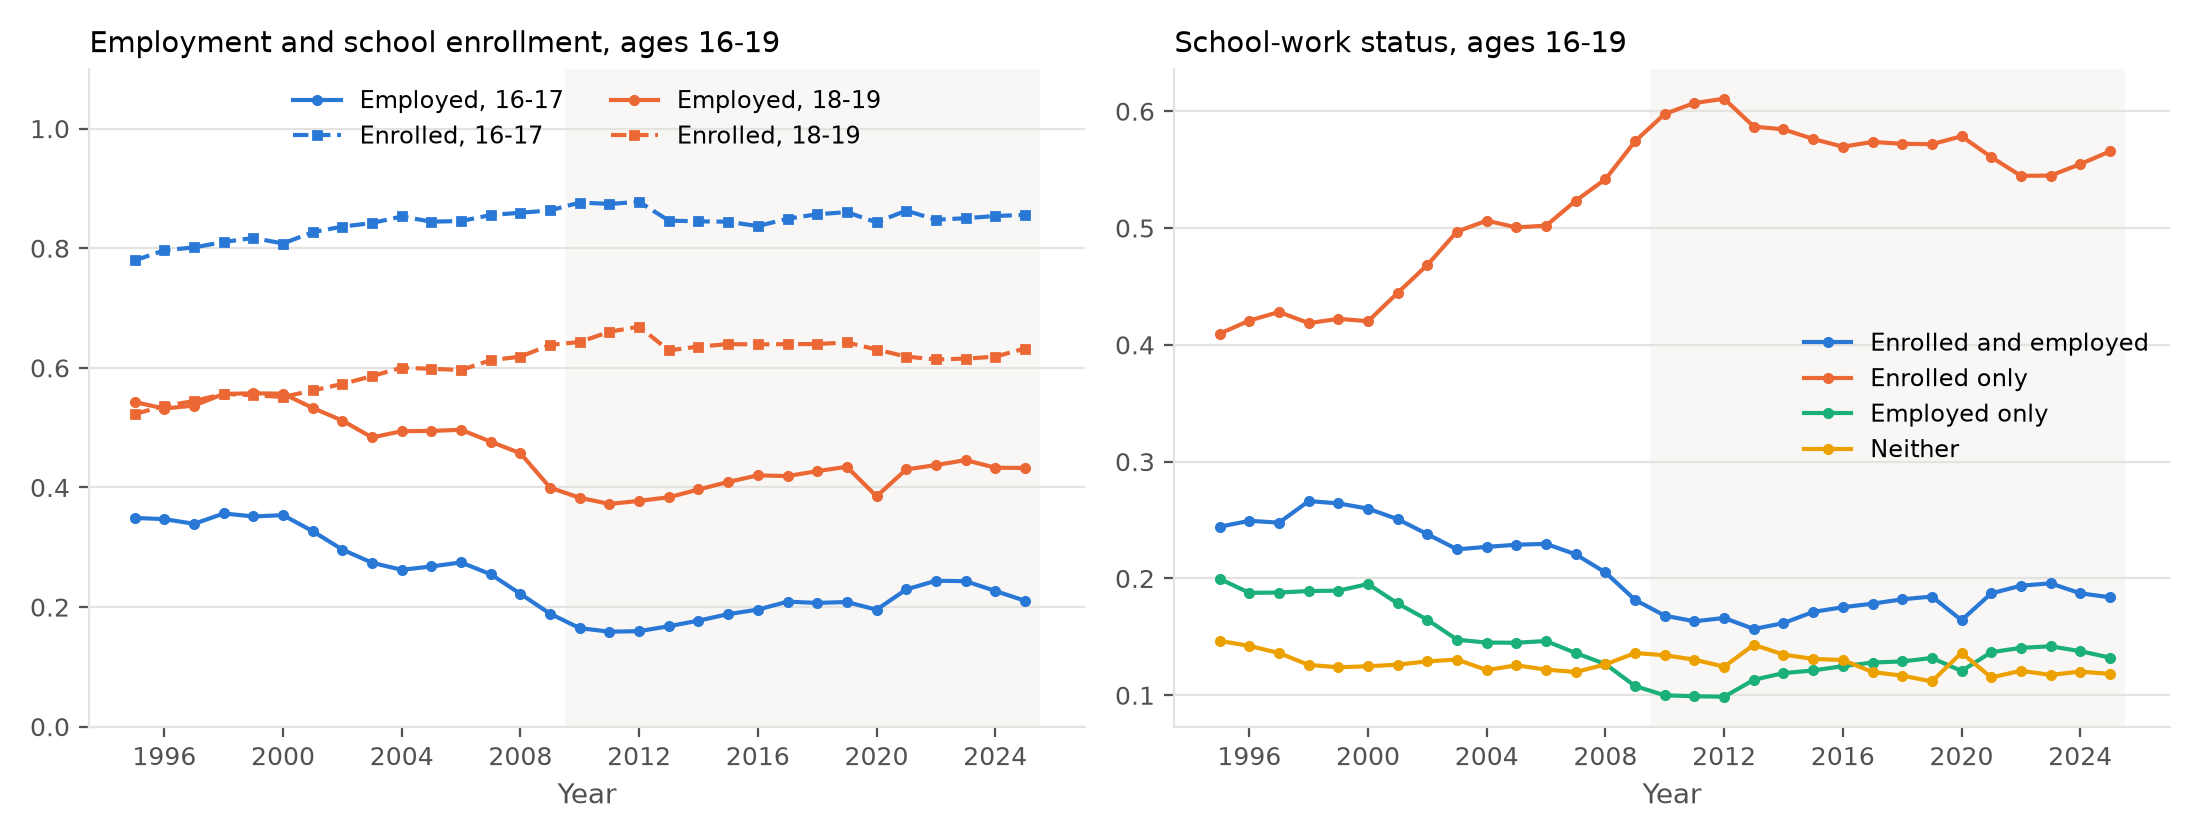
\includegraphics[width=\textwidth]{figures/fig1_trends.png}

\caption{Figure 1: Employment, school enrollment and school--work status of 16--19 year olds, 2007--2025}



\noindent\small Notes: Annual weighted means from the CPS basic monthly files, all months.
\end{figure}

\begin{figure}
\centering

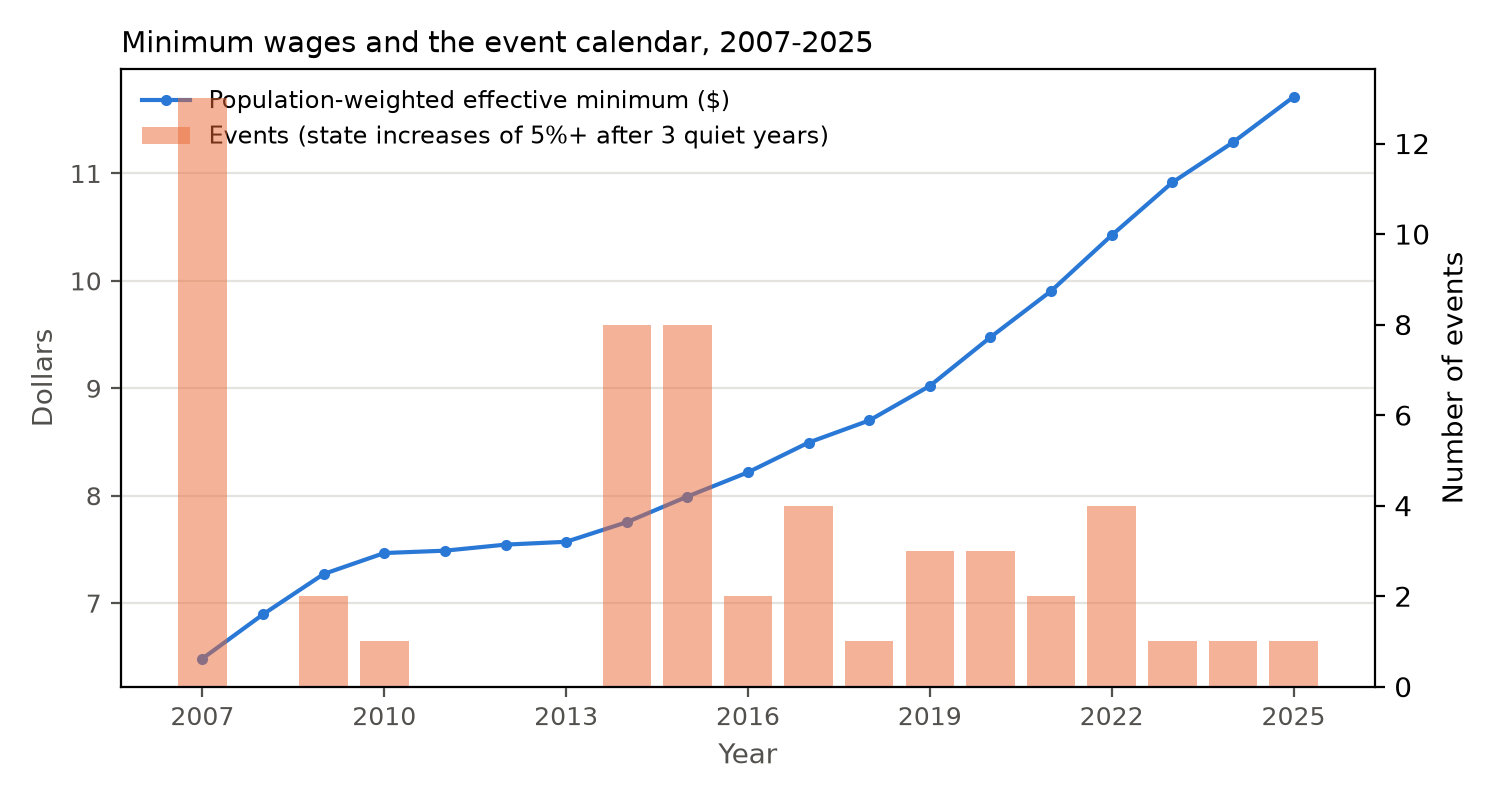
\includegraphics[width=0.85\textwidth]{figures/fig2_minwage.png}

\caption{Figure 2: The effective minimum wage and the calendar of state events, 2007--2025}



\noindent\small Notes: Line: mean of the larger of the state and federal minimum, weighted by the state's teen population. Bars: number of state-driven increases of at least 5 percent after 36 months without one.
\end{figure}

\begin{table}
\centering
\caption{Table 1: Means in the year before the event, 39 state events from 2010: event states and clean controls}

\small
\begin{tabular}{lrrrr}
\toprule
 & \multicolumn{2}{c}{Ages 16--17} & \multicolumn{2}{c}{Ages 18--19} \\

 & Event states & Controls & Event states & Controls \\
\midrule
Enrolled in school & 0.854 & 0.843 & 0.644 & 0.609 \\
Employed & 0.185 & 0.211 & 0.393 & 0.431 \\
In labor force & 0.227 & 0.255 & 0.471 & 0.507 \\
Enrolled and employed & 0.135 & 0.157 & 0.196 & 0.209 \\
Enrolled only & 0.719 & 0.686 & 0.448 & 0.400 \\
Employed only & 0.050 & 0.055 & 0.197 & 0.222 \\
Neither & 0.096 & 0.102 & 0.159 & 0.168 \\
Usual weekly hours (0 if not working) & 3.18 & 3.67 & 9.86 & 11.32 \\
Hourly wage, hourly paid (\$) & 9.61 & 9.20 & 10.69 & 10.12 \\
Female & 0.487 & 0.497 & 0.498 & 0.494 \\
Black & 0.126 & 0.174 & 0.130 & 0.177 \\
Hispanic & 0.242 & 0.186 & 0.249 & 0.193 \\
Person-months & 29,115 & 763,850 & 26,859 & 665,432 \\
\bottomrule
\end{tabular}



\noindent\small Notes: Weighted means over the twelve months before each event, pooled across events. Hourly wage among hourly-paid workers in the outgoing rotation groups, earnings-weighted.

\end{table}

\section{4 Empirical Strategy}

\subsection{4.1 Units}

The minimum wage a teenager faces is set by the state and, in a growing number of places, by the city or county. Sixty cities and counties set minimums above their state's between 2004 and 2025, from San Francisco and Santa Fe in 2004 to Seattle, Chicago, Los Angeles and the Minneapolis--St.\ Paul cities in the following decade. The geographic units of the analysis are therefore the jurisdictions whose wage floor a teen faces: each identified county with a local minimum is a unit with its own effective minimum wage series, the local rate applied to the whole county, and the remainder of each state, its teens outside those counties, is a unit at the state rate. There are 107 units, 56 of them counties in 13 states, and the effective minimum of a unit in a month is the larger of its own rate and the federal minimum. A Seattle teen is at Seattle's minimum, a teen elsewhere in Washington at the state's, and when Seattle raises its minimum King County has an event of its own.

\subsection{4.2 Events and clean controls}

The minimum wage is a continuous policy that most jurisdictions now change every January by legislation or indexation, so it cannot be used as a once-and-for-all treatment. Following Cengiz et al. (2019), I define events. An event occurs in unit $u$ and month $t$ if the unit's effective minimum rises by at least 5 percent because of state or local law and there has been no such rise in the unit in the preceding 36 months. Later increases in the following 48 months, which in the modern schedules are the subsequent steps of the same law, are part of the same event, so a multi-year schedule is one event and its dose is the cumulative rise over the window. Increases caused by a change in the federal minimum are not events. This yields 101 unit events from January 2010, of which 73 have CPS teens in the unit (Appendix Table 23): 39 in state remainders, 18 in counties where state and local rates rose together, and 16 driven by a local rise alone. The events raise the minimum by 5 to 86 percent over the window, 38 percent on average, in 62 cases through two or more steps.

The controls for an event are the units in other states that had no qualifying increase in the window from 36 months before the event to 47 months after it. For the events from 2010 on, the federal minimum did not change, so these units had no change in their minimum at all; each event has a median of 28 such controls. The windows of the four events of 2010--2013 begin before the federal increase of July 2009, which raised the minimum in treated and control units alike and is absorbed by the comparison with the year before the event. No events before 2010 are used, and no observations before January 2007 enter any estimate.

\subsection{4.3 Estimator}

For event $e$ in unit $u_e$ at month $t_e$, define relative year $k = \lfloor (t - t_e)/12 \rfloor$, so that $k = -1$ is the twelve months before the increase, $k = 0$ the twelve months starting with it, and $k = 3$ the fourth year after. Let $\bar{y}^T_{e,k}$ be the weighted mean of an outcome among teens in the treated unit in relative year $k$, and $\bar{y}^C_{e,k}$ the same among teens in the pooled control units. The event-specific effect in relative year $k$ is
\begin{equation}
\hat\tau_{e,k} = \left( \bar{y}^T_{e,k} - \bar{y}^T_{e,-1} \right) - \left( \bar{y}^C_{e,k} - \bar{y}^C_{e,-1} \right), \qquad k \in \{-3,-2,0,1,2,3\},

\end{equation}
which is the group-time average treatment effect of Callaway and Sant'Anna (2021) for a single cohort with the base period fixed at the year before treatment, and the coefficient a stacked regression with event-by-unit and event-by-year fixed effects recovers. The aggregate effect at relative year $k$ is $\hat\tau_k = \sum_e \omega_e \hat\tau_{e,k}$, with $\omega_e$ proportional to the treated unit's teen population in the base year, and the post-event average is the mean of $\hat\tau_0$ to $\hat\tau_3$. Because each event's controls are chosen to be untreated throughout its window, the design uses none of the comparisons between earlier- and later-treated units that bias two-way fixed effects estimates (Goodman-Bacon, 2021; de Chaisemartin and D'Haultf{\oe}uille, 2020; Sun and Abraham, 2021; Baker et al., 2022). The state remainders carry most of the population weight; the county units add 34 events, including the largest local increases.

Inference is by block bootstrap over states: in each of 99 draws the 51 states are resampled with replacement, every unit moves with its state, the event effects are recomputed with treated units entering as many times as their state is drawn and controls weighted by their multiplicity, and the standard error is the standard deviation of the aggregate across draws. This treats the state as the unit of both policy and sampling and accounts for the repeated observation of the same teens across months. The Stata implementation in the replication files runs the stacked regression with the wild cluster bootstrap and the estimator of de Chaisemartin and D'Haultf{\oe}uille (2024) on the log minimum wage as a continuous treatment.

Identification requires that, absent the increase, teens in the treated unit would have followed the same path as teens in the control units over the seven-year window. The three pre-event coefficients test the assumption directly. Because the events are laws passed by legislatures, councils and ballot measures, and treated jurisdictions are on average richer and more urban than federal-floor states, the assumption is about trends rather than levels, and Section 6 shows the results with control sets that vary from all clean units to federal-floor states only, with equal weights, without the pandemic years, in school months only, and with states rather than counties as the units.

\subsection{4.4 Regression counterpart}

Each event-study figure is preceded by a table with the stacked regression form of the event design (Cengiz et al., 2019):
\begin{equation}
y_{i,e,t} = \delta\, \mathrm{Post}_{e,t} \times \mathrm{Treated}_{e,u(i)} + X_i'\gamma + \alpha_{e,u(i)} + \lambda_{e,t} + \varepsilon_{i,e,t},

\end{equation}
estimated on every teen observation in the 84 months from $-36$ to $+47$ around each of the 73 events, the treated unit and its clean controls, with event-by-unit and event-by-month fixed effects, dummies for single year of age, sex, race and Hispanic origin (non-Hispanic white, Black, Hispanic, other) and the CPS family income category, survey weights, and standard errors clustered by state. The stacked file has 6.8 million observations at 16--17, 6.3 million at 18--19 and 13.1 million pooled, built from 620,000, 554,000 and 1.17 million teen-months, each control unit's teens entering the blocks of every event for which the unit is a clean control. $\delta$ is a single post-event average on the same footing as the mean of $\hat\tau_0$ to $\hat\tau_3$; it differs from that mean in taking all 36 pre-event months rather than the twelve of year $-1$ as the base, in weighting observations rather than events, and in the individual controls, so the two need not coincide exactly. Without the controls the regression is numerically the regression on unit-month cell means, and the controls move no school--work coefficient by more than a quarter of a point and no wage or earnings coefficient by more than about a point. Appendix C reports the two-way fixed effects regression of the outcome on the log minimum wage, the specification of Neumark and Shupe (2019) and Smith (2021), and shows where it agrees with the event design and where it does not.

\section{5 Results}

\subsection{5.1 School and work}

Appendix Table 15 reports the post-event average effect of the increases on the four school--work shares for ages 16--17, 18--19 and 16--19 pooled, with the average of the pre-event coefficients beside each estimate; the last two rows give enrollment and employment, which are sums of the shares. Nothing moves. The share enrolled and employed changes by $-0.3$ points (s.e.\ 0.5) at 16--17 and $+0.7$ (0.6) at 18--19; enrolled only by $-0.0$ (0.6) and $-0.5$ (0.6); employed only by $+0.2$ (0.3) and $+0.3$ (0.7); neither enrolled nor employed by $+0.1$ (0.4) and $-0.5$ (0.5). Enrollment changes by $-0.3$ (0.4) and $+0.1$ (0.9), so the 95 percent intervals exclude a fall larger than 1.1 points at the younger ages and 1.6 at the older; employment by $-0.1$ (0.5) and $+1.0$ (0.7). The pre-event averages are of the same order as the post-event ones and of no consistent sign.


Table 2 gives the stacked difference-in-differences coefficients of Section 4.4, one post-event average per share and age. They reproduce the event-study averages of Appendix Table 15: $-0.1$ points (s.e.\ 0.4) for enrolled-and-employed at 16--17 and $+0.4$ (0.5) at 18--19, $-0.1$ (0.5) and $-0.7$ (0.6) for enrolled only, $+0.3$ (0.2) and $+0.5$ (0.6) for employed only, $-0.1$ (0.3) and $-0.3$ (0.4) for neither, and nothing beyond about one standard error from zero for any share or age. The two-way fixed effects regression of the earlier literature, reported in Appendix C, agrees with these estimates in school months and departs from them only when the summer months, in which the enrollment item records summer school, are included.

\begin{table}
\centering
\caption{Table 2: Stacked difference-in-differences estimates for teen school--work status, 73 events from 2010}

\small
\begin{tabular}{p{0.30\textwidth}p{0.227\textwidth}p{0.227\textwidth}p{0.227\textwidth}}
\toprule
 & Ages 16--17 & Ages 18--19 & Ages 16--19 \\
\midrule
Enrolled and employed & -0.001 & 0.004 & 0.002 \\
 & (0.004) & (0.005) & (0.003) \\
Enrolled only & -0.001 & -0.007 & -0.004 \\
 & (0.005) & (0.006) & (0.004) \\
Employed only & 0.003 & 0.005 & 0.004 \\
 & (0.002) & (0.006) & (0.003) \\
Neither enrolled nor employed & -0.001 & -0.003 & -0.002 \\
 & (0.003) & (0.004) & (0.002) \\
Enrolled & -0.002 & -0.002 & -0.002 \\
 & (0.003) & (0.007) & (0.004) \\
Employed & 0.002 & 0.009 & 0.006 \\
 & (0.005) & (0.006) & (0.004) \\
\bottomrule
\end{tabular}



\noindent\small Notes: Coefficient on post $\times$ treated in regression (6): teen observations stacked over the 73 events with their clean controls, 36 months before to 47 months after the increase, event-by-unit and event-by-month fixed effects, dummies for age, sex, race and Hispanic origin and family income category, survey weights. Standard errors clustered by state in parentheses. \textsuperscript{*}, \textsuperscript{**}, \textsuperscript{***}: significant at 10, 5 and 1 percent.

\end{table}

Figure 3 plots the coefficients by relative year for each share and age bracket. Every post-event point sits inside an interval that includes zero, and the pre-event points look the same as the post-event ones. Enrolled-and-employed at 18--19 drifts up by about half a point and enrolled-only down by the same, which is the mirror image and within noise. The shift from enrolled-and-employed to enrolled-only that Neumark and Shupe (2019) attribute to the minimum wage would appear as a fall in the first panel and a rise in the second; if anything the movements are in the opposite direction.

\begin{figure}
\centering

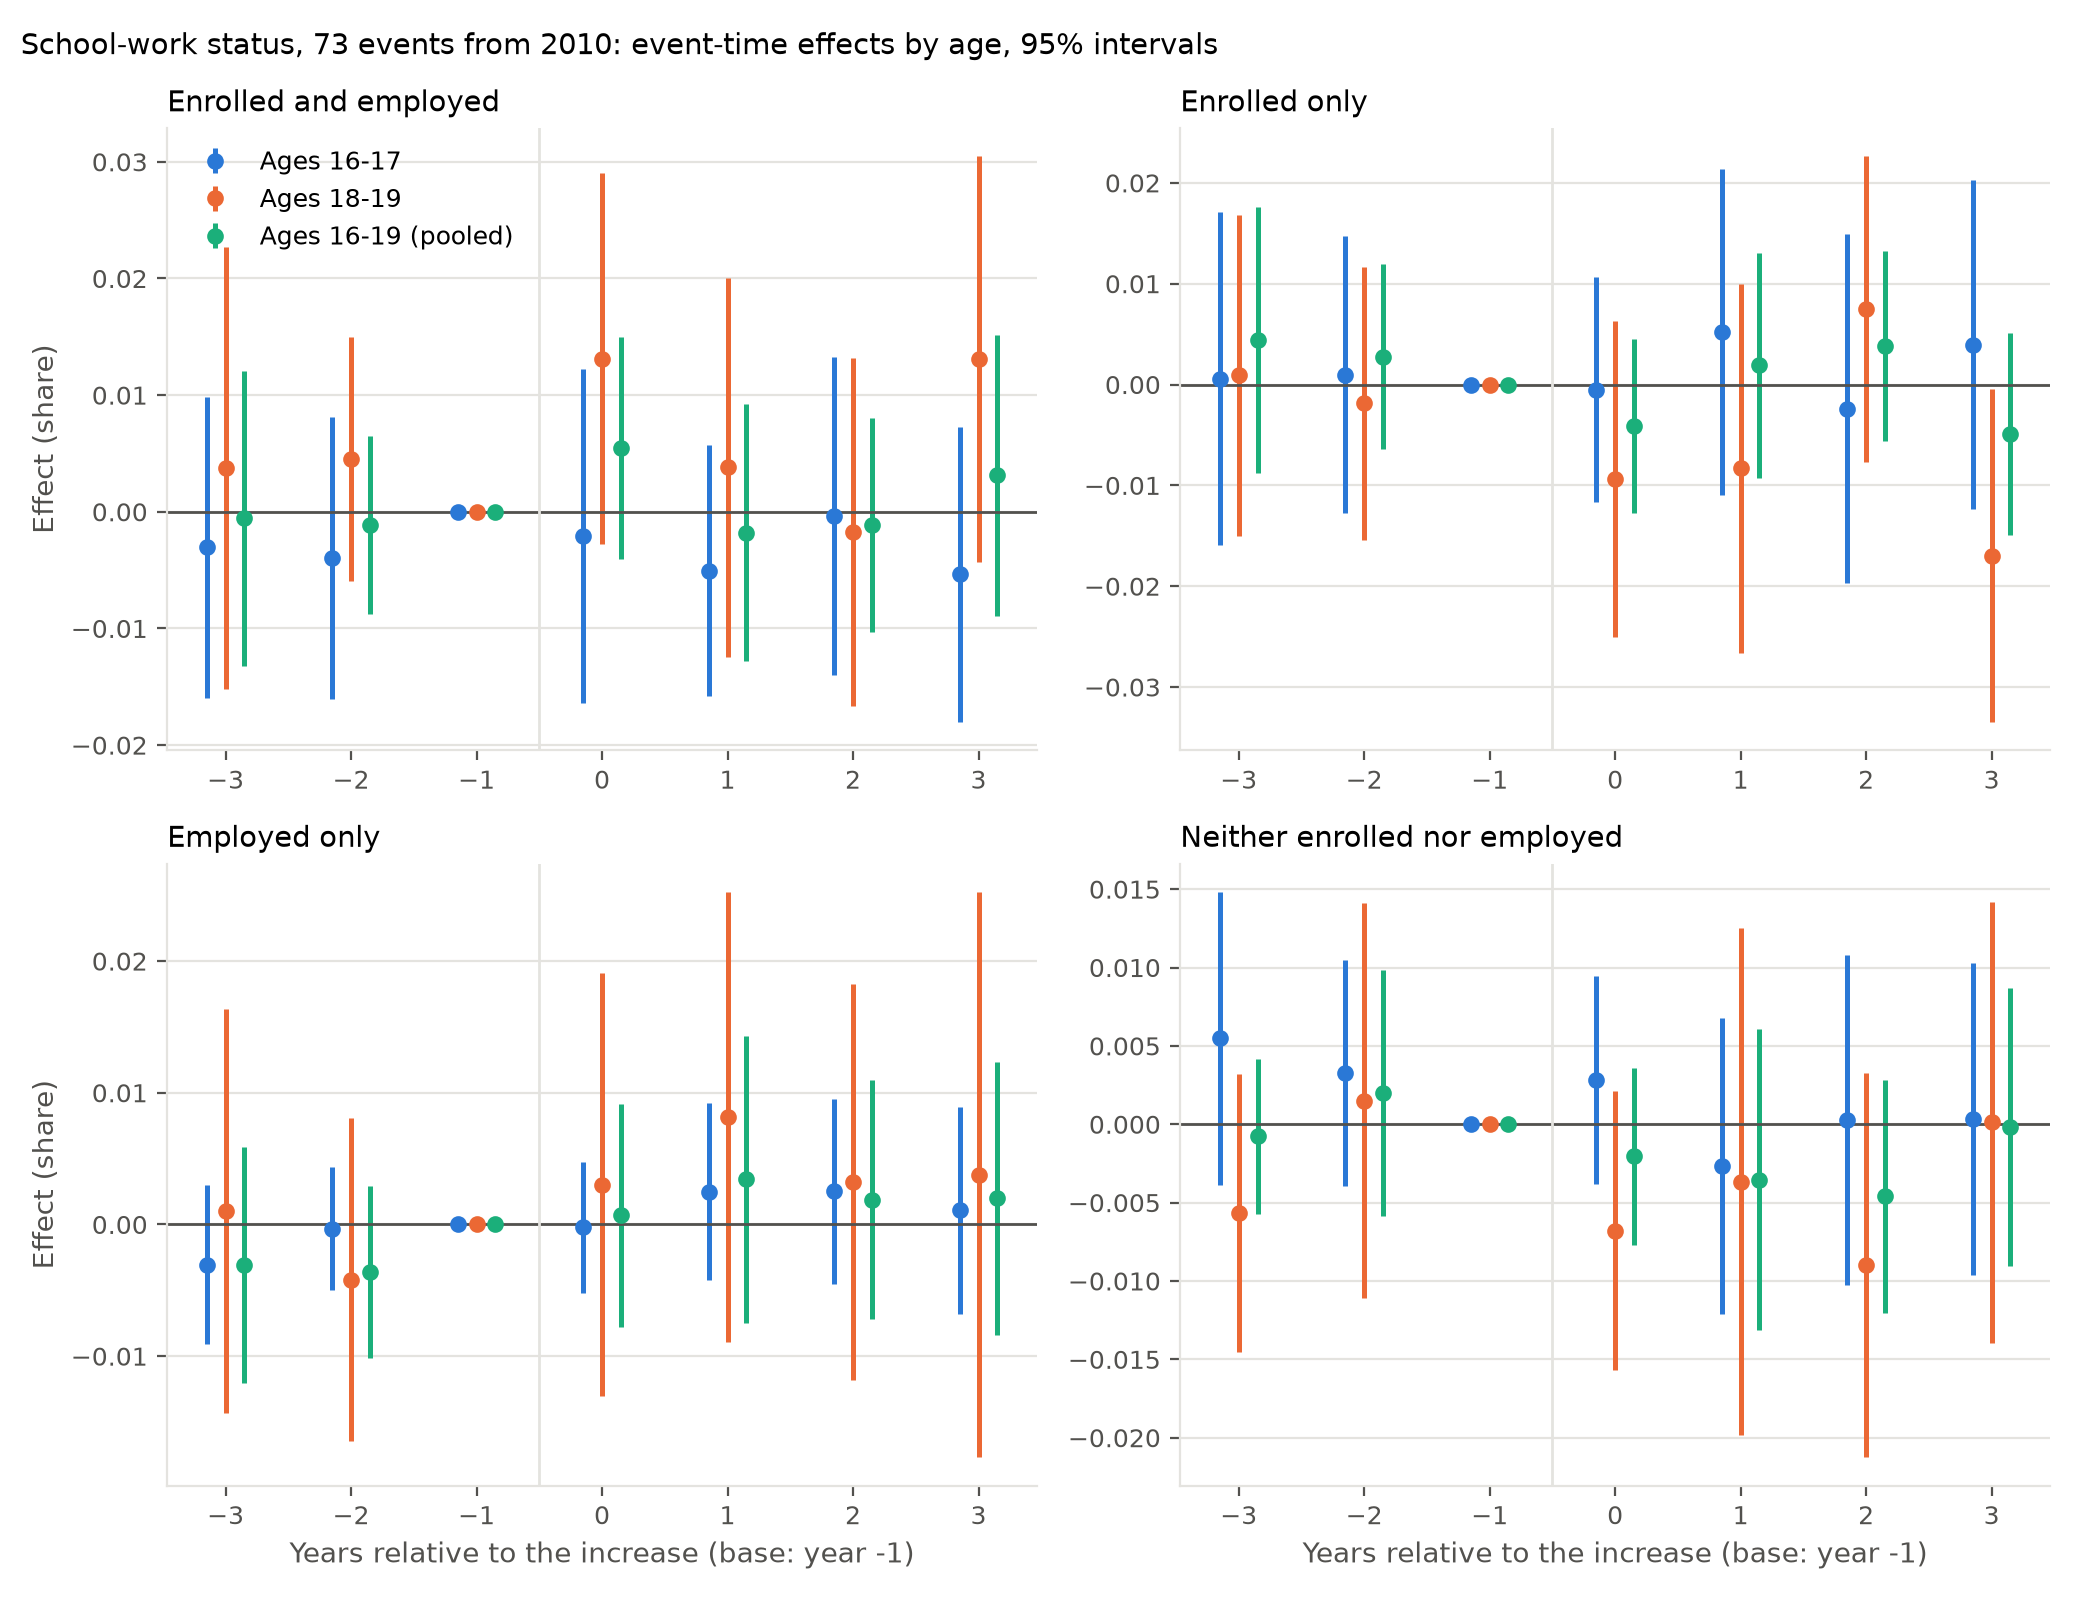
\includegraphics[width=\textwidth]{figures/figR1_groups.png}

\caption{Figure 3: Event-time effects on the four school--work shares, by age, 73 events from 2010}



\noindent\small Notes: Effects relative to the year before the increase, population-weighted across events; 95 percent intervals from the state block bootstrap.
\end{figure}

\subsection{5.2 School and work by socioeconomic standing}

The theory of Section 2 and the evidence of Ehrenberg and Marcus (1982) and Smith (2021) put the schooling response, if there is one, among teens from poorer families: the opportunity-cost channel binds hardest where the alternative to school is a minimum wage job, and the liquidity channel operates only where the family cannot pay for school. Smith (2021) finds that a 10 percent rise in the state minimum lowers dropout by 0.5 to 1.0 points among teens whose parents lack a diploma and does nothing for the rest. The CPS basic monthly files identify the family's income category, so I split teens by family income below versus at or above \$50,000, close to the median for teen households over the period; Appendix D repeats the analysis with a split at the weighted median income category among teens in the same survey year, which removes the drift of a nominal threshold (45 percent of teens were below \$50,000 in 2007, 28 percent in 2024). Smith (2021) reports his own estimates with income-percentile splits and finds the effect concentrated in the bottom of the distribution and shrinking as the threshold rises toward the median, so a median split is a test of the same claim at a coarser cut.

Appendix Tables 16 and 17 give the post-event averages for the four shares by family income and age, and Figure 4 plots the event-time coefficients for the pooled ages. No share differs by income. For low-income teens, enrolled-and-employed changes by $+0.4$ points (s.e.\ 0.8) at 16--17 and $+0.6$ (0.8) at 18--19, enrolled-only by $-0.5$ (1.0) and $-0.2$ (0.9), employed-only by $-0.2$ (0.4) and $+0.6$ (1.1), neither by $+0.3$ (0.5) and $-1.0$ (0.7); for high-income teens the corresponding figures are $-0.6$ (0.5) and $+0.9$ (0.9), $+0.2$ (0.6) and $-0.6$ (0.8), $+0.5$ (0.3) and $+0.3$ (0.9), $-0.1$ (0.4) and $-0.5$ (0.6). Enrollment among low-income teens changes by $-0.1$ (0.6) at 16--17 and $+0.4$ (1.2) at 18--19. The low-minus-high differences are within one standard error of zero for every share and age, and the within-year median split in the appendix gives the same picture. The prediction of the liquidity channel, a rise in enrollment among poorer teens, does not appear: the low-income enrollment interval at 16--17 excludes a rise larger than 1.1 points.


The stacked coefficients in Table 3 repeat the pattern within each income group. The only coefficient beyond two standard errors is employed-only among high-income 16--17 year olds, $+0.5$ points (s.e.\ 0.2), a rise; the neither share changes by $-0.3$ (0.5) for low-income and $-0.1$ (0.3) for high-income 16--17 year olds.

\begin{table}
\centering
\caption{Table 3: Stacked difference-in-differences estimates for school--work status by family income}

\small
\begin{tabular}{p{0.30\textwidth}p{0.113\textwidth}p{0.113\textwidth}p{0.113\textwidth}p{0.113\textwidth}p{0.113\textwidth}p{0.113\textwidth}}
\toprule
 & \multicolumn{2}{c}{Ages 16--17} & \multicolumn{2}{c}{Ages 18--19} & \multicolumn{2}{c}{Ages 16--19} \\

 & Low & High & Low & High & Low & High \\
\midrule
Enrolled and employed & -0.000 & -0.000 & -0.001 & 0.008 & -0.000 & 0.004 \\
 & (0.006) & (0.004) & (0.005) & (0.007) & (0.003) & (0.005) \\
Enrolled only & 0.003 & -0.003 & 0.003 & -0.009 & 0.003 & -0.007 \\
 & (0.007) & (0.004) & (0.009) & (0.006) & (0.007) & (0.005) \\
Employed only & -0.000 & 0.005\textsuperscript{**} & 0.002 & 0.005 & 0.001 & 0.005 \\
 & (0.003) & (0.002) & (0.008) & (0.007) & (0.005) & (0.004) \\
Neither enrolled nor employed & -0.003 & -0.001 & -0.005 & -0.003 & -0.004 & -0.002 \\
 & (0.005) & (0.003) & (0.006) & (0.004) & (0.004) & (0.003) \\
\bottomrule
\end{tabular}



\noindent\small Notes: Low: family income below \$50,000; High: \$50,000 or more. Specification as in Table 2; standard errors clustered by state in parentheses.

\end{table}

\begin{figure}
\centering

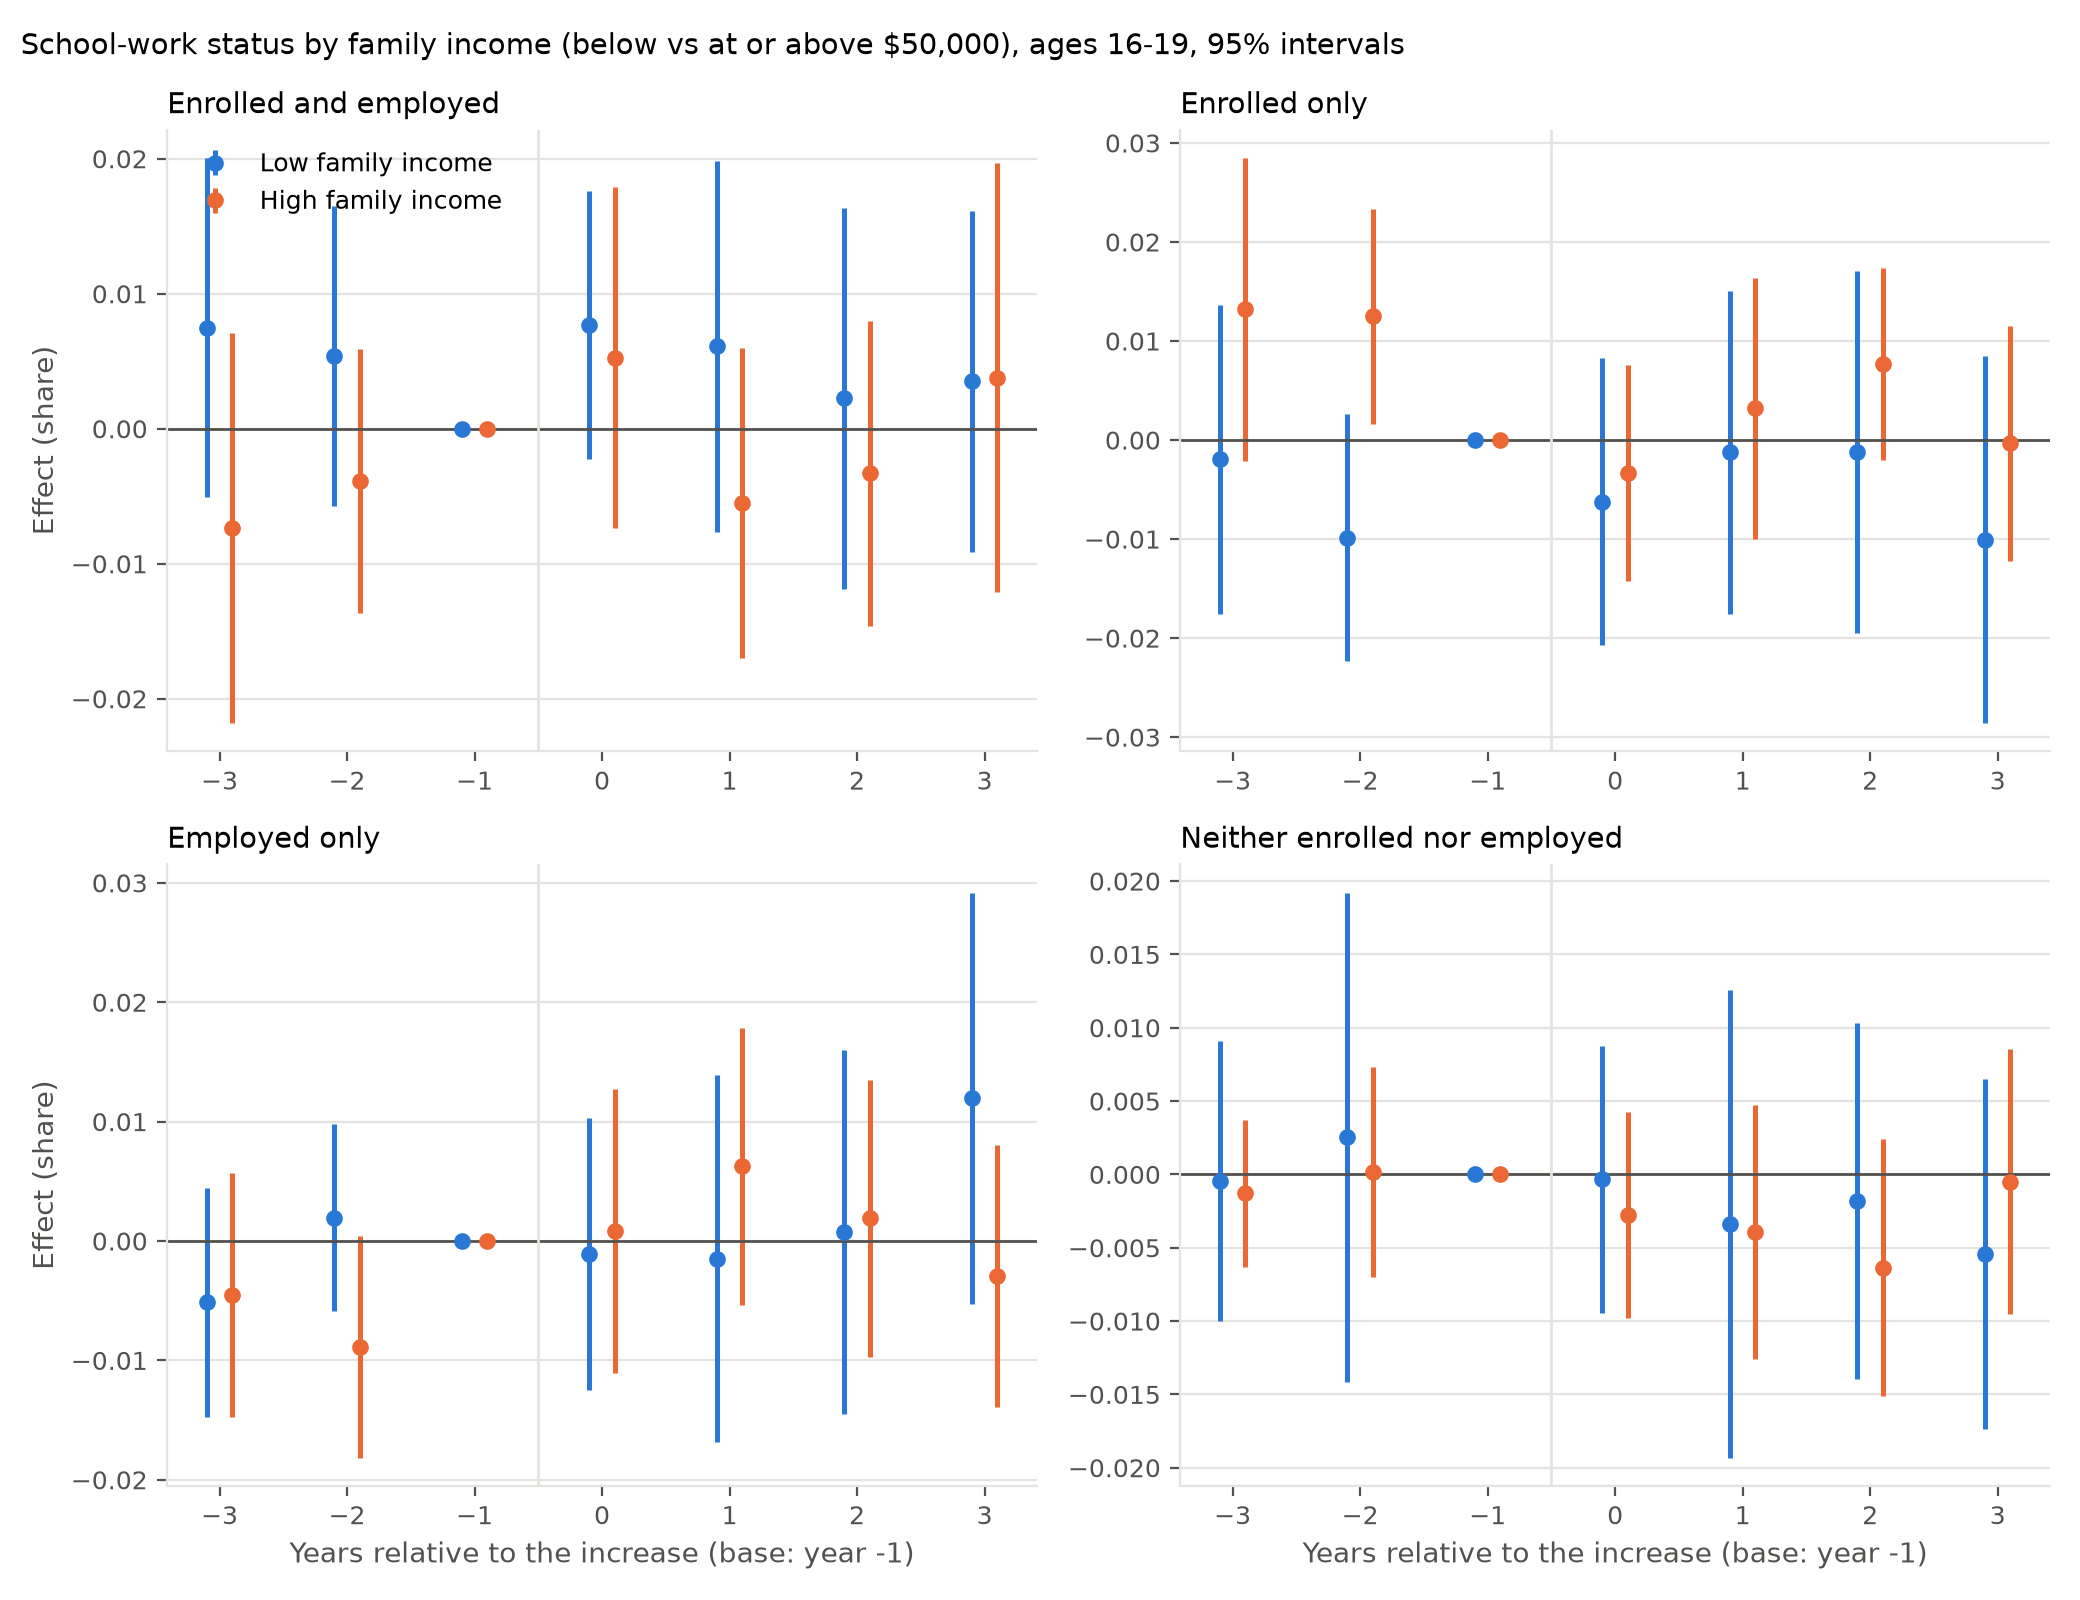
\includegraphics[width=\textwidth]{figures/figR2_groups_ses.png}

\caption{Figure 4: Event-time effects on the four school--work shares by family income, ages 16--19}

\end{figure}

\subsection{5.3 School and work by sex}

Girls and boys differ on both margins that the theory of Section 2 turns on. Over 2010--2026, 77 percent of 16--19 year old girls are enrolled and 31 percent employed, against 74 and 29 percent of boys, and hourly-paid girls earn \$10.84 an hour against \$11.71 for boys, so a rise in the minimum binds on more of the jobs girls hold. If the opportunity-cost channel operates, it should show first among girls, whose wage moves more; if the liquidity channel operates, it should show among whichever group is closer to the enrollment margin, which at 18--19 is boys. Appendix Tables 19 and 20 give the post-event averages for the four shares by sex and age, Table 4 the stacked coefficients, and Figure 5 the event-time coefficients for the pooled ages.

The one cell in the paper where the shares move is girls aged 16--17. Their share enrolled and employed falls by 1.3 points (s.e.\ 0.5) and their employment by the same 1.3 (0.5), with pre-event averages of 0.0, and their share enrolled only rises by 1.2 (0.7), so enrollment is unchanged ($-0.1$, s.e.\ 0.5) and the movement is out of work and into school only, the shift that Neumark and Shupe (2019) describe. Boys of the same age move the other way, $+0.8$ (1.0) on enrolled-and-employed and $+1.2$ (0.9) on employment, so the girl--boy difference on employment is $-2.5$ points with a standard error of about 1.0. At 18--19 girls' four shares change by $+0.8$ (1.0), $+0.5$ (0.9), $-0.2$ (0.9) and $-1.1$ (0.8), with pre-event averages of the same size and sign ($+1.4$, $+1.8$, $-1.8$, $-1.4$), which is drift rather than response, and boys' by $+0.5$ (0.7), $-1.6$ (0.9), $+0.9$ (0.9) and $+0.1$ (0.6). Pooling the ages, girls' employment changes by $-0.6$ (0.6) and boys' by $+1.3$ (0.6). The girls' estimate at 16--17 is one of 36 cells in the sex split and the only one beyond two standard errors; the wage first stage for girls at that age, 5.4 percent (1.9), is no larger than boys' 4.7 (1.7); and in Figure 5 the pooled enrolled-only series for girls sits about a point above the boys' series after the increases but also in the two years before them, so the divergence between the sexes is not timed to the events. I read the 16--17 estimate as the upper bound of what the design can find: a fall of about one point in the employment of the youngest girls, balanced by more schooling only, and no change in their enrollment. The stacked coefficients (Table 4) say the same. At 16--17, girls' enrolled-and-employed changes by $-1.2$ points (s.e.\ 0.6) and enrolled-only by $+1.0$ (0.7); boys' by $+1.0$ (0.6) and $-1.2$ (0.6). At 18--19 girls' four shares change by $-0.2$ (0.6), $-0.4$ (0.8), $+0.7$ (0.7) and $-0.1$ (0.5), and boys' by $+1.0$ (0.6), $-0.9$ (0.7), $+0.3$ (0.7) and $-0.4$ (0.5). Pooling the ages, boys shift about a point from enrolled-only to enrolled-and-employed ($+1.0$, s.e.\ 0.5, and $-1.1$, 0.5) and girls about half a point the other way ($-0.7$, 0.4, and $+0.3$, 0.7), which is why the two sexes cancel in Table 2: the pooled estimates are nulls because the sexes offset, not because nothing happens to either. Enrollment does not change for either sex at any age.

\begin{table}
\centering
\caption{Table 4: Stacked difference-in-differences estimates for school--work status by sex}

\small
\begin{tabular}{p{0.30\textwidth}p{0.113\textwidth}p{0.113\textwidth}p{0.113\textwidth}p{0.113\textwidth}p{0.113\textwidth}p{0.113\textwidth}}
\toprule
 & \multicolumn{2}{c}{Ages 16--17} & \multicolumn{2}{c}{Ages 18--19} & \multicolumn{2}{c}{Ages 16--19} \\

 & Girls & Boys & Girls & Boys & Girls & Boys \\
\midrule
Enrolled and employed & -0.012\textsuperscript{**} & 0.010\textsuperscript{*} & -0.002 & 0.010 & -0.007\textsuperscript{*} & 0.010\textsuperscript{**} \\
 & (0.006) & (0.006) & (0.006) & (0.006) & (0.004) & (0.005) \\
Enrolled only & 0.010 & -0.012\textsuperscript{**} & -0.004 & -0.009 & 0.003 & -0.011\textsuperscript{**} \\
 & (0.007) & (0.006) & (0.008) & (0.007) & (0.007) & (0.005) \\
Employed only & 0.000 & 0.006\textsuperscript{**} & 0.007 & 0.003 & 0.004 & 0.005 \\
 & (0.003) & (0.003) & (0.007) & (0.007) & (0.004) & (0.004) \\
Neither enrolled nor employed & 0.002 & -0.004 & -0.001 & -0.004 & 0.000 & -0.004 \\
 & (0.004) & (0.003) & (0.005) & (0.005) & (0.003) & (0.003) \\
\bottomrule
\end{tabular}



\noindent\small Notes: Specification as in Table 2; standard errors clustered by state in parentheses.

\end{table}

\begin{figure}
\centering

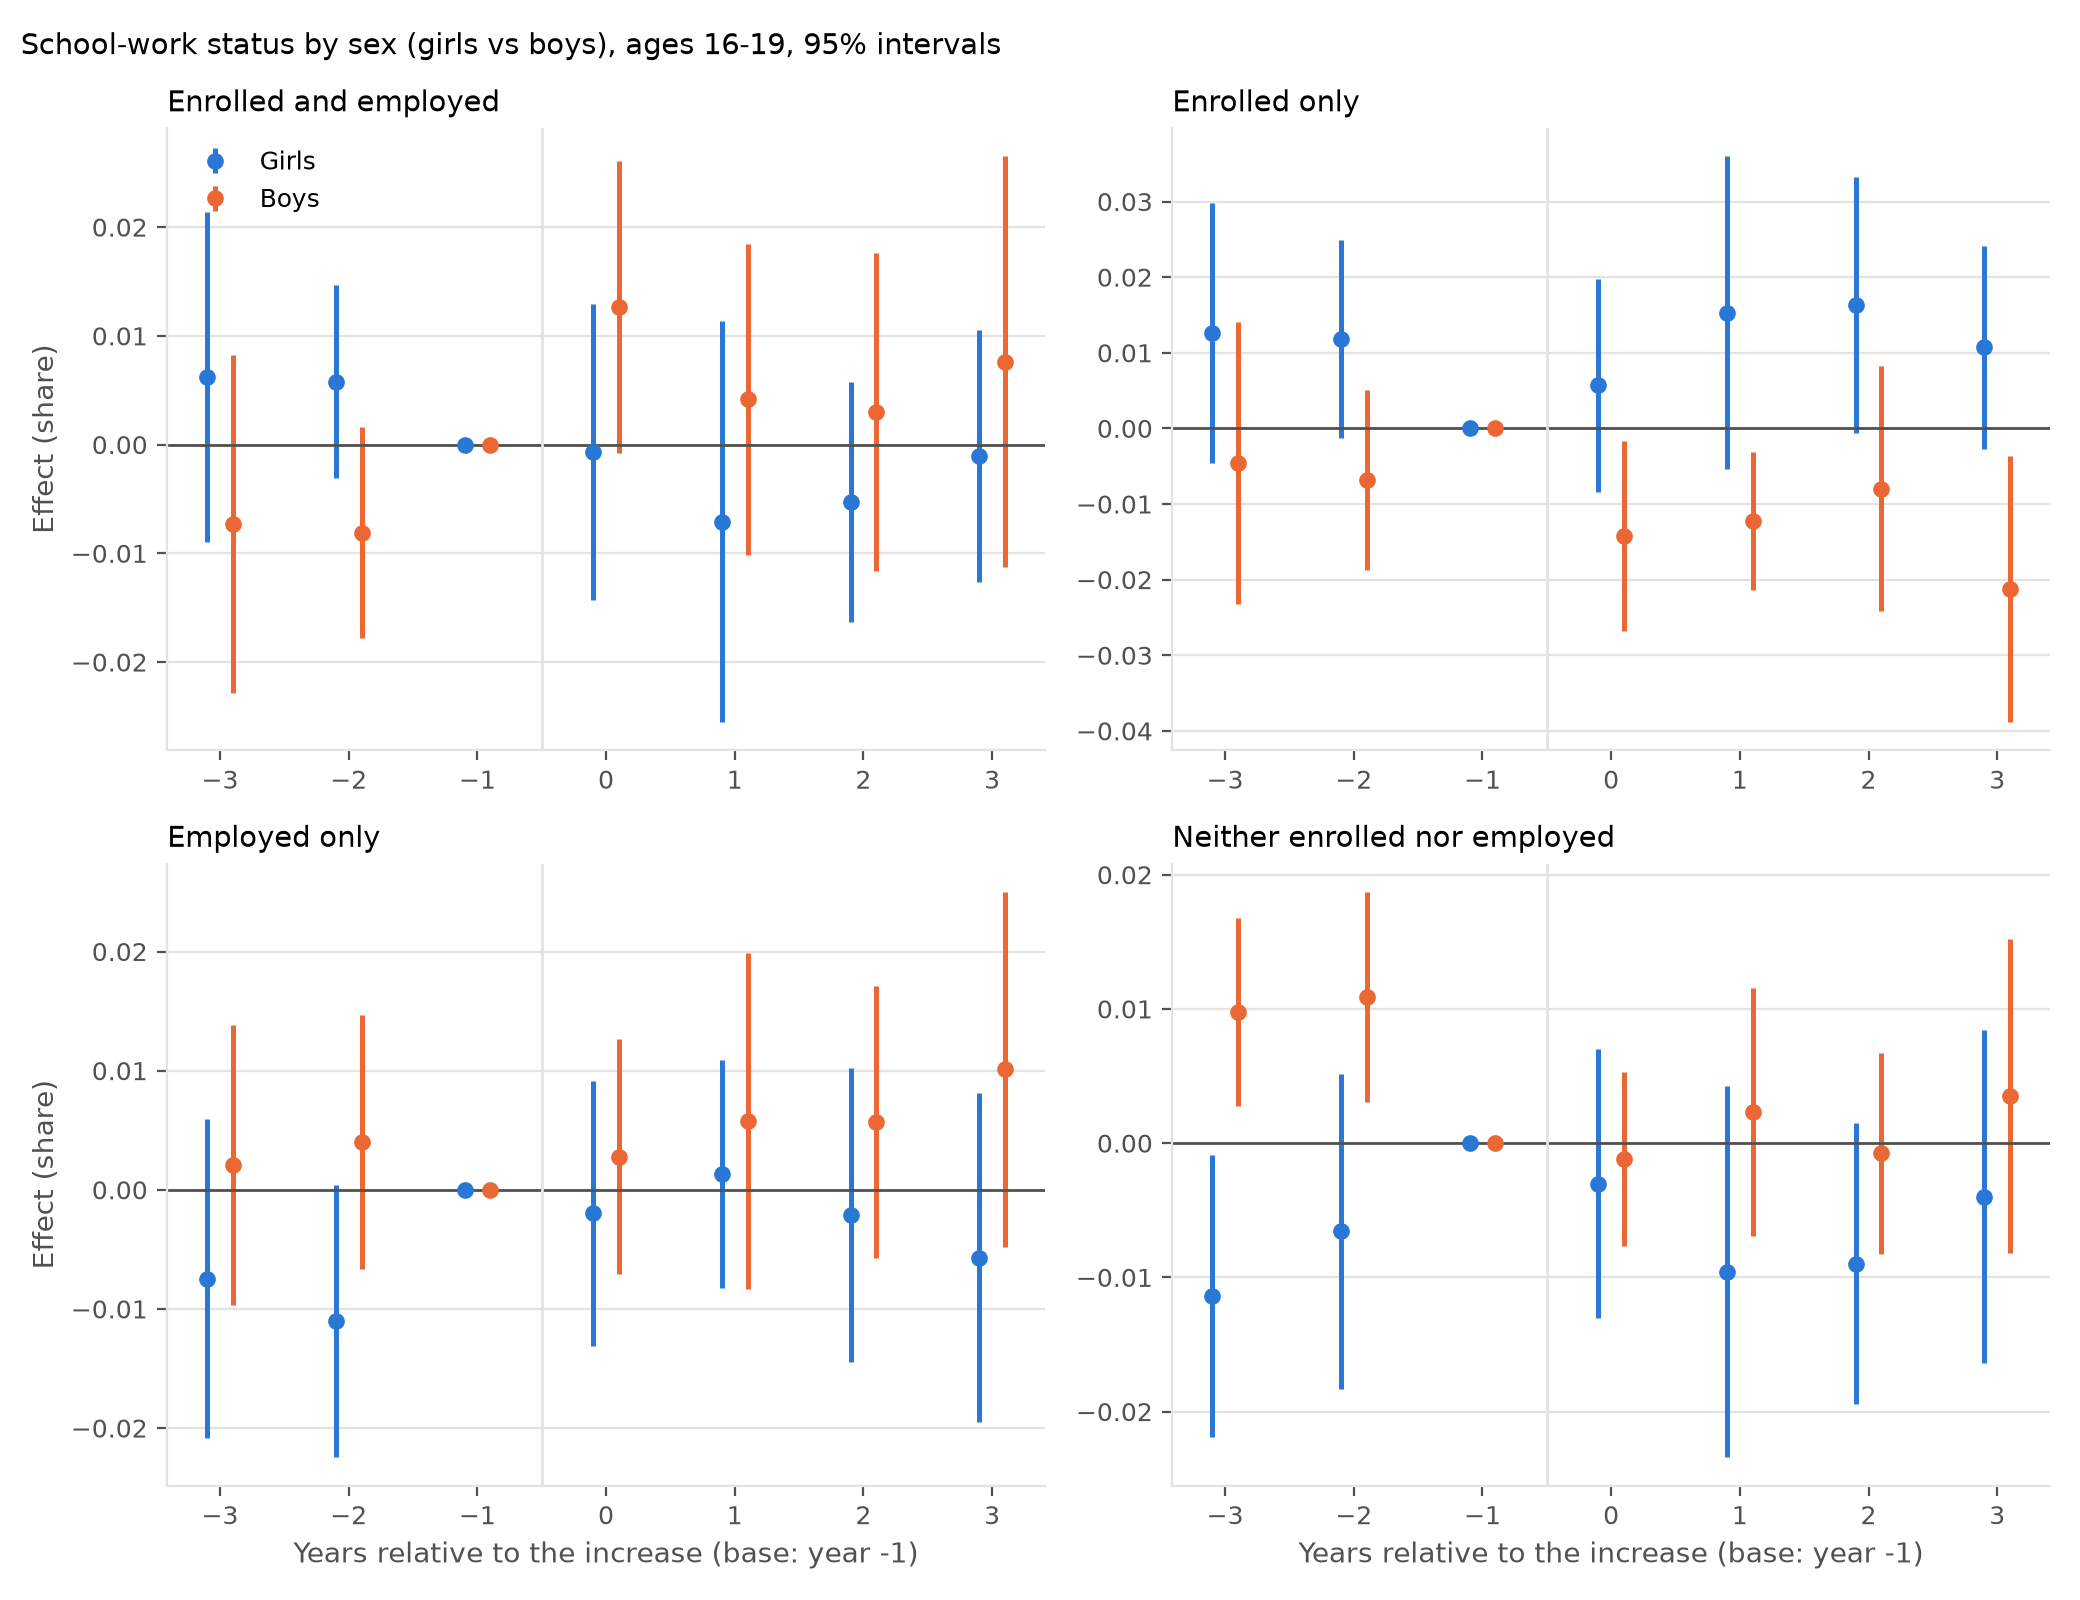
\includegraphics[width=\textwidth]{figures/figR2_groups_sex.png}

\caption{Figure 5: Event-time effects on the four school--work shares by sex, ages 16--19}

\end{figure}

\subsection{5.4 School and work by race}

Non-Hispanic white teens are 53 percent of 16--19 year olds over 2010--2026; the rest are Hispanic (half of the non-white group), Black (a third) and other. The two groups enroll at the same rate, 75 percent, but white teens are employed at 35 percent against 25 percent for non-white teens, and the share neither in school nor at work is 11 against 14 percent. Non-white teens are concentrated in the jurisdictions that raised their minimums, the large states of the West and Northeast and the big-city counties, so they carry more of the weight in the treated population than in the controls, and their families have lower incomes on average, so the liquidity channel, if it operates, should show among them. Appendix Tables 21 and 22 give the post-event averages by race and age, Table 5 the stacked coefficients, and Figure 6 the event-time coefficients for the pooled ages.

Nothing differs by race. For white teens the four shares change by $+0.3$ (s.e.\ 0.7), $-0.2$ (0.7), $+0.2$ (0.4) and $-0.3$ (0.5) at 16--17 and by $+0.0$ (1.0), $-0.9$ (0.8), $+0.6$ (1.0) and $+0.3$ (0.7) at 18--19; for non-white teens by $-1.2$ (0.7), $+0.7$ (1.2), $+0.1$ (0.4) and $+0.3$ (0.5), and by $+1.1$ (0.7), $+0.2$ (1.1), $-0.0$ (1.0) and $-1.2$ (0.8). Enrollment of non-white teens changes by $-0.4$ (0.7) at 16--17 and $+1.2$ (1.0) at 18--19, employment by $-1.1$ (0.9) and $+1.0$ (1.3), and the pooled estimates are within half a point of zero for every share. The non-white enrolled-and-employed estimate at 16--17 has the sign of the girls' estimate of Section 5.3, but it is under two standard errors, its pre-event average is $-0.3$, and the enrolled-only estimate beside it is $+0.7$ (1.2). The liquidity channel's prediction, a rise in enrollment among the group with lower family incomes, does not appear: the non-white enrollment interval at 16--17 excludes a rise larger than 1.0 point. The stacked coefficients (Table 5) agree. At 16--17 the white shares change by $+0.4$ (s.e.\ 0.5), $-0.7$ (0.7), $+0.3$ (0.3) and $-0.0$ (0.4), and the non-white shares by $-0.6$ (0.5), $+0.6$ (0.8), $+0.3$ (0.3) and $-0.3$ (0.4). The one coefficient beyond two standard errors is non-white enrolled-and-employed at 18--19, $+1.6$ (0.3), a rise, beside $-0.7$ (0.7) for white teens.

\begin{table}
\centering
\caption{Table 5: Stacked difference-in-differences estimates for school--work status by race}

\small
\begin{tabular}{p{0.30\textwidth}p{0.113\textwidth}p{0.113\textwidth}p{0.113\textwidth}p{0.113\textwidth}p{0.113\textwidth}p{0.113\textwidth}}
\toprule
 & \multicolumn{2}{c}{Ages 16--17} & \multicolumn{2}{c}{Ages 18--19} & \multicolumn{2}{c}{Ages 16--19} \\

 & White & Non-white & White & Non-white & White & Non-white \\
\midrule
Enrolled and employed & 0.004 & -0.006 & -0.007 & 0.016\textsuperscript{***} & -0.002 & 0.004 \\
 & (0.005) & (0.005) & (0.007) & (0.003) & (0.004) & (0.003) \\
Enrolled only & -0.007 & 0.006 & -0.004 & -0.005 & -0.006 & 0.001 \\
 & (0.007) & (0.008) & (0.008) & (0.009) & (0.006) & (0.007) \\
Employed only & 0.003 & 0.003 & 0.010 & -0.004 & 0.007\textsuperscript{*} & -0.000 \\
 & (0.003) & (0.003) & (0.007) & (0.008) & (0.004) & (0.004) \\
Neither enrolled nor employed & -0.000 & -0.003 & 0.001 & -0.007 & 0.001 & -0.005 \\
 & (0.004) & (0.004) & (0.005) & (0.005) & (0.003) & (0.004) \\
\bottomrule
\end{tabular}



\noindent\small Notes: White: non-Hispanic white; Non-white: Black, Hispanic and other. Specification as in Table 2; standard errors clustered by state in parentheses.

\end{table}

\begin{figure}
\centering

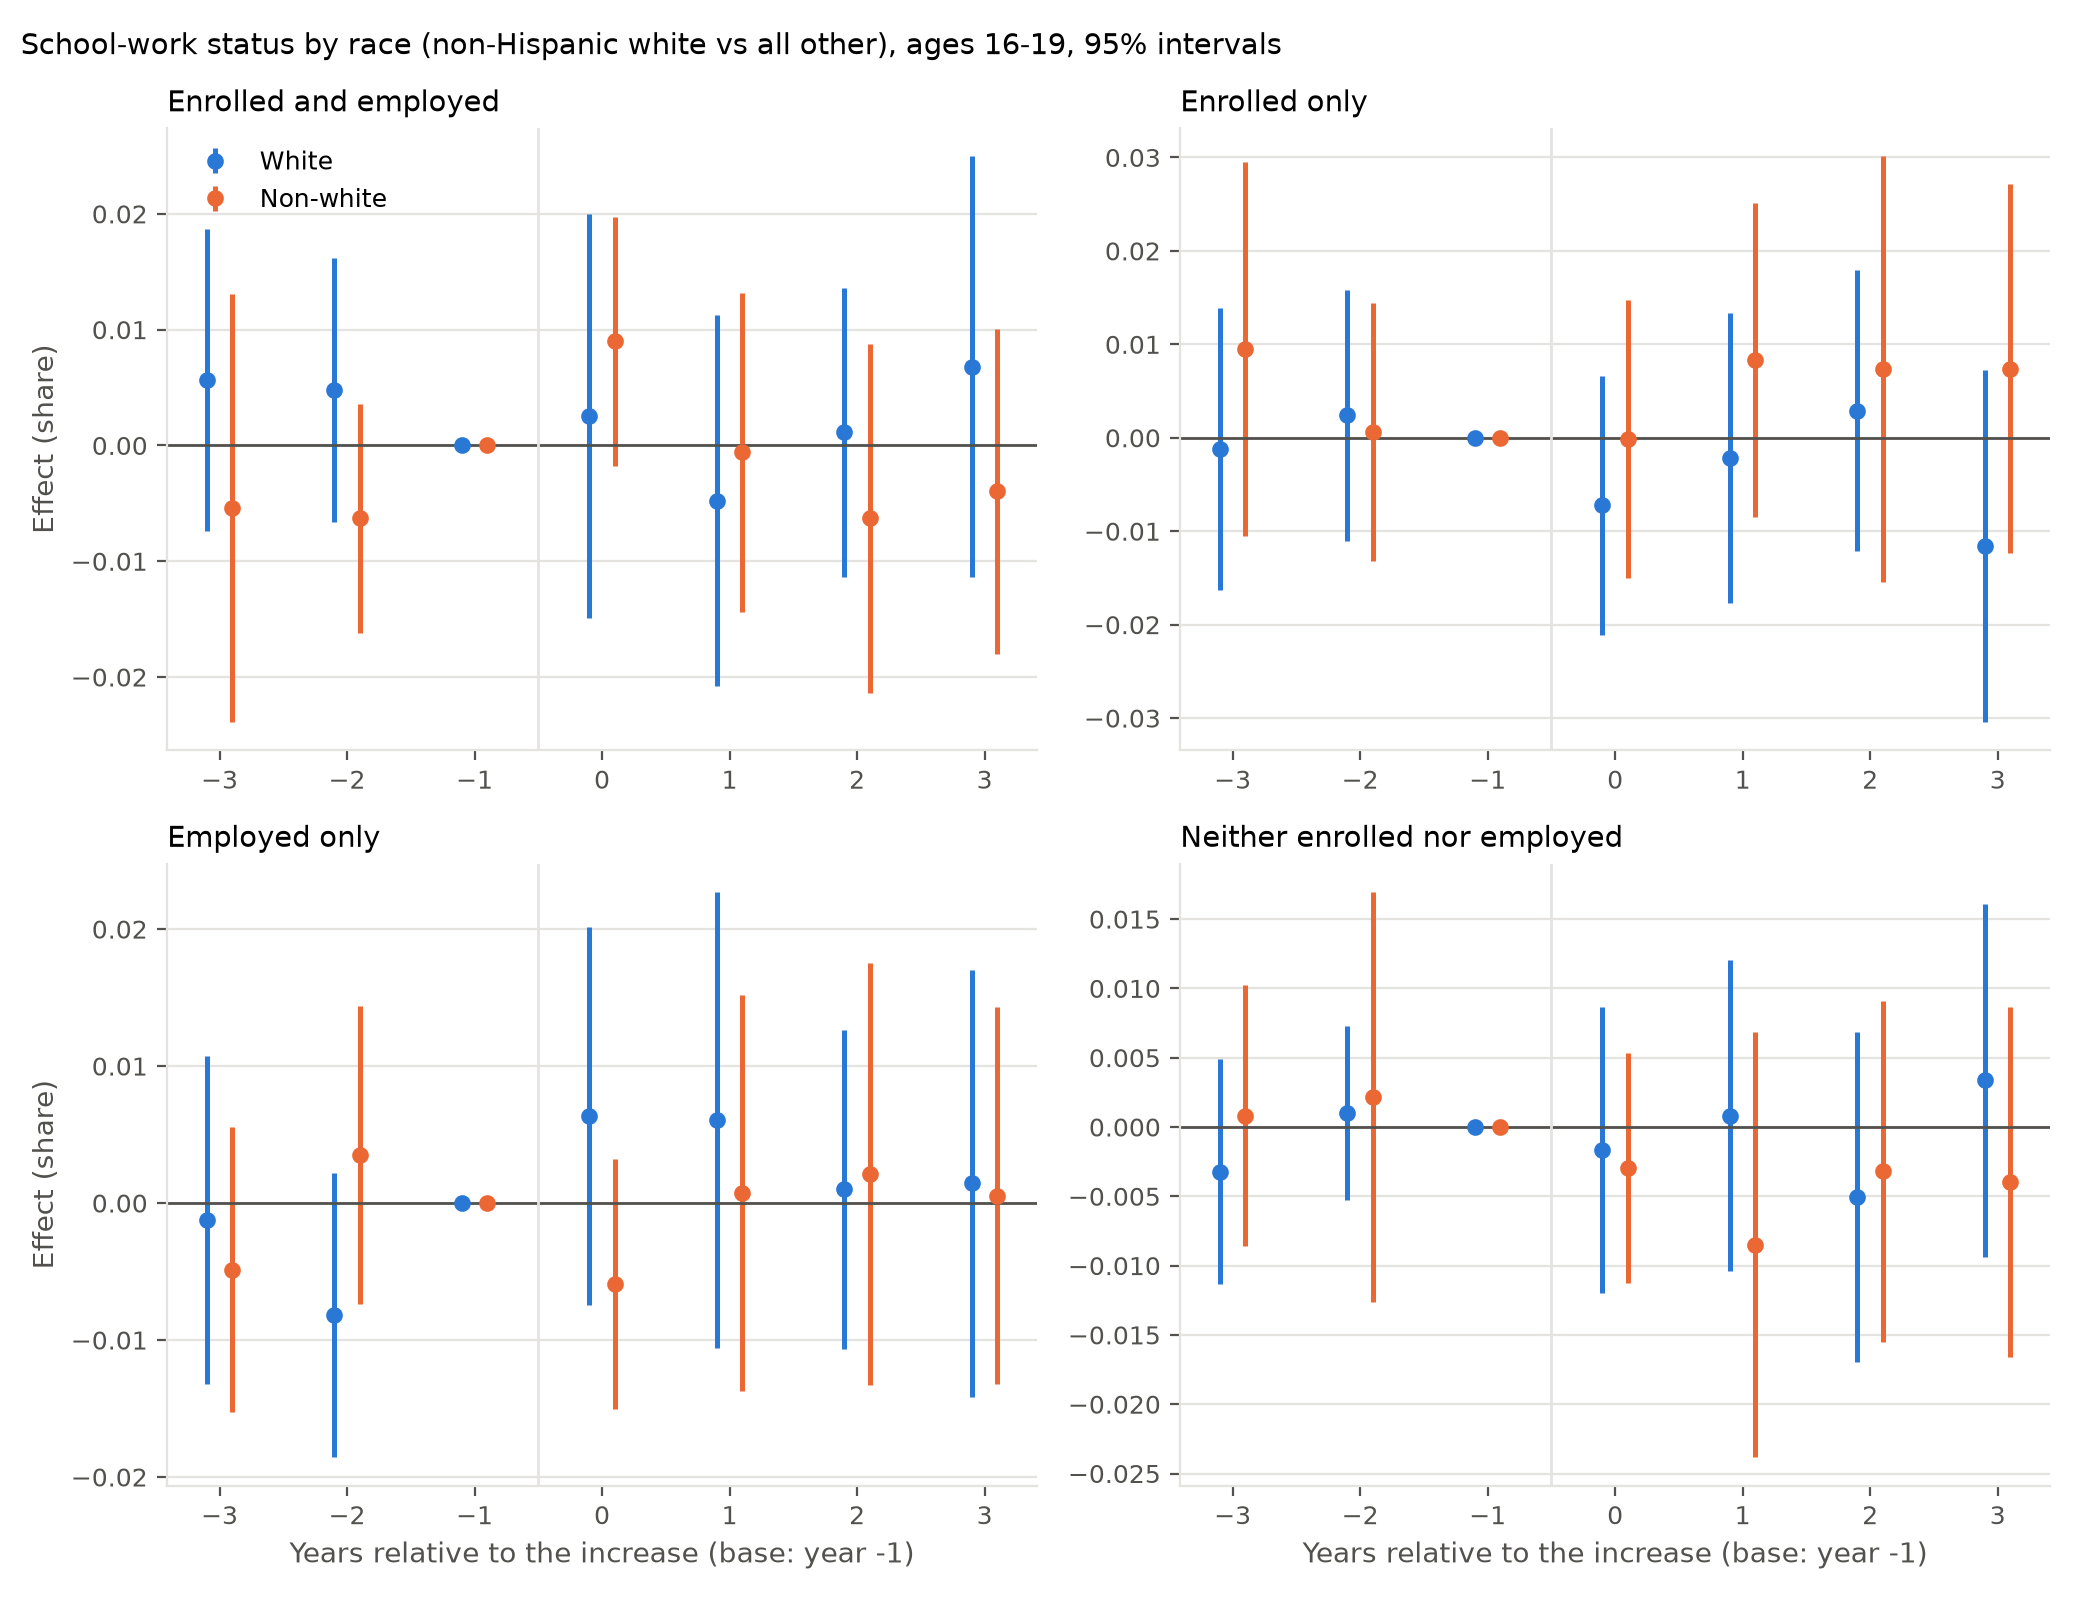
\includegraphics[width=\textwidth]{figures/figR2_groups_race.png}

\caption{Figure 6: Event-time effects on the four school--work shares by race, ages 16--19}

\end{figure}

\subsection{5.5 Wages}

Appendix Table 18 and Figure 7 give the effect on teen pay. Among hourly-paid teens in the outgoing rotation groups, the hourly wage in the event units rises relative to controls by 1.8 percent in the year of the increase, 6.8 percent in the first full year after it, 5.5 percent in the second and 7.0 percent in the third for 16--17 year olds, and by 0.7, 3.6, 2.8 and 5.0 percent for 18--19 year olds; pooling the ages, by 0.9, 4.6, 3.6 and 6.0 percent. The post-event averages are 5.3 percent (s.e.\ 1.2), 3.0 percent (0.9) and 3.8 percent (0.9). The year-0 effect is small because that year averages up to eleven pre-increase months with the first months after, and because most schedules add their later steps in years 1 to 3; from year 1 the wage effect is five to seven standard errors from zero and grows with the schedule. The pre-event coefficients are within about one standard error of zero. Weekly earnings of all teen workers, which combine the wage with hours, rise by 4.9 percent (3.2) at 16--17 and 4.2 percent (2.4) at 18--19, so hours did not fall to offset the wage.

The wage gain is about a seventh of the rise in the minimum. That is what one expects: a large share of hourly-paid teens already earn above the old minimum, the minimum binds most for the youngest and least experienced, and the hourly wage question is asked only of those paid by the hour. The point for the rest of the paper is that the events moved the pay of teenagers by an amount that is large relative to the precision of the time-allocation estimates, so the nulls of the previous two subsections are not nulls on the treatment.


The stacked coefficients for the wage (Table 6) are 5.1 percent (s.e.\ 0.8) at 16--17, 3.0 (0.8) at 18--19 and 3.8 (0.7) pooled, next to the event-study averages of 5.3, 3.0 and 3.8; for weekly earnings they are 5.2 (2.4), 4.4 (1.4) and 4.8 (1.7). The two-way fixed effects elasticity of the teen wage with respect to the minimum, in Appendix C, is about 0.2 at every age, which for the average event implies gains of 5 to 7 percent. Where the treatment has a real effect the designs agree in sign and roughly in size.

\begin{table}
\centering
\caption{Table 6: Stacked difference-in-differences estimates for teen wages and earnings, 73 events from 2010}

\small
\begin{tabular}{p{0.30\textwidth}p{0.227\textwidth}p{0.227\textwidth}p{0.227\textwidth}}
\toprule
 & Ages 16--17 & Ages 18--19 & Ages 16--19 \\
\midrule
Log hourly wage, hourly paid & 0.051\textsuperscript{***} & 0.030\textsuperscript{***} & 0.038\textsuperscript{***} \\
 & (0.008) & (0.008) & (0.007) \\
Log weekly earnings & 0.052\textsuperscript{**} & 0.044\textsuperscript{***} & 0.048\textsuperscript{***} \\
 & (0.024) & (0.014) & (0.017) \\
\bottomrule
\end{tabular}



\noindent\small Notes: Outgoing rotation groups, earnings weights. Specification as in Table 2; standard errors clustered by state in parentheses.

\end{table}

\begin{figure}
\centering

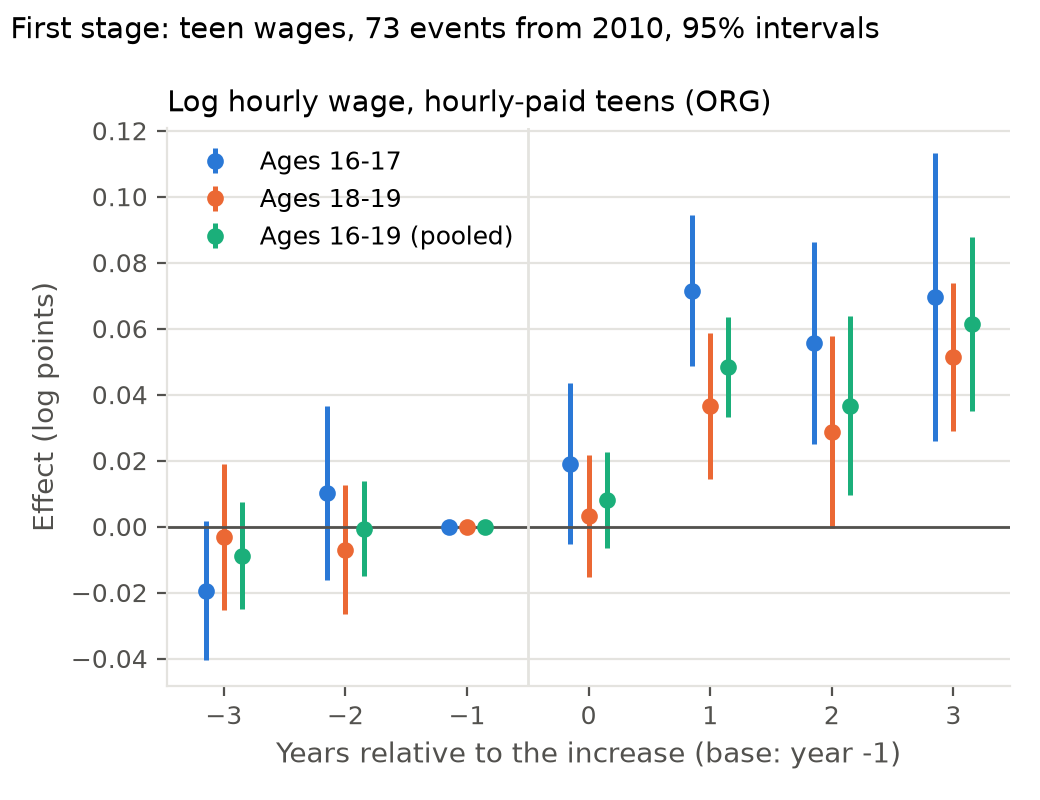
\includegraphics[width=0.85\textwidth]{figures/figR3_wage.png}

\caption{Figure 7: Event-time effects on the log hourly wage of hourly-paid teens, by age}

\end{figure}

\subsection{5.6 Wages by socioeconomic standing}

Table 7 and Figure 8 split the wage effect by family income. The gain reaches both groups. Pooling the ages, the hourly wage of low-income teens rises 4.4 percent (s.e.\ 1.1) and of high-income teens 3.6 percent (0.9). At 18--19 the gain is larger for low-income teens, 4.8 percent (1.2) against 2.3 (1.0), which is what one expects if their jobs sit closer to the floor. At 16--17 the low-income estimate is imprecise, 2.6 percent (2.7), because few low-income 16--17 year olds are hourly-paid workers in an outgoing rotation month; under the within-year median split of Appendix D it is 5.0 percent (1.9). The first stage is therefore present for exactly the teens for whom the liquidity channel should operate, and the previous subsections show that their time allocation did not respond to it.

\begin{table}
\centering
\caption{Table 7: Wages and earnings by family income: below versus at or above \$50,000, post-event averages}

\small
\begin{tabular}{p{0.30\textwidth}p{0.113\textwidth}p{0.113\textwidth}p{0.113\textwidth}p{0.113\textwidth}p{0.113\textwidth}p{0.113\textwidth}}
\toprule
 & \multicolumn{2}{c}{Ages 16--17} & \multicolumn{2}{c}{Ages 18--19} & \multicolumn{2}{c}{Ages 16--19} \\

 & Low & High & Low & High & Low & High \\
\midrule
Log hourly wage, hourly-paid teens & 0.026 & 0.058\textsuperscript{***} & 0.048\textsuperscript{***} & 0.023\textsuperscript{**} & 0.044\textsuperscript{***} & 0.036\textsuperscript{***} \\
 & (0.027) & (0.013) & (0.012) & (0.010) & (0.011) & (0.009) \\
Log weekly earnings, all teen workers &  &  &  &  &  &  \\
 &  &  &  &  &  &  \\
\bottomrule
\end{tabular}



\noindent\small Notes: Outgoing rotation groups, earnings weights. Block-bootstrap standard errors in parentheses.

\end{table}

The stacked coefficients by income (Table 8) confirm that the gain reached both groups and was somewhat larger for the poorer one. Because the stacked regression pools the base period over 36 months, it is more precise than the event-study average for the thin low-income 16--17 cell: it gives 7.7 percent (s.e.\ 1.3) for low-income against 4.4 (0.9) for high-income teens at 16--17, 4.1 (1.1) against 2.3 (0.9) at 18--19, and 5.1 (1.1) against 3.2 (0.8) pooled.

\begin{table}
\centering
\caption{Table 8: Stacked difference-in-differences estimates for wages and earnings by family income}

\small
\begin{tabular}{p{0.30\textwidth}p{0.113\textwidth}p{0.113\textwidth}p{0.113\textwidth}p{0.113\textwidth}p{0.113\textwidth}p{0.113\textwidth}}
\toprule
 & \multicolumn{2}{c}{Ages 16--17} & \multicolumn{2}{c}{Ages 18--19} & \multicolumn{2}{c}{Ages 16--19} \\

 & Low & High & Low & High & Low & High \\
\midrule
Log hourly wage, hourly paid & 0.077\textsuperscript{***} & 0.044\textsuperscript{***} & 0.041\textsuperscript{***} & 0.023\textsuperscript{**} & 0.051\textsuperscript{***} & 0.032\textsuperscript{***} \\
 & (0.013) & (0.009) & (0.011) & (0.009) & (0.011) & (0.008) \\
Log weekly earnings & 0.064\textsuperscript{*} & 0.060\textsuperscript{**} & 0.045 & 0.035\textsuperscript{**} & 0.051\textsuperscript{**} & 0.045\textsuperscript{***} \\
 & (0.036) & (0.025) & (0.029) & (0.015) & (0.026) & (0.017) \\
\bottomrule
\end{tabular}



\noindent\small Notes: Low: family income below \$50,000; High: \$50,000 or more. Outgoing rotation groups, earnings weights. Specification as in Table 2; standard errors clustered by state in parentheses.

\end{table}

\begin{figure}
\centering

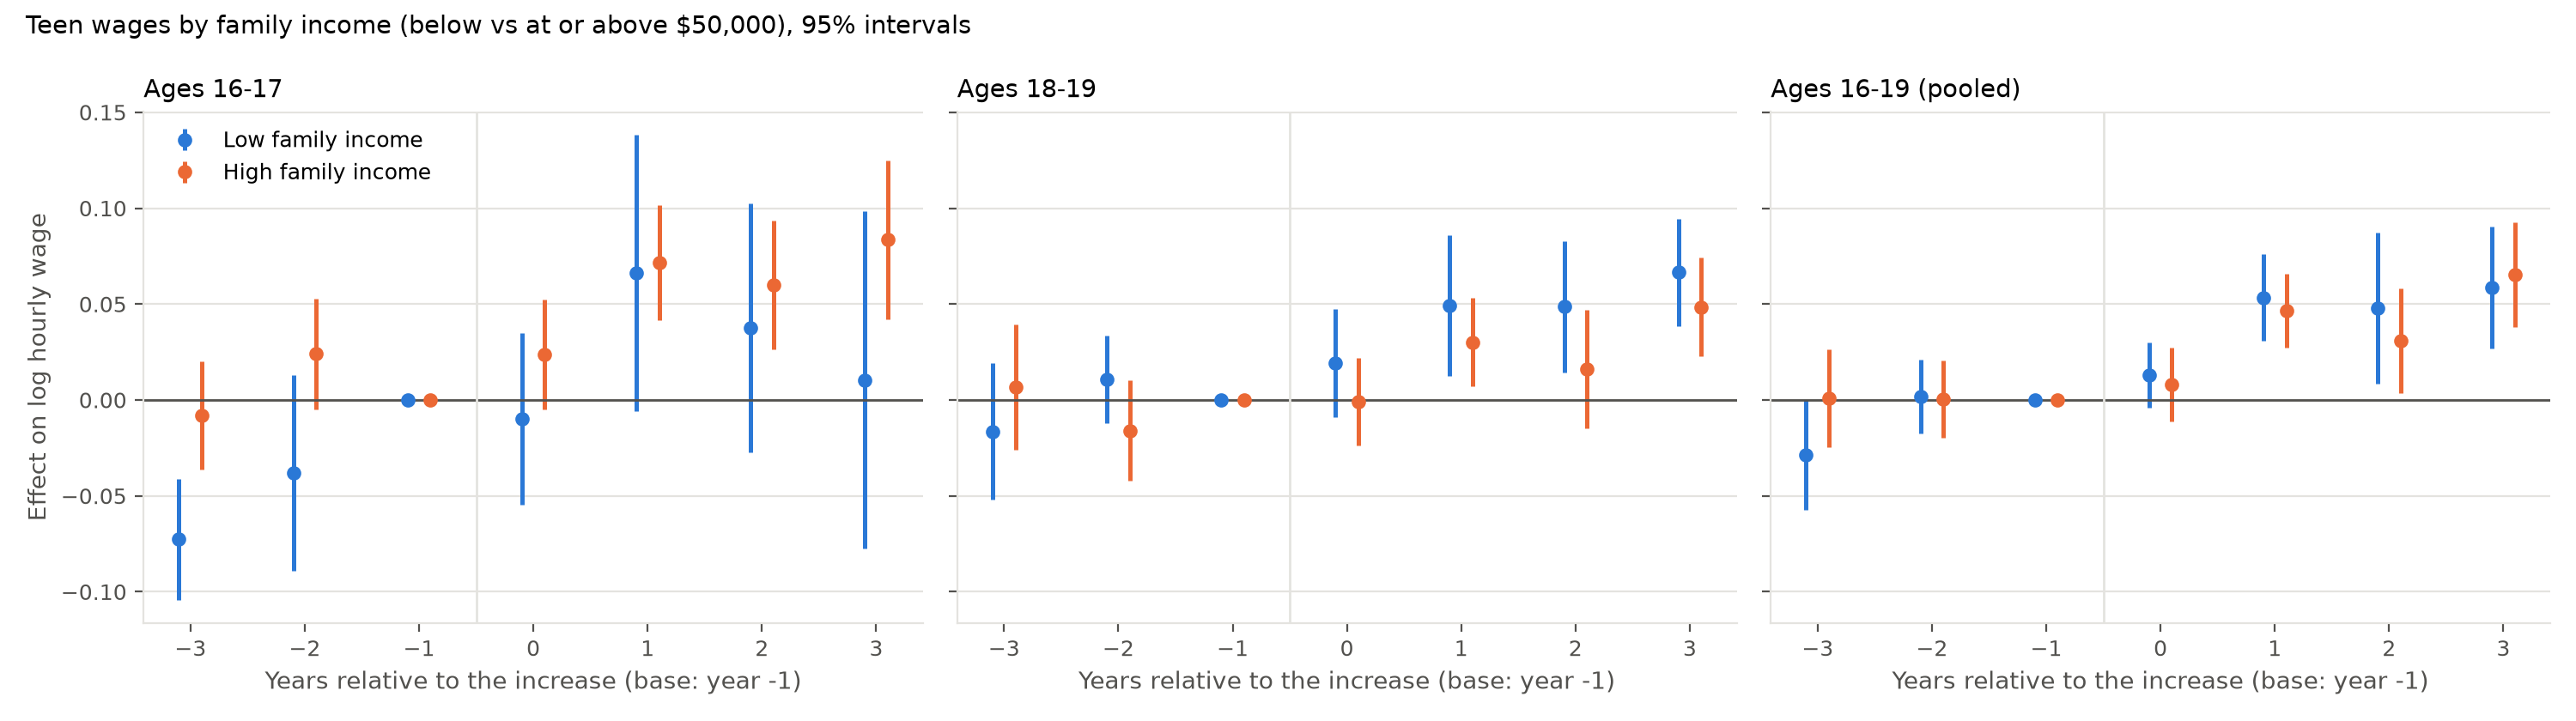
\includegraphics[width=\textwidth]{figures/figR4_wage_ses.png}

\caption{Figure 8: Event-time effects on the log hourly wage by family income and age}

\end{figure}

\subsection{5.7 Wages by sex}

Table 9 and Figure 9 split the wage effect by sex. The gain reaches both. Girls' hourly wage rises 5.4 percent (s.e.\ 1.9) at 16--17, 3.4 (0.9) at 18--19 and 4.1 (1.0) pooled; boys' 4.7 (1.7), 2.5 (1.4) and 3.5 (1.2). The girls' gain is larger at every age, as their lower starting wage implies, but by less than a standard error, and by the third year after the increase both are at about 6 percent. Weekly earnings rise 5.5 (3.2) at 16--17 and 4.5 (2.6) at 18--19 for girls and 5.4 (4.8) and 3.7 (3.4) for boys, so hours did not fall for either. The employment estimate for girls at 16--17 in Section 5.3 therefore does not come with a smaller wage gain or a fall in the earnings of those who work. The stacked coefficients (Table 10) are 5.5 percent (s.e.\ 1.2), 2.6 (0.8) and 3.8 (0.8) for girls and 4.8 (0.9), 3.5 (1.0) and 4.1 (0.8) for boys.

\begin{table}
\centering
\caption{Table 9: Wages and earnings by sex: post-event averages}

\small
\begin{tabular}{p{0.30\textwidth}p{0.113\textwidth}p{0.113\textwidth}p{0.113\textwidth}p{0.113\textwidth}p{0.113\textwidth}p{0.113\textwidth}}
\toprule
 & \multicolumn{2}{c}{Ages 16--17} & \multicolumn{2}{c}{Ages 18--19} & \multicolumn{2}{c}{Ages 16--19} \\

 & Girls & Boys & Girls & Boys & Girls & Boys \\
\midrule
Log hourly wage, hourly-paid teens & 0.054\textsuperscript{***} & 0.047\textsuperscript{***} & 0.034\textsuperscript{***} & 0.025\textsuperscript{*} & 0.041\textsuperscript{***} & 0.035\textsuperscript{***} \\
 & (0.019) & (0.017) & (0.009) & (0.014) & (0.010) & (0.012) \\
Log weekly earnings, all teen workers & 0.055\textsuperscript{*} & 0.054 & 0.045\textsuperscript{*} & 0.037 & 0.043\textsuperscript{*} & 0.041 \\
 & (0.032) & (0.048) & (0.026) & (0.034) & (0.022) & (0.036) \\
\bottomrule
\end{tabular}



\noindent\small Notes: Outgoing rotation groups, earnings weights. Block-bootstrap standard errors in parentheses.

\end{table}

\begin{table}
\centering
\caption{Table 10: Stacked difference-in-differences estimates for wages and earnings by sex}

\small
\begin{tabular}{p{0.30\textwidth}p{0.113\textwidth}p{0.113\textwidth}p{0.113\textwidth}p{0.113\textwidth}p{0.113\textwidth}p{0.113\textwidth}}
\toprule
 & \multicolumn{2}{c}{Ages 16--17} & \multicolumn{2}{c}{Ages 18--19} & \multicolumn{2}{c}{Ages 16--19} \\

 & Girls & Boys & Girls & Boys & Girls & Boys \\
\midrule
Log hourly wage, hourly paid & 0.055\textsuperscript{***} & 0.048\textsuperscript{***} & 0.026\textsuperscript{***} & 0.035\textsuperscript{***} & 0.038\textsuperscript{***} & 0.041\textsuperscript{***} \\
 & (0.012) & (0.009) & (0.008) & (0.010) & (0.008) & (0.008) \\
Log weekly earnings & 0.047 & 0.056\textsuperscript{*} & 0.050\textsuperscript{***} & 0.042\textsuperscript{**} & 0.050\textsuperscript{**} & 0.051\textsuperscript{**} \\
 & (0.031) & (0.032) & (0.018) & (0.018) & (0.020) & (0.020) \\
\bottomrule
\end{tabular}



\noindent\small Notes: Outgoing rotation groups, earnings weights. Specification as in Table 2; standard errors clustered by state in parentheses.

\end{table}

\begin{figure}
\centering

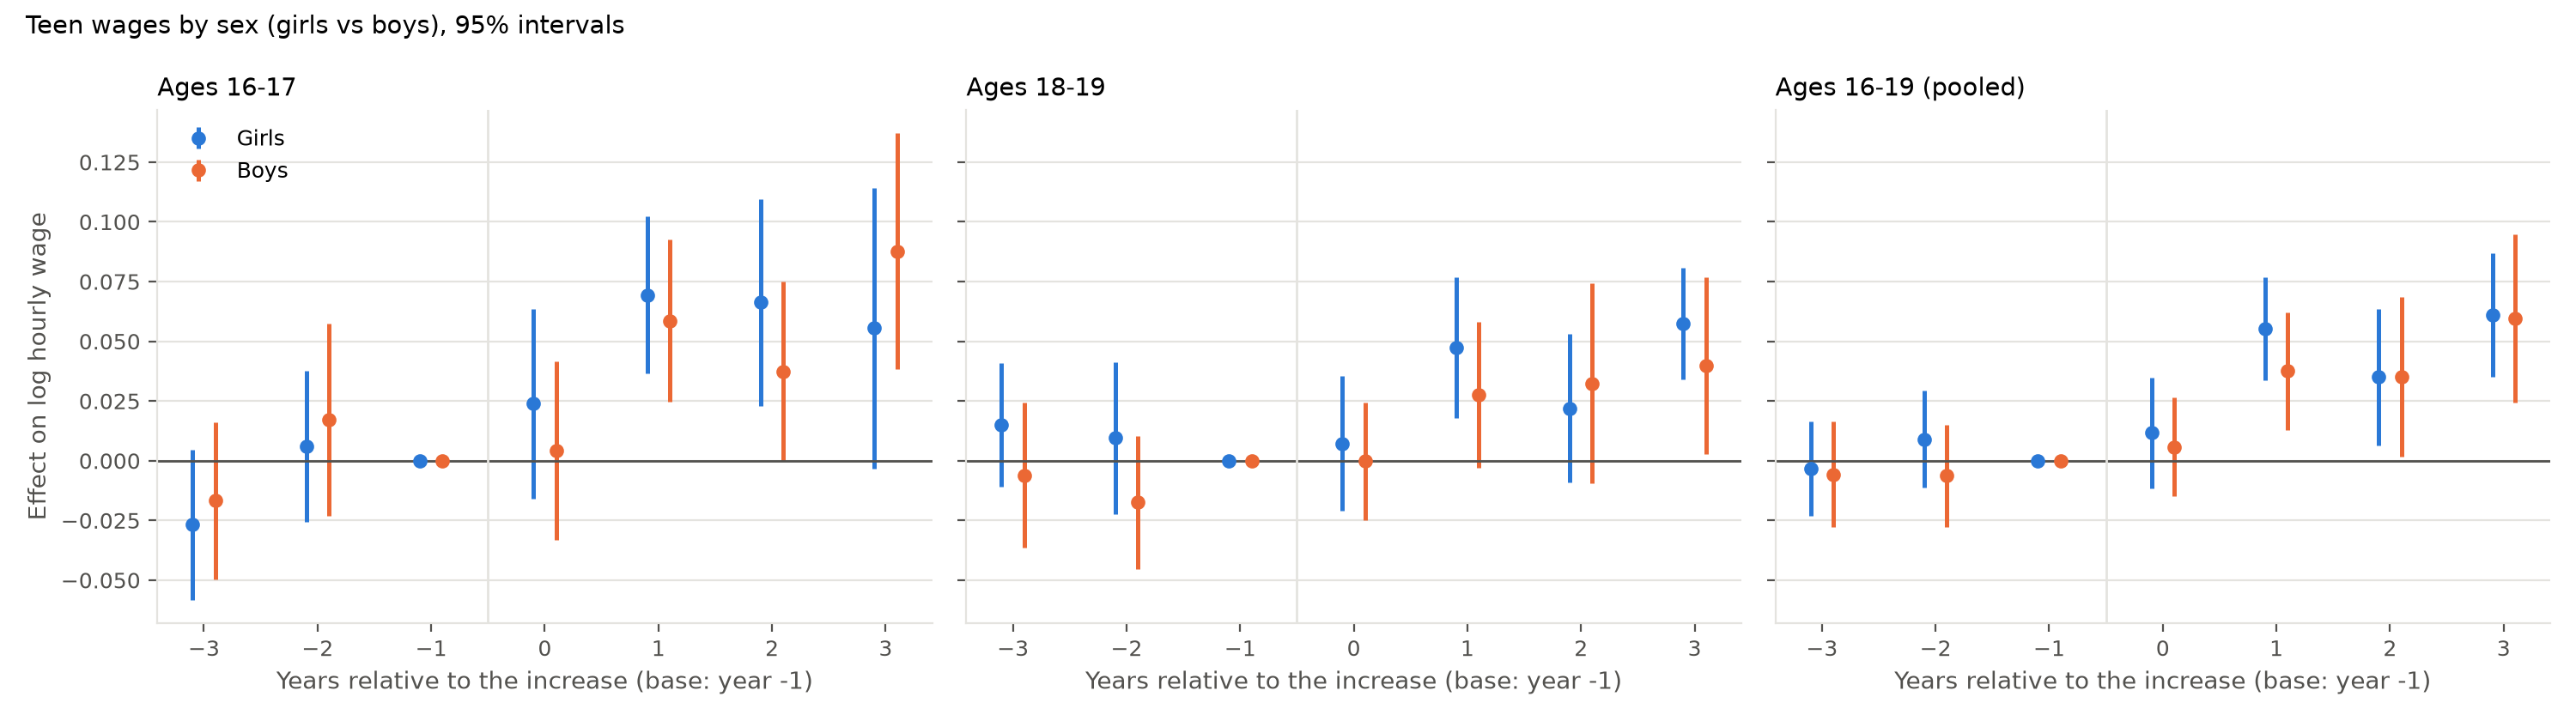
\includegraphics[width=\textwidth]{figures/figR4_wage_sex.png}

\caption{Figure 9: Event-time effects on the log hourly wage by sex and age}

\end{figure}

\subsection{5.8 Wages by race}

Table 11 and Figure 10 split the wage effect by race. Non-white teens gain more: 7.4 percent (s.e.\ 1.6) at 16--17 against 4.9 (1.8) for white teens, 3.5 (1.4) against 2.8 (1.3) at 18--19, and 4.3 (1.2) against 3.6 (1.3) pooled. The 2.5-point difference at 16--17 is what one expects if non-white teens' jobs sit closer to the floor and if they are concentrated in the units with the largest increases. Weekly earnings of non-white teen workers are too thinly measured to say much, $+4.7$ (7.4) at 16--17 and $+3.1$ (3.8) at 18--19, against $+5.8$ (3.3) and $+6.0$ (3.1) for white teens. The first stage is present, and larger, for the group whose families have lower incomes, and Section 5.4 shows that their time allocation did not respond to it. The stacked coefficients (Table 12) are 4.8 percent (s.e.\ 1.1), 2.5 (1.2) and 3.5 (0.9) for white teens and 6.1 (1.2), 3.8 (1.1) and 4.5 (0.9) for non-white teens.

\begin{table}
\centering
\caption{Table 11: Wages and earnings by race: post-event averages}

\small
\begin{tabular}{p{0.30\textwidth}p{0.113\textwidth}p{0.113\textwidth}p{0.113\textwidth}p{0.113\textwidth}p{0.113\textwidth}p{0.113\textwidth}}
\toprule
 & \multicolumn{2}{c}{Ages 16--17} & \multicolumn{2}{c}{Ages 18--19} & \multicolumn{2}{c}{Ages 16--19} \\

 & White & Non-white & White & Non-white & White & Non-white \\
\midrule
Log hourly wage, hourly-paid teens & 0.049\textsuperscript{***} & 0.074\textsuperscript{***} & 0.028\textsuperscript{**} & 0.035\textsuperscript{***} & 0.036\textsuperscript{***} & 0.043\textsuperscript{***} \\
 & (0.018) & (0.016) & (0.013) & (0.014) & (0.013) & (0.012) \\
Log weekly earnings, all teen workers & 0.058\textsuperscript{*} & 0.047 & 0.060\textsuperscript{*} & 0.031 & 0.060\textsuperscript{**} & 0.029 \\
 & (0.033) & (0.074) & (0.031) & (0.038) & (0.026) & (0.039) \\
\bottomrule
\end{tabular}



\noindent\small Notes: White: non-Hispanic white; Non-white: Black, Hispanic and other. Outgoing rotation groups, earnings weights. Block-bootstrap standard errors in parentheses.

\end{table}

\begin{table}
\centering
\caption{Table 12: Stacked difference-in-differences estimates for wages and earnings by race}

\small
\begin{tabular}{p{0.30\textwidth}p{0.113\textwidth}p{0.113\textwidth}p{0.113\textwidth}p{0.113\textwidth}p{0.113\textwidth}p{0.113\textwidth}}
\toprule
 & \multicolumn{2}{c}{Ages 16--17} & \multicolumn{2}{c}{Ages 18--19} & \multicolumn{2}{c}{Ages 16--19} \\

 & White & Non-white & White & Non-white & White & Non-white \\
\midrule
Log hourly wage, hourly paid & 0.048\textsuperscript{***} & 0.061\textsuperscript{***} & 0.025\textsuperscript{**} & 0.038\textsuperscript{***} & 0.035\textsuperscript{***} & 0.045\textsuperscript{***} \\
 & (0.011) & (0.012) & (0.012) & (0.011) & (0.009) & (0.009) \\
Log weekly earnings & 0.050\textsuperscript{**} & 0.070\textsuperscript{*} & 0.051\textsuperscript{**} & 0.035 & 0.052\textsuperscript{***} & 0.041\textsuperscript{*} \\
 & (0.023) & (0.037) & (0.020) & (0.024) & (0.018) & (0.024) \\
\bottomrule
\end{tabular}



\noindent\small Notes: White: non-Hispanic white; Non-white: Black, Hispanic and other. Outgoing rotation groups, earnings weights. Specification as in Table 2; standard errors clustered by state in parentheses.

\end{table}

\begin{figure}
\centering

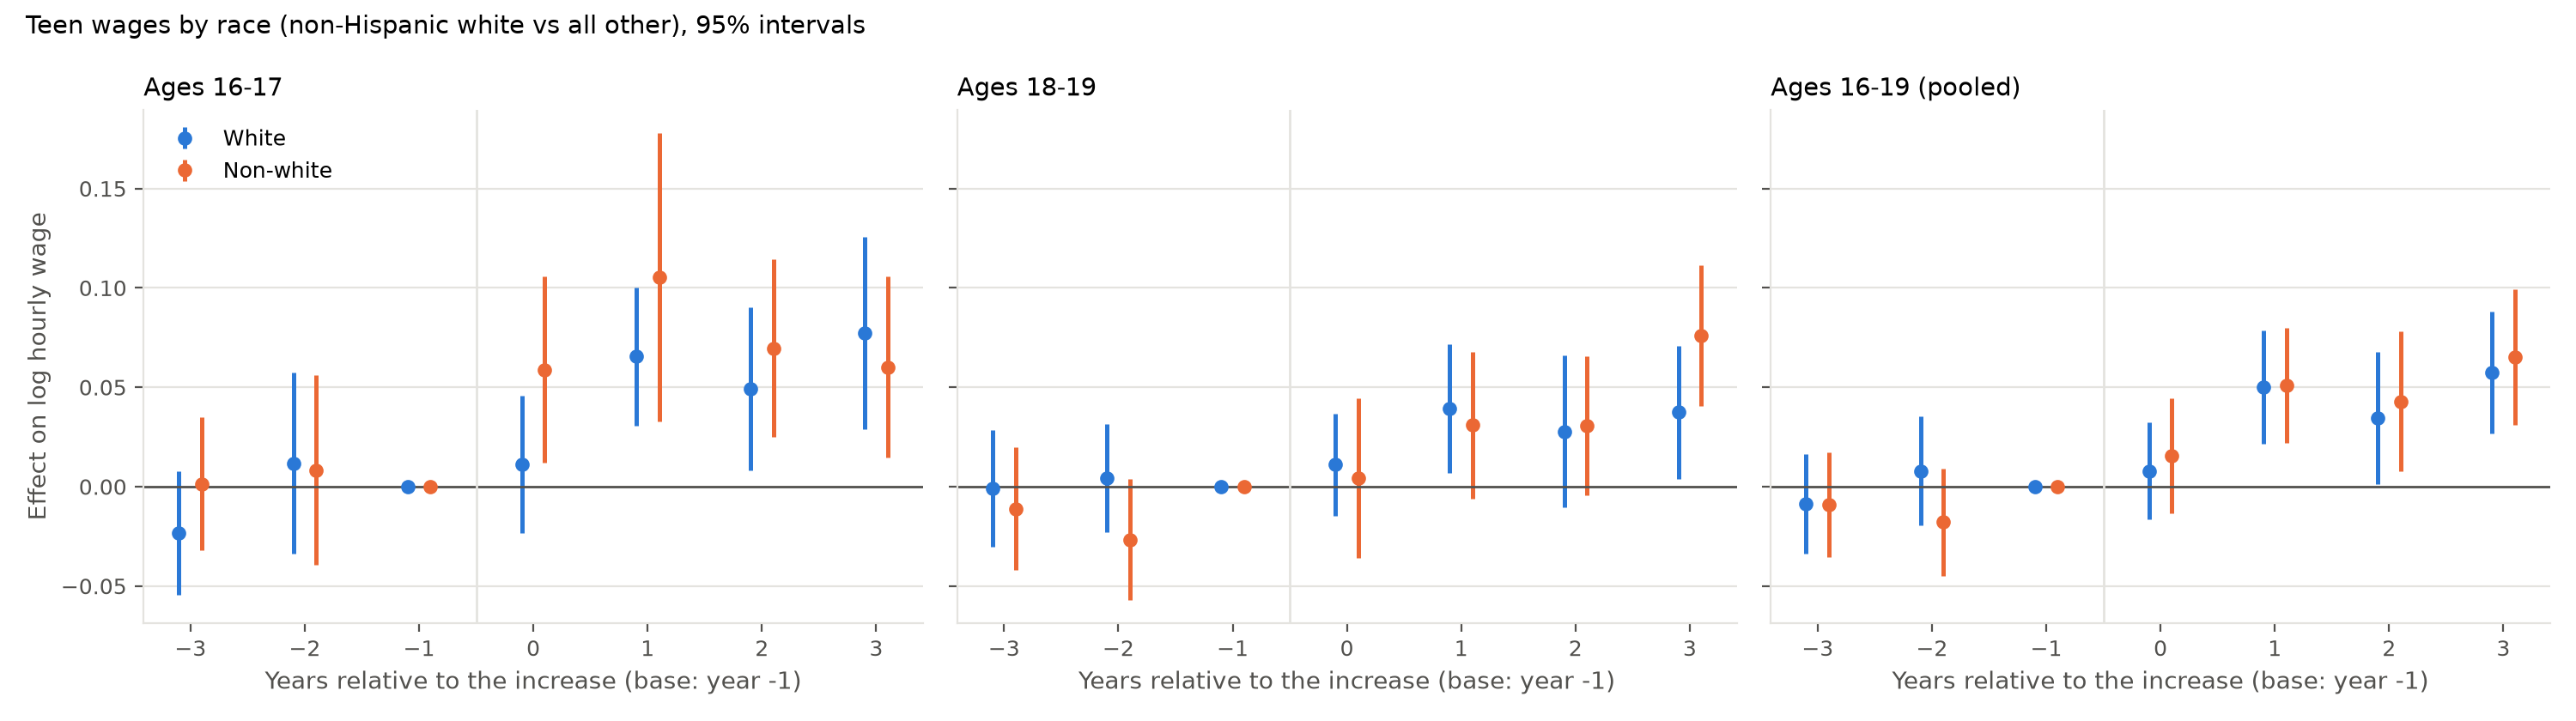
\includegraphics[width=\textwidth]{figures/figR4_wage_race.png}

\caption{Figure 10: Event-time effects on the log hourly wage by race and age}

\end{figure}

\section{6 Robustness}

Table 13 re-estimates the enrollment, employment and neither-enrolled-nor-employed effects under alternative units, event sets, control sets, weights and samples. Treating states as the units, so that a county's local minimum is ignored and its teens are counted at the state rate, gives enrollment effects of $-0.3$ (s.e.\ 0.4) and $-0.4$ (s.e.\ 0.9) from 39 state events, the same as the unit design; Figures 11 and 12 are the state-design counterparts of the main figures. Within the unit design, the 39 state-remainder events alone give $-0.5$ (0.5) and $-0.9$ (1.0). The 62 events with a window rise of at least 20 percent give $-0.2$ and $-0.0$. Restricting controls to units with no increase of any kind or to the states at the federal floor, dropping 2020 and 2021, and using September to May only all leave the estimates within one standard error of zero. Equal weighting of events gives $+0.3$ (0.5) and $+1.8$ (0.9) at 18--19, the latter with a pre-event average of $+2.1$, because equal weights give the small county units, whose enrollment was already rising, the same weight as California. No employment estimate in the table is more than one standard error below zero. Ages 20--24 show $-0.2$ (s.e.\ 0.7) on enrollment and $+0.1$ (s.e.\ 0.5) on employment.

The county events deserve a word. Their first stage is larger, 8.5 percent (s.e.\ 4.4) at 16--17 for the local-only events, because local increases were larger. Their enrollment estimates at 18--19 are positive: $+3.3$ points (s.e.\ 0.9) for the 18 county events with both a state and a local rise and $+7.5$ (3.4) for the 16 local-only events. Their pre-event averages are positive as well, $+1.3$ and $+5.3$: enrollment of 18--19 year olds in the big-city counties was rising relative to other states' units before the increases. Net of the pre-event trend the post-event change is about two points in both sets, with county samples of 13 to 40 teens a month. The aggregate estimates, in which these events carry a fifth of the weight, are unaffected by them. Figure 13 shows the event-by-event enrollment estimates at 18--19: 30 of the 73 are negative and 43 positive, and no single event or unit drives the aggregate. Table 14 lists the event-time coefficients behind the main figures.

\begin{table}
\centering
\caption{Table 13: Robustness: post-event averages under alternative units, event sets, controls, weights and samples}

\footnotesize
\begin{tabular}{p{0.30\textwidth}p{0.085\textwidth}p{0.085\textwidth}p{0.085\textwidth}p{0.085\textwidth}p{0.085\textwidth}p{0.085\textwidth}p{0.085\textwidth}p{0.085\textwidth}}
\toprule
 & \multicolumn{2}{c}{Enrolled} & \multicolumn{2}{c}{Employed} & \multicolumn{2}{c}{Neither} & Events \\

 & 16--17 & 18--19 & 16--17 & 18--19 & 16--17 & 18--19 & \\
\midrule
Main: unit design, 73 events from 2010, clean controls, population weights & -0.003 & 0.001 & -0.001 & 0.010 & 0.001 & -0.005 & 73 \\
 & (0.004) & (0.009) & (0.005) & (0.007) & (0.004) & (0.005) &  \\
State design (states as units), 39 events (Appendix) & -0.003 & -0.004 & -0.000 & 0.013 & 0.001 & -0.003 & 39 \\
 & (0.004) & (0.009) & (0.005) & (0.008) & (0.003) & (0.006) &  \\
Unit design: state-remainder events only (39) & -0.005 & -0.009 & 0.004 & 0.015\textsuperscript{*} &  &  & 39 \\
 & (0.005) & (0.010) & (0.005) & (0.008) &  &  &  \\
Unit design: county events, state and local rise (18) & 0.005 & 0.033\textsuperscript{***} & -0.021 & 0.003 &  &  & 18 \\
 & (0.007) & (0.009) & (0.029) & (0.023) &  &  &  \\
Unit design: county events, local rise only (16) & 0.016 & 0.075\textsuperscript{**} & -0.016 & -0.047 &  &  & 16 \\
 & (0.017) & (0.034) & (0.028) & (0.051) &  &  &  \\
Large events only (window rise $\geq$ 20\%) & -0.002 & -0.000 & -0.002 & 0.014\textsuperscript{*} & 0.001 & -0.005 & 62 \\
 & (0.004) & (0.010) & (0.005) & (0.007) & (0.004) & (0.005) &  \\
Strict controls (no rise of any kind) & -0.003 & 0.001 & -0.001 & 0.010 & 0.001 & -0.005 & 73 \\
 & (0.004) & (0.009) & (0.005) & (0.007) & (0.004) & (0.005) &  \\
Federal-floor controls only & -0.003 & -0.001 & -0.003 & 0.011 & 0.002 & -0.002 & 73 \\
 & (0.004) & (0.009) & (0.005) & (0.008) & (0.004) & (0.006) &  \\
Equal weight per event & 0.003 & 0.018\textsuperscript{*} & -0.004 & -0.003 & -0.000 & -0.008 & 73 \\
 & (0.005) & (0.009) & (0.007) & (0.010) & (0.004) & (0.006) &  \\
Drop 2020--21 & -0.002 & 0.001 & -0.001 & 0.012 & -0.001 & -0.005 & 62 \\
 & (0.003) & (0.009) & (0.005) & (0.010) & (0.003) & (0.006) &  \\
September--May only & -0.006 & -0.002 & 0.001 & 0.011 & 0.004 & -0.003 & 73 \\
 & (0.004) & (0.007) & (0.006) & (0.008) & (0.002) & (0.006) &  \\
\bottomrule
\end{tabular}



\noindent\small Notes: Each cell is the post-event average effect on the outcome for the age group; block-bootstrap standard errors in parentheses. Events: number of events in the specification.

\end{table}

\begin{table}
\centering
\caption{Table 14: Event-time coefficients: log hourly wage, enrollment and employment, 73 events from 2010}

\small
\begin{tabular}{p{0.30\textwidth}p{0.113\textwidth}p{0.113\textwidth}p{0.113\textwidth}p{0.113\textwidth}p{0.113\textwidth}p{0.113\textwidth}}
\toprule
 & \multicolumn{2}{c}{Log hourly wage} & \multicolumn{2}{c}{Enrolled} & \multicolumn{2}{c}{Employed} \\

 & 16--17 & 18--19 & 16--17 & 18--19 & 16--17 & 18--19 \\
\midrule
Year -3 & -0.021\textsuperscript{**} & 0.004 & -0.000 & 0.007 & -0.005 & -0.002 \\
 & (0.010) & (0.013) & (0.004) & (0.009) & (0.007) & (0.009) \\
Year -2 & 0.010 & -0.004 & -0.002 & 0.004 & -0.002 & -0.003 \\
 & (0.013) & (0.009) & (0.003) & (0.008) & (0.006) & (0.007) \\
Year -1 & 0 & 0 & 0 & 0 & 0 & 0 \\
 &  &  &  &  &  &  \\
Year 0 & 0.018 & 0.007 & -0.003 & 0.004 & -0.000 & 0.012\textsuperscript{*} \\
 & (0.012) & (0.010) & (0.004) & (0.010) & (0.006) & (0.007) \\
Year 1 & 0.068\textsuperscript{***} & 0.036\textsuperscript{***} & -0.004 & -0.002 & -0.001 & 0.009 \\
 & (0.011) & (0.011) & (0.007) & (0.009) & (0.006) & (0.012) \\
Year 2 & 0.055\textsuperscript{***} & 0.028\textsuperscript{*} & -0.003 & 0.006 & 0.002 & 0.002 \\
 & (0.015) & (0.015) & (0.006) & (0.009) & (0.007) & (0.009) \\
Year 3 & 0.070\textsuperscript{***} & 0.050\textsuperscript{***} & -0.002 & -0.003 & -0.004 & 0.017 \\
 & (0.021) & (0.011) & (0.006) & (0.013) & (0.009) & (0.010) \\
\bottomrule
\end{tabular}



\noindent\small Notes: Relative year $-1$ is the twelve months before the increase and the omitted base. Block-bootstrap standard errors over states in parentheses.

\end{table}

\begin{figure}
\centering

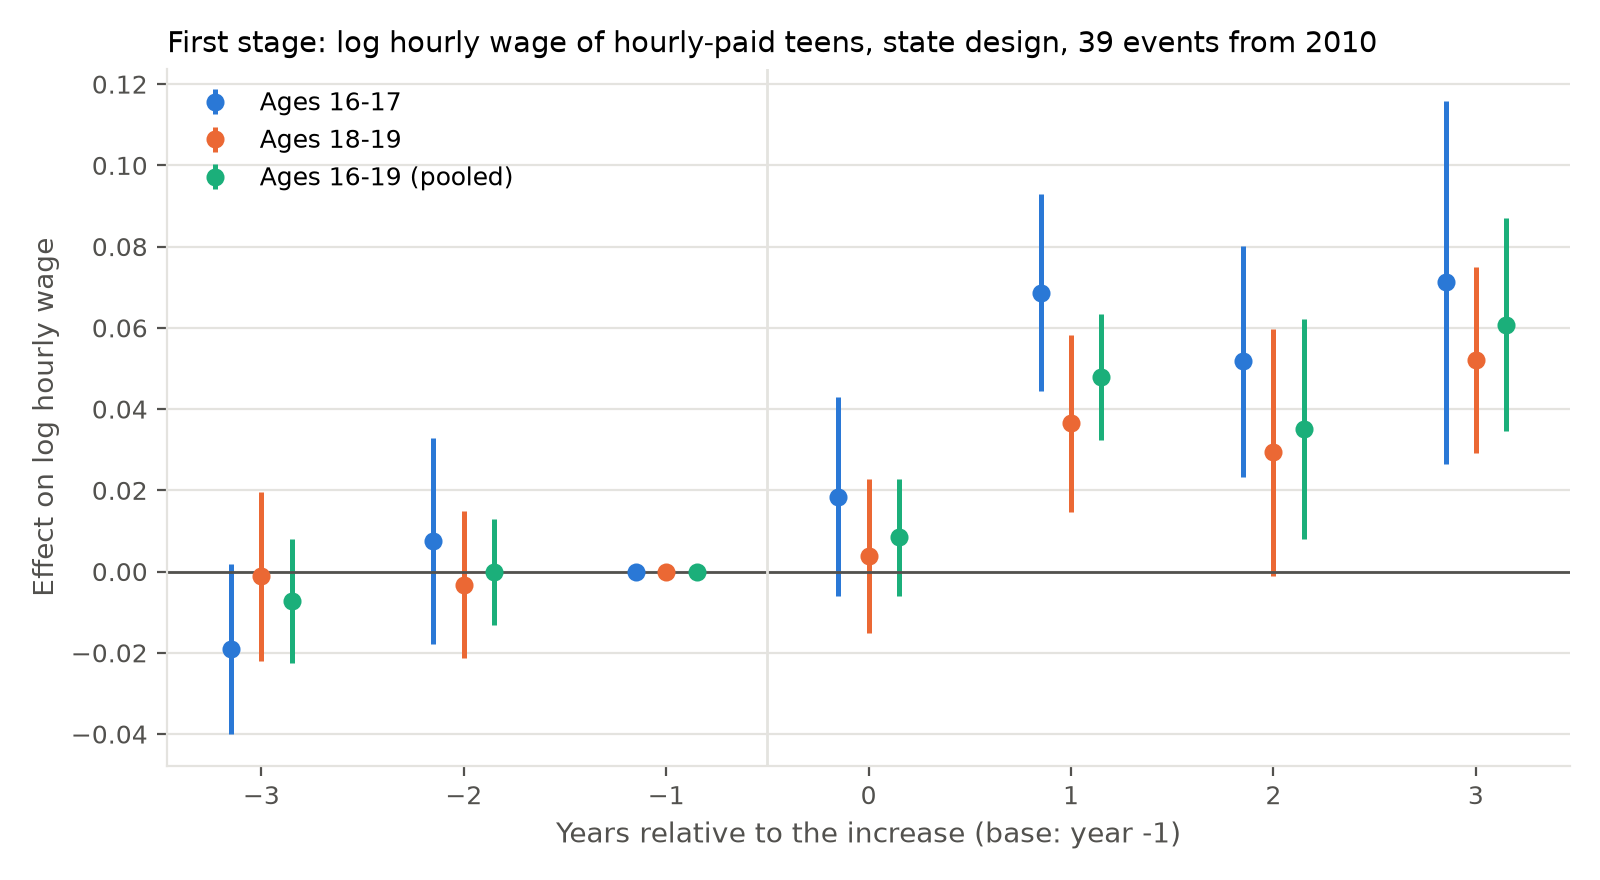
\includegraphics[width=0.85\textwidth]{figures/figA1_state_first_stage.png}

\caption{Figure 11: State design (states as units, 39 events from 2010): first stage}

\end{figure}

\begin{figure}
\centering

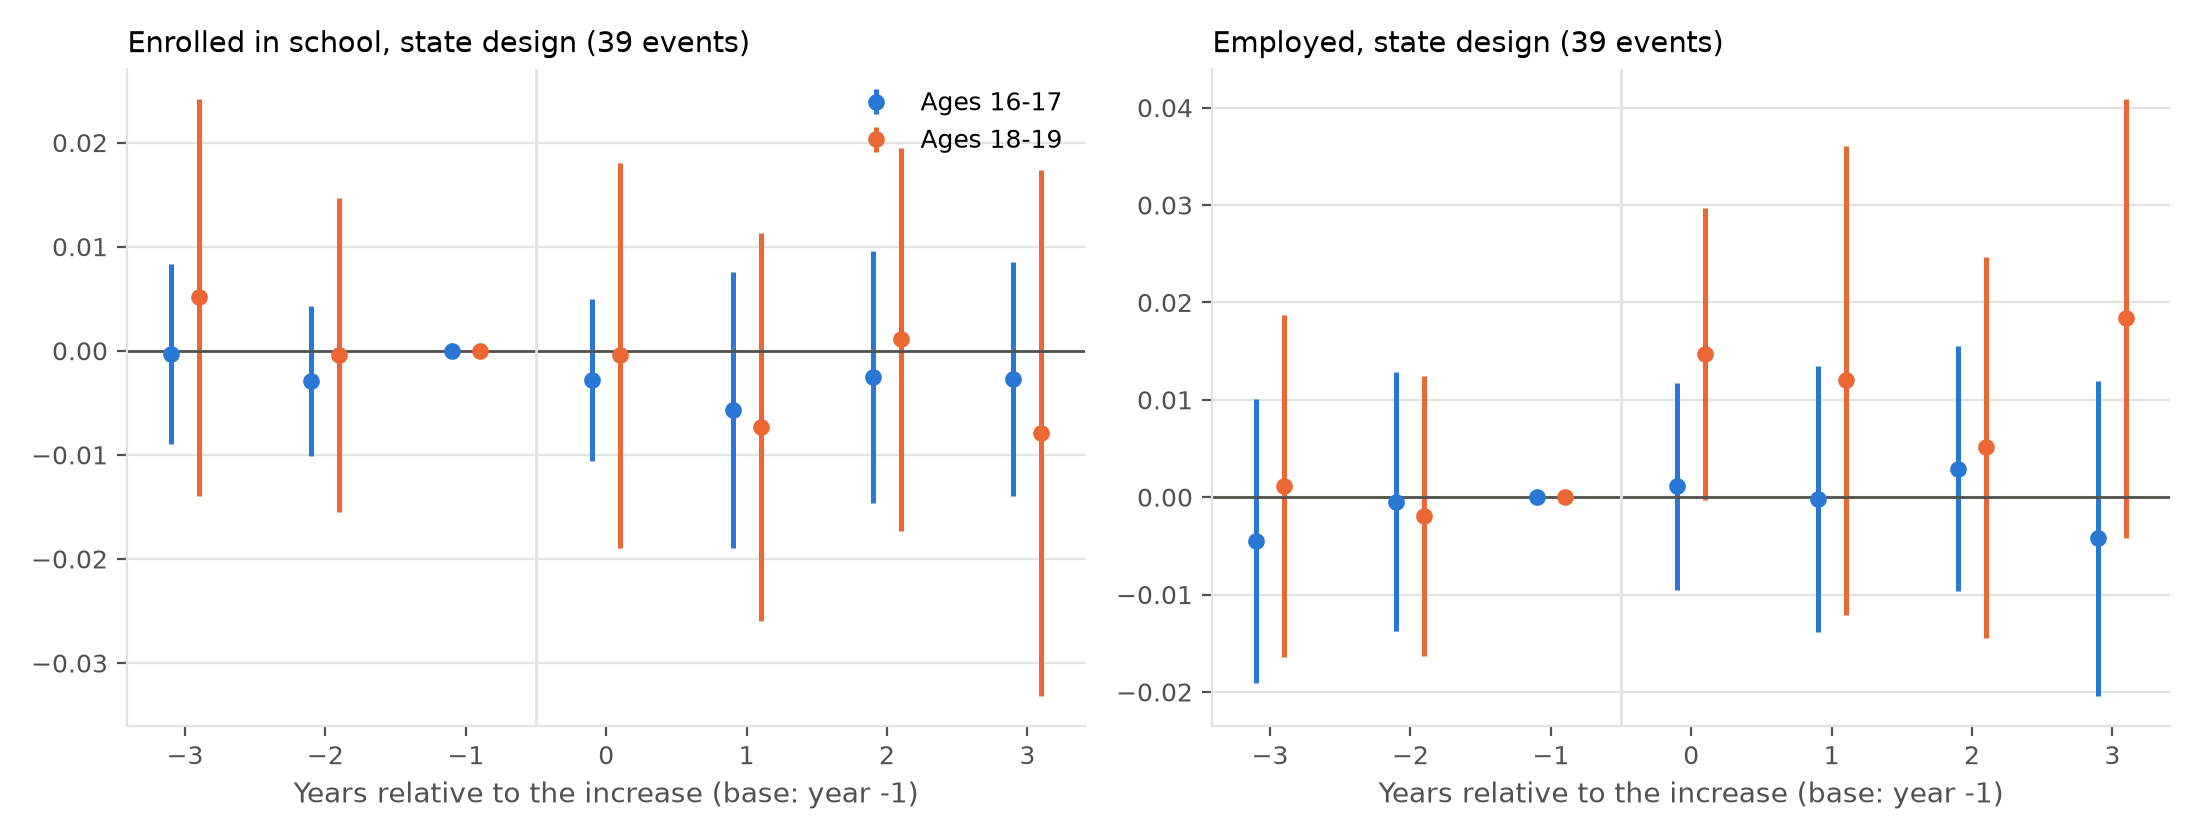
\includegraphics[width=\textwidth]{figures/figA2_state_event_main.png}

\caption{Figure 12: State design: enrollment and employment}

\end{figure}

\begin{figure}
\centering

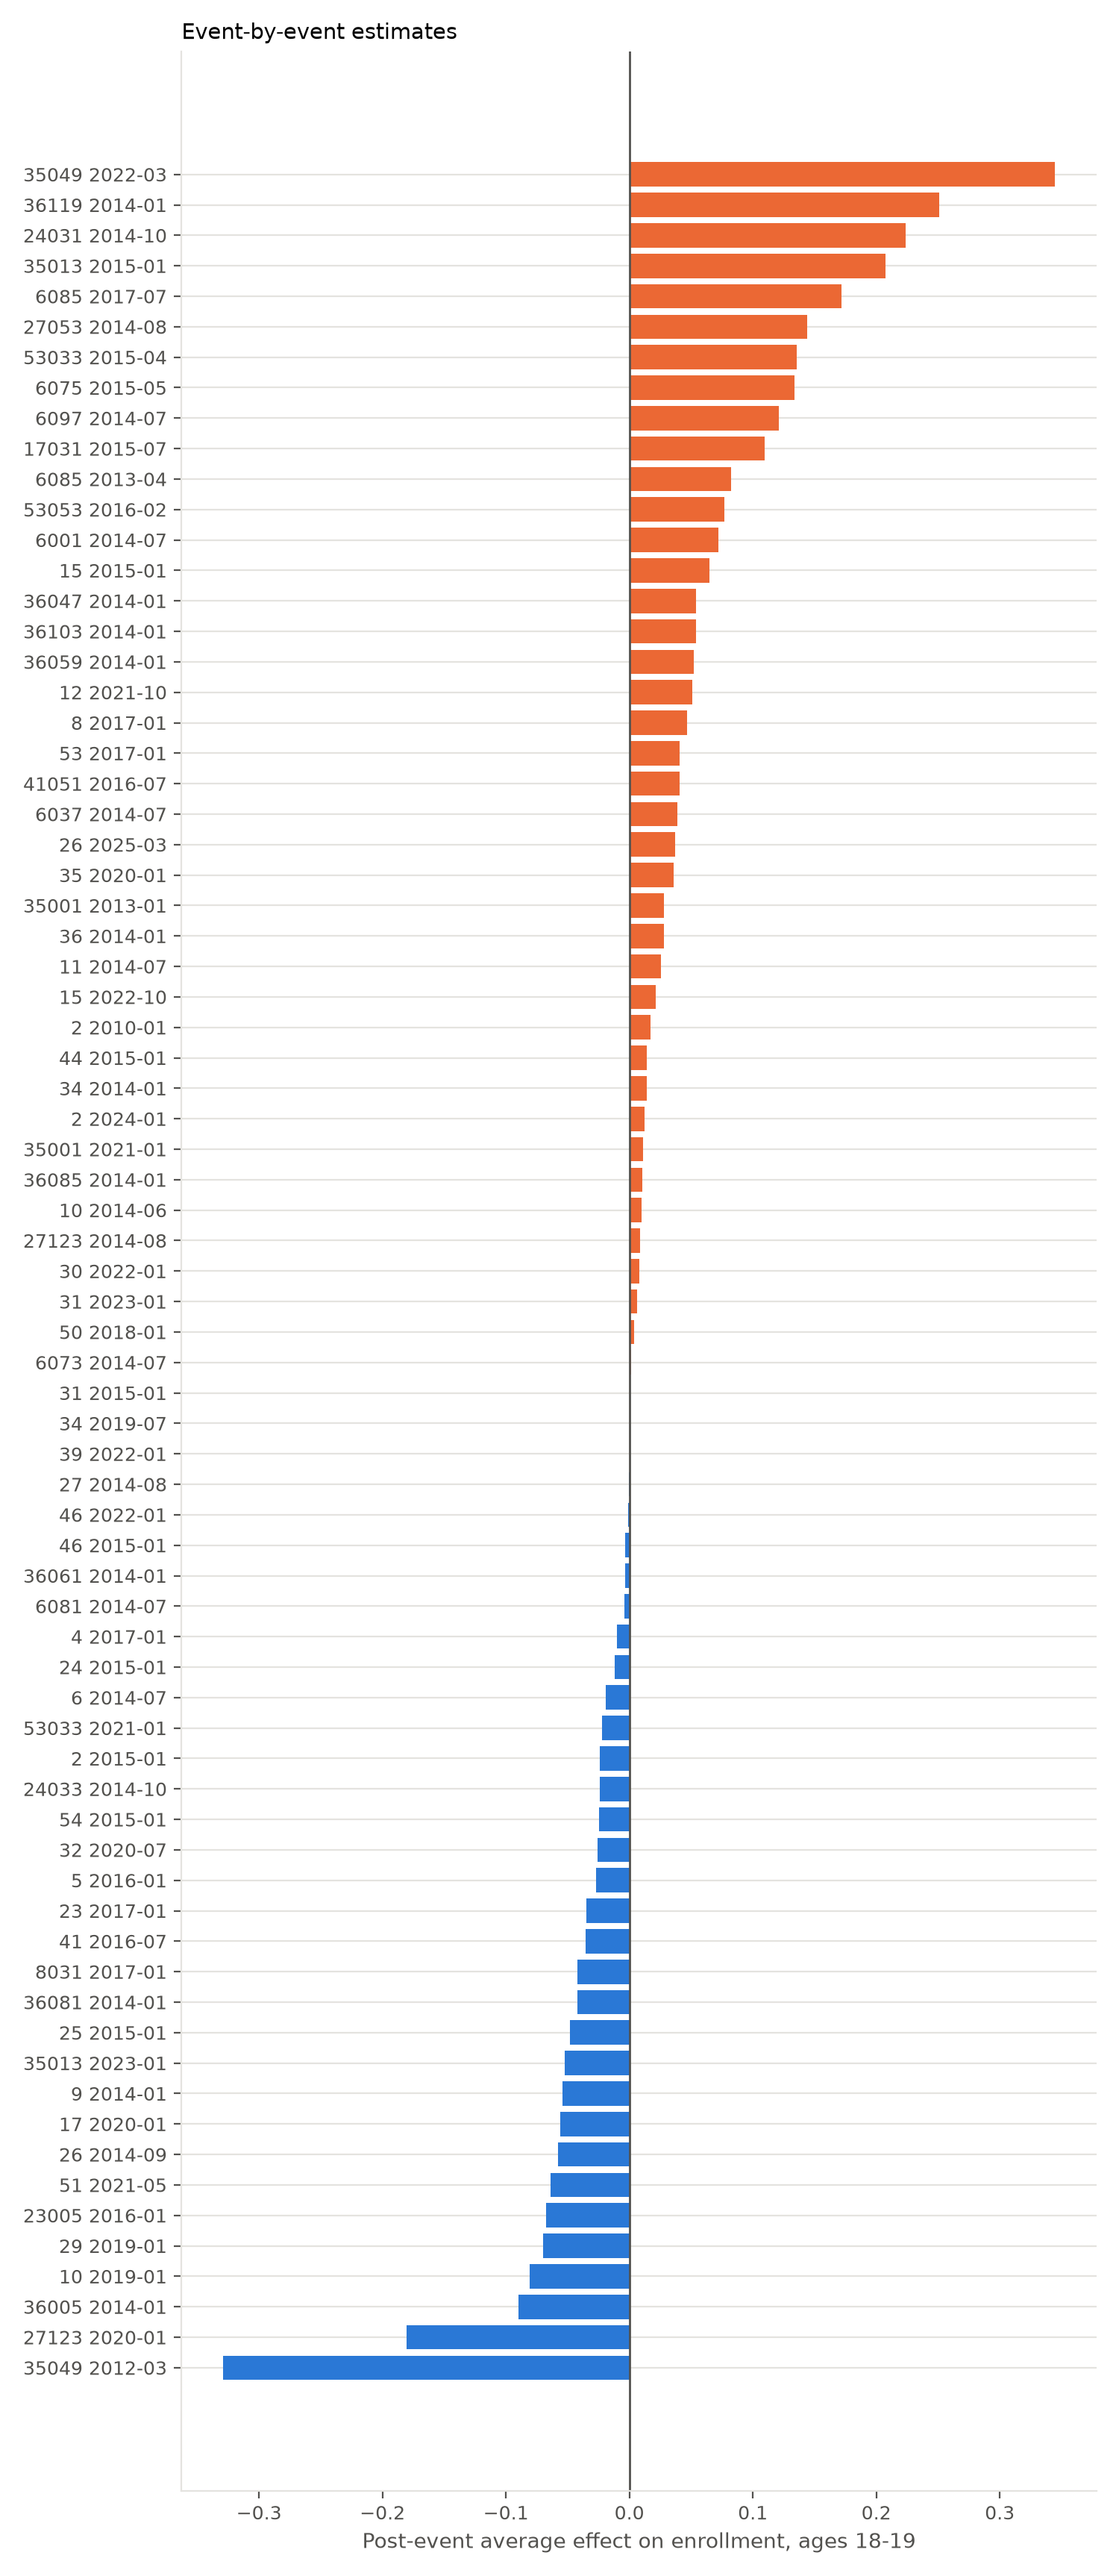
\includegraphics[width=0.85\textwidth]{figures/fig6_byevent.png}

\caption{Figure 13: Event-by-event post-event averages, enrollment of 18--19 year olds}



\noindent\small Notes: Units are state FIPS codes (state remainders) and five-digit county codes (county units); Table 23 names them.
\end{figure}

\section{7 Discussion}

The results match the third case of Section 2. The wage of teens who work rose with the minimum, and by more for teens from poorer families and in the counties with the largest local increases; employment, hours and weekly earnings did not fall; and the allocation of time between school and work did not change for any age, income or racial group; the one movement, among girls aged 16--17, is a shift of about a point from working while in school to school only, with enrollment unchanged, and boys of the same age shift the other way. In a competitive teen labor market a 38 percent rise in the wage floor should have reduced employment or hours, and either the expected wage or the enrollment rate should have moved. Neither did. The pattern is the one a market with employer wage-setting power produces, in which a minimum between the prevailing wage and the marginal product raises pay without reducing the chance of a job, and it is consistent with the bunching estimates of Cengiz et al. (2019) for all low-wage workers and with the direct evidence of concentration in the markets where teens work (Azar et al., 2019; Manning, 2003).

The estimates also rule the minimum wage out as the cause of the decline in teen employment on two counts of timing and one of magnitude. Most of the decline happened before the period studied here, between 2000 and 2010 in the published CPS series, before the large state and local schedules that give the minimum wage its modern bite; within the window, the fall from 36 percent in 2007 to 27 percent in 2010 precedes all but four of the 73 events. The period of the largest increases, 2014--2025, is one in which teen employment rose, from 27 percent in 2010 to 33 percent in 2022. The main estimates imply no contribution at all, and even the most negative cell in Table 13, $-4.7$ points (s.e.\ 5.1) for 18--19 year olds in the 16 local-only county events, applied to every teen in the country, would account for a quarter of the eighteen-point fall, most of which happened before the increases. The decline itself then needs another explanation, and the candidates in Neumark and Shupe (2019) and Smith (2011); Smith (2012) remain: the rising return to schooling and the intensification of college preparation, competition from adult and immigrant workers in the retail and food service jobs that teens held, and the two recessions of the period. This paper's contribution is to remove one from the list.

The absence of a schooling gain for low-income teens does not contradict Smith (2021) so much as bound it for a later period and a different design. His estimate implies that increases of the size studied here would have lowered dropout among low-SES teens by two to four points; the enrollment and dropout intervals for low-income teens here (Appendix E) exclude changes of that size. Two differences could reconcile the findings: his socioeconomic measure is parental education, which identifies a poorer group than family income below the median, and his variation is the smaller increases of 1992--2012 estimated with two-way fixed effects and a distributed-lag specification, which the event design does not reproduce. Appendix C shows what that specification does on the modern data: on all months it finds a small rise in the share of teens neither in school nor at work and a small fall in enrollment at 16--17, for high-income teens as much as for low-income ones; in school months the 16--17 coefficients are a fifth of the size and insignificant, and what remains at 18--19 disappears once the federal-floor states are dropped. The earlier literature's schooling effects, in both directions, are of the size that the choice of months and of comparison states can produce in this specification. What can be said is that in the modern period the poorer half of teens received the wage gain and did not change their schooling in response.

Three limits should be stated. The enrollment measure is attendance last week; it cannot see grade progression or completion, so the null does not rule out effects on attainment measured years later. The 2023--2025 minimum wage changes and index adjustments are compiled from state sources and are less thoroughly vetted than the Vaghul and Zipperer (2016) list; they determine which units are clean controls after 2022 and should be verified before the event list is treated as final. Local minimums are carried at their end-2022 levels thereafter, and a city's rate is applied to its whole county, so a Seattle rate treats all of King County; the county samples are small and the county events are best read alongside the state remainders. Standard errors are from a 99-draw block bootstrap; the wild cluster bootstrap in the Stata replication is the inference to report.

\section{8 Conclusion}

This paper estimates the effect of minimum wage increases on the wages and the time allocation of 16--19 year olds, using the event design the minimum wage employment literature adopted after 2019, with every county that sets its own minimum treated as a jurisdiction of its own, on the 73 large increases since 2010. The increases raised the hourly wages of working teens by 3 to 7 percent, for teens from low- and high-income families alike, and changed nothing else: not the share enrolled and employed, enrolled only, employed only, or neither, at either age or in either income group, and not hours or weekly earnings. The estimates are precise enough to rule out changes larger than a point or two in any share, and they are stable across units, event sets, control groups, weights, the pandemic years and subgroups. A two-period schooling model shows that this is the expected outcome when the wage gain is small relative to the skilled premium and employers set teen wages below the competitive level: the minimum wage raises pay without reducing the probability of a job, and a few hundred dollars a year does not move a decision worth several hundred thousand. The minimum wage is not the culprit in the fall of teen employment, and in the modern period it functioned as a transfer to teenagers who work, with no offsetting cost in their schooling or their jobs.


\bibliographystyle{aer}
\section*{References}

\noindent Acemoglu, Daron. 2009. Lectures in Labor Economics. Lecture notes, Massachusetts Institute of Technology.

\noindent Allegretto, Sylvia, Arindrajit Dube, Michael Reich, and Ben Zipperer. 2017. ``Credible Research Designs for Minimum Wage Studies: A Response to Neumark, Salas, and Wascher.'' \textit{ILR Review} 70 (3): 559--592.

\noindent Azar, Jos\'e, Emiliano Huet-Vaughn, Ioana Marinescu, Bledi Taska, and Till von Wachter. 2019. ``Minimum Wage Employment Effects and Labor Market Concentration.'' NBER Working Paper 26101.

\noindent Baker, Andrew C., David F. Larcker, and Charles C. Y. Wang. 2022. ``How Much Should We Trust Staggered Difference-in-Differences Estimates?'' \textit{Journal of Financial Economics} 144 (2): 370--395.

\noindent Callaway, Brantly, and Pedro H. C. Sant'Anna. 2021. ``Difference-in-Differences with Multiple Time Periods.'' \textit{Journal of Econometrics} 225 (2): 200--230.

\noindent Campolieti, Michele, Tony Fang, and Morley Gunderson. 2005. ``How Minimum Wages Affect Schooling-Employment Outcomes in Canada, 1993--1999.'' \textit{Journal of Labor Research} 26 (3): 533--545.

\noindent Card, David, and Alan B. Krueger. 1994. ``Minimum Wages and Employment: A Case Study of the Fast-Food Industry in New Jersey and Pennsylvania.'' \textit{American Economic Review} 84 (4): 772--793.

\noindent Card, David, and Alan B. Krueger. 1995. \textit{Myth and Measurement: The New Economics of the Minimum Wage}. Princeton: Princeton University Press.

\noindent Cengiz, Doruk, Arindrajit Dube, Attila Lindner, and Ben Zipperer. 2019. ``The Effect of Minimum Wages on Low-Wage Jobs.'' \textit{Quarterly Journal of Economics} 134 (3): 1405--1454.

\noindent Chaplin, Duncan D., Mark D. Turner, and Andreas D. Pape. 2003. ``Minimum Wages and School Enrollment of Teenagers: A Look at the 1990's.'' \textit{Economics of Education Review} 22 (1): 11--21.

\noindent Clemens, Jeffrey, and Michael Wither. 2019. ``The Minimum Wage and the Great Recession: Evidence of Effects on the Employment and Income Trajectories of Low-Skilled Workers.'' \textit{Journal of Public Economics} 170: 53--67.

\noindent de Chaisemartin, Cl\'ement, and Xavier D'Haultf{\oe}uille. 2020. ``Two-Way Fixed Effects Estimators with Heterogeneous Treatment Effects.'' \textit{American Economic Review} 110 (9): 2964--2996.

\noindent de Chaisemartin, Cl\'ement, and Xavier D'Haultf{\oe}uille. 2024. ``Difference-in-Differences Estimators of Intertemporal Treatment Effects.'' \textit{Review of Economics and Statistics}, forthcoming.

\noindent Dube, Arindrajit, T. William Lester, and Michael Reich. 2010. ``Minimum Wage Effects Across State Borders: Estimates Using Contiguous Counties.'' \textit{Review of Economics and Statistics} 92 (4): 945--964.

\noindent Dube, Arindrajit. 2019. ``Impacts of Minimum Wages: Review of the International Evidence.'' Report to the UK Low Pay Commission, HM Treasury.

\noindent Ehrenberg, Ronald G., and Alan J. Marcus. 1982. ``Minimum Wages and Teenagers' Enrollment-Employment Outcomes: A Multinomial Logit Model.'' \textit{Journal of Human Resources} 17 (1): 39--58.

\noindent Flood, Sarah, Miriam King, Renae Rodgers, Steven Ruggles, J. Robert Warren, Daniel Backman, Annie Chen, Grace Cooper, Stephanie Richards, Megan Schouweiler, and Michael Westberry. 2024. \textit{IPUMS CPS: Version 12.0}. Minneapolis, MN: IPUMS.

\noindent Goodman-Bacon, Andrew. 2021. ``Difference-in-Differences with Variation in Treatment Timing.'' \textit{Journal of Econometrics} 225 (2): 254--277.

\noindent Manning, Alan. 2003. \textit{Monopsony in Motion: Imperfect Competition in Labor Markets}. Princeton: Princeton University Press.

\noindent Mincer, Jacob. 1976. ``Unemployment Effects of Minimum Wages.'' \textit{Journal of Political Economy} 84 (4): S87--S104.

\noindent Morisi, Teresa L. 2008. ``Youth Enrollment and Employment during the School Year.'' \textit{Monthly Labor Review} 131 (2): 51--63.

\noindent Meer, Jonathan, and Jeremy West. 2016. ``Effects of the Minimum Wage on Employment Dynamics.'' \textit{Journal of Human Resources} 51 (2): 500--522.

\noindent Neumark, David, and Cortnie Shupe. 2019. ``Declining Teen Employment: Minimum Wages, Returns to Schooling, and Immigration.'' \textit{Labour Economics} 59: 49--68.

\noindent Neumark, David, and William Wascher. 1995a. ``Minimum Wage Effects on Employment and School Enrollment.'' \textit{Journal of Business and Economic Statistics} 13 (2): 199--206.

\noindent Neumark, David, and William Wascher. 1995b. ``Minimum-Wage Effects on School and Work Transitions of Teenagers.'' \textit{American Economic Review} 85 (2): 244--249.

\noindent Neumark, David, and William Wascher. 2003. ``Minimum Wages and Skill Acquisition: Another Look at Schooling Effects.'' \textit{Economics of Education Review} 22 (1): 1--10.

\noindent Robinson, Joan. 1933. \textit{The Economics of Imperfect Competition}. London: Macmillan.

\noindent Smith, Christopher L. 2011. ``Polarization, Immigration, Education: What's Behind the Dramatic Decline in Youth Employment?'' Finance and Economics Discussion Series 2011-41, Federal Reserve Board.

\noindent Smith, Christopher L. 2012. ``The Impact of Low-Skilled Immigration on the Youth Labor Market.'' \textit{Journal of Labor Economics} 30 (1): 55--89.

\noindent Smith, Alexander A. 2021. ``The Minimum Wage and Teen Educational Attainment.'' \textit{Labour Economics} 73: 102061.

\noindent Stigler, George J. 1946. ``The Economics of Minimum Wage Legislation.'' \textit{American Economic Review} 36 (3): 358--365.

\noindent Sun, Liyang, and Sarah Abraham. 2021. ``Estimating Dynamic Treatment Effects in Event Studies with Heterogeneous Treatment Effects.'' \textit{Journal of Econometrics} 225 (2): 175--199.

\noindent Vaghul, Kavya, and Ben Zipperer. 2016. ``Historical State and Sub-State Minimum Wage Data.'' Washington Center for Equitable Growth Working Paper.

\noindent Warren, John Robert, and Caitlin Hamrock. 2010. ``The Effect of Minimum Wage Rates on High School Completion.'' \textit{Social Forces} 88 (3): 1379--1392.




\appendix
\section{A Post-event average tables}

Tables 15 to 18 collect the post-event averages that Section 5 discusses. Each reports the post-event average effect of the increases, the mean of the relative-year effects for the four years from the increase relative to the year before it, population-weighted across the 73 events from 2010, with the block-bootstrap standard error beneath and the average of the two pre-event coefficients beside it. Table 15 gives the four school--work shares, enrollment and employment for all teens by age; Tables 16 and 17 repeat it for teens from families with income below \$50,000 and at or above it; Table 18 gives the log hourly wage of hourly-paid teens and the log weekly earnings of all teen workers; Tables 19 to 22 repeat Table 15 for girls, boys, non-Hispanic white teens and all other teens.

\begin{table}
\centering
\caption{Table 15: Effects of minimum wage increases on teen school--work status: post-event averages, 73 events from 2010}

\small
\begin{tabular}{p{0.30\textwidth}p{0.113\textwidth}p{0.113\textwidth}p{0.113\textwidth}p{0.113\textwidth}p{0.113\textwidth}p{0.113\textwidth}}
\toprule
 & \multicolumn{2}{c}{Ages 16--17} & \multicolumn{2}{c}{Ages 18--19} & \multicolumn{2}{c}{Ages 16--19} \\

 & Post & Pre & Post & Pre & Post & Pre \\
\midrule
Enrolled and employed & -0.003 & -0.002 & 0.007 & 0.002 & 0.001 & -0.001 \\
 & (0.005) &  & (0.006) &  & (0.004) &  \\
Enrolled only & -0.000 & 0.001 & -0.005 & 0.003 & -0.001 & 0.006 \\
 & (0.006) &  & (0.006) &  & (0.003) &  \\
Employed only & 0.002 & -0.002 & 0.003 & -0.005 & 0.002 & -0.005 \\
 & (0.003) &  & (0.007) &  & (0.004) &  \\
Neither enrolled nor employed & 0.001 & 0.003 & -0.005 & -0.001 & -0.002 & -0.000 \\
 & (0.004) &  & (0.005) &  & (0.003) &  \\
Enrolled (first two rows) & -0.003 & -0.001 & 0.001 & 0.006 & 0.001 & 0.005 \\
 & (0.004) &  & (0.009) &  & (0.005) &  \\
Employed (first and third rows) & -0.001 & -0.003 & 0.010 & -0.002 & 0.003 & -0.006 \\
 & (0.005) &  & (0.007) &  & (0.004) &  \\
\bottomrule
\end{tabular}



\noindent\small Notes: Post: average of the relative-year effects for years 0--3 after the increase, relative to year $-1$, population-weighted across events; block-bootstrap standard errors over states in parentheses (99 draws). Pre: average of the relative-year effects for years $-3$ and $-2$. \textsuperscript{*}, \textsuperscript{**}, \textsuperscript{***}: significant at 10, 5 and 1 percent.

\end{table}

\begin{table}
\centering
\caption{Table 16: Effects on school--work status, teens from families with income below \$50,000: post-event averages}

\small
\begin{tabular}{p{0.30\textwidth}p{0.113\textwidth}p{0.113\textwidth}p{0.113\textwidth}p{0.113\textwidth}p{0.113\textwidth}p{0.113\textwidth}}
\toprule
 & \multicolumn{2}{c}{Ages 16--17} & \multicolumn{2}{c}{Ages 18--19} & \multicolumn{2}{c}{Ages 16--19} \\

 & Post & Pre & Post & Pre & Post & Pre \\
\midrule
Enrolled and employed & 0.004 & 0.005 & 0.006 & 0.008 & 0.005 & 0.006 \\
 & (0.008) &  & (0.007) &  & (0.005) &  \\
Enrolled only & -0.005 & -0.007 & -0.002 & -0.003 & -0.005 & -0.006 \\
 & (0.010) &  & (0.009) &  & (0.007) &  \\
Employed only & -0.002 & -0.003 & 0.006 & -0.001 & 0.003 & -0.002 \\
 & (0.004) &  & (0.011) &  & (0.006) &  \\
Neither enrolled nor employed & 0.003 & 0.005 & -0.010 & -0.004 & -0.003 & 0.001 \\
 & (0.005) &  & (0.007) &  & (0.005) &  \\
Enrolled (first two rows) & -0.001 & -0.001 & 0.004 & 0.005 & 0.000 & 0.001 \\
 & (0.006) &  & (0.012) &  & (0.006) &  \\
Employed (first and third rows) & 0.002 & 0.002 & 0.012 & 0.007 & 0.007 & 0.005 \\
 & (0.010) &  & (0.011) &  & (0.008) &  \\
\bottomrule
\end{tabular}



\noindent\small Notes: Family income is the CPS household income category, nominal; teens with missing or refused income (7 percent) are excluded. Post, Pre and standard errors as in Table 15.

\end{table}

\begin{table}
\centering
\caption{Table 17: Effects on school--work status, teens from families with income of \$50,000 or more: post-event averages}

\small
\begin{tabular}{p{0.30\textwidth}p{0.113\textwidth}p{0.113\textwidth}p{0.113\textwidth}p{0.113\textwidth}p{0.113\textwidth}p{0.113\textwidth}}
\toprule
 & \multicolumn{2}{c}{Ages 16--17} & \multicolumn{2}{c}{Ages 18--19} & \multicolumn{2}{c}{Ages 16--19} \\

 & Post & Pre & Post & Pre & Post & Pre \\
\midrule
Enrolled and employed & -0.006 & -0.008 & 0.009 & -0.001 & 0.000 & -0.006 \\
 & (0.005) &  & (0.009) &  & (0.005) &  \\
Enrolled only & 0.002 & 0.007 & -0.006 & 0.007 & 0.002 & 0.013 \\
 & (0.006) &  & (0.008) &  & (0.004) &  \\
Employed only & 0.005 & -0.001 & 0.003 & -0.006 & 0.002 & -0.007 \\
 & (0.003) &  & (0.009) &  & (0.005) &  \\
Neither enrolled nor employed & -0.001 & 0.001 & -0.005 & -0.001 & -0.003 & -0.001 \\
 & (0.004) &  & (0.006) &  & (0.004) &  \\
Enrolled (first two rows) & -0.004 & -0.000 & 0.002 & 0.006 & 0.002 & 0.007 \\
 & (0.005) &  & (0.012) &  & (0.006) &  \\
Employed (first and third rows) & -0.001 & -0.009 & 0.011 & -0.006 & 0.002 & -0.012 \\
 & (0.005) &  & (0.008) &  & (0.004) &  \\
\bottomrule
\end{tabular}



\noindent\small Notes: Family income is the CPS household income category, nominal; teens with missing or refused income (7 percent) are excluded. Post, Pre and standard errors as in Table 15.

\end{table}

\begin{table}
\centering
\caption{Table 18: Effects of minimum wage increases on teen wages and earnings: post-event averages, 73 events from 2010}

\small
\begin{tabular}{p{0.30\textwidth}p{0.113\textwidth}p{0.113\textwidth}p{0.113\textwidth}p{0.113\textwidth}p{0.113\textwidth}p{0.113\textwidth}}
\toprule
 & \multicolumn{2}{c}{Ages 16--17} & \multicolumn{2}{c}{Ages 18--19} & \multicolumn{2}{c}{Ages 16--19} \\

 & Post & Pre & Post & Pre & Post & Pre \\
\midrule
Log hourly wage, hourly-paid teens & 0.053\textsuperscript{***} & -0.005 & 0.030\textsuperscript{***} & -0.000 & 0.038\textsuperscript{***} & -0.003 \\
 & (0.012) &  & (0.008) &  & (0.009) &  \\
Log weekly earnings, all teen workers & 0.049 & -0.007 & 0.042\textsuperscript{*} & 0.005 & 0.046\textsuperscript{*} & -0.002 \\
 & (0.032) &  & (0.024) &  & (0.024) &  \\
\bottomrule
\end{tabular}



\noindent\small Notes: Outgoing rotation groups, earnings weights. Hourly wage among workers paid by the hour; weekly earnings among all workers. Block-bootstrap standard errors in parentheses.

\end{table}

\begin{table}
\centering
\caption{Table 19: Effects on school--work status, girls: post-event averages}

\small
\begin{tabular}{p{0.30\textwidth}p{0.113\textwidth}p{0.113\textwidth}p{0.113\textwidth}p{0.113\textwidth}p{0.113\textwidth}p{0.113\textwidth}}
\toprule
 & \multicolumn{2}{c}{Ages 16--17} & \multicolumn{2}{c}{Ages 18--19} & \multicolumn{2}{c}{Ages 16--19} \\

 & Post & Pre & Post & Pre & Post & Pre \\
\midrule
Enrolled and employed & -0.013\textsuperscript{***} & 0.000 & 0.008 & 0.014 & -0.003 & 0.005 \\
 & (0.005) &  & (0.010) &  & (0.005) &  \\
Enrolled only & 0.012\textsuperscript{*} & 0.001 & 0.005 & 0.018 & 0.012\textsuperscript{*} & 0.016 \\
 & (0.007) &  & (0.009) &  & (0.007) &  \\
Employed only & -0.000 & -0.000 & -0.002 & -0.018 & -0.003 & -0.012 \\
 & (0.003) &  & (0.009) &  & (0.005) &  \\
Neither enrolled nor employed & 0.001 & -0.002 & -0.011 & -0.014 & -0.005 & -0.009 \\
 & (0.005) &  & (0.008) &  & (0.005) &  \\
Enrolled (first two rows) & -0.001 & 0.002 & 0.013 & 0.032 & 0.008 & 0.020 \\
 & (0.005) &  & (0.011) &  & (0.007) &  \\
Employed (first and third rows) & -0.013\textsuperscript{***} & 0.000 & 0.007 & -0.004 & -0.006 & -0.007 \\
 & (0.005) &  & (0.011) &  & (0.006) &  \\
\bottomrule
\end{tabular}



\noindent\small Notes: Post, Pre and standard errors as in Table 15.

\end{table}

\begin{table}
\centering
\caption{Table 20: Effects on school--work status, boys: post-event averages}

\small
\begin{tabular}{p{0.30\textwidth}p{0.113\textwidth}p{0.113\textwidth}p{0.113\textwidth}p{0.113\textwidth}p{0.113\textwidth}p{0.113\textwidth}}
\toprule
 & \multicolumn{2}{c}{Ages 16--17} & \multicolumn{2}{c}{Ages 18--19} & \multicolumn{2}{c}{Ages 16--19} \\

 & Post & Pre & Post & Pre & Post & Pre \\
\midrule
Enrolled and employed & 0.008 & -0.005 & 0.005 & -0.007 & 0.006 & -0.006 \\
 & (0.010) &  & (0.007) &  & (0.007) &  \\
Enrolled only & -0.012 & 0.001 & -0.016\textsuperscript{*} & -0.014 & -0.014\textsuperscript{***} & -0.005 \\
 & (0.010) &  & (0.009) &  & (0.005) &  \\
Employed only & 0.004 & -0.003 & 0.009 & 0.009 & 0.006 & 0.003 \\
 & (0.005) &  & (0.009) &  & (0.005) &  \\
Neither enrolled nor employed & 0.000 & 0.007 & 0.001 & 0.011 & 0.001 & 0.008 \\
 & (0.004) &  & (0.006) &  & (0.003) &  \\
Enrolled (first two rows) & -0.004 & -0.004 & -0.011 & -0.020 & -0.007 & -0.011 \\
 & (0.006) &  & (0.010) &  & (0.005) &  \\
Employed (first and third rows) & 0.012 & -0.008 & 0.015 & 0.003 & 0.013\textsuperscript{**} & -0.004 \\
 & (0.009) &  & (0.009) &  & (0.006) &  \\
\bottomrule
\end{tabular}



\noindent\small Notes: Post, Pre and standard errors as in Table 15.

\end{table}

\begin{table}
\centering
\caption{Table 21: Effects on school--work status, non-Hispanic white teens: post-event averages}

\small
\begin{tabular}{p{0.30\textwidth}p{0.113\textwidth}p{0.113\textwidth}p{0.113\textwidth}p{0.113\textwidth}p{0.113\textwidth}p{0.113\textwidth}}
\toprule
 & \multicolumn{2}{c}{Ages 16--17} & \multicolumn{2}{c}{Ages 18--19} & \multicolumn{2}{c}{Ages 16--19} \\

 & Post & Pre & Post & Pre & Post & Pre \\
\midrule
Enrolled and employed & 0.003 & -0.000 & 0.000 & 0.013 & 0.002 & 0.005 \\
 & (0.007) &  & (0.010) &  & (0.006) &  \\
Enrolled only & -0.002 & 0.004 & -0.009 & -0.005 & -0.004 & 0.002 \\
 & (0.007) &  & (0.008) &  & (0.006) &  \\
Employed only & 0.002 & -0.001 & 0.006 & -0.009 & 0.003 & -0.007 \\
 & (0.004) &  & (0.010) &  & (0.006) &  \\
Neither enrolled nor employed & -0.003 & -0.003 & 0.003 & 0.001 & -0.001 & -0.001 \\
 & (0.005) &  & (0.007) &  & (0.005) &  \\
Enrolled (first two rows) & 0.000 & 0.004 & -0.009 & 0.007 & -0.002 & 0.008 \\
 & (0.007) &  & (0.012) &  & (0.008) &  \\
Employed (first and third rows) & 0.005 & -0.001 & 0.006 & 0.004 & 0.004 & -0.001 \\
 & (0.007) &  & (0.010) &  & (0.007) &  \\
\bottomrule
\end{tabular}



\noindent\small Notes: Post, Pre and standard errors as in Table 15.

\end{table}

\begin{table}
\centering
\caption{Table 22: Effects on school--work status, Black, Hispanic and other non-white teens: post-event averages}

\small
\begin{tabular}{p{0.30\textwidth}p{0.113\textwidth}p{0.113\textwidth}p{0.113\textwidth}p{0.113\textwidth}p{0.113\textwidth}p{0.113\textwidth}}
\toprule
 & \multicolumn{2}{c}{Ages 16--17} & \multicolumn{2}{c}{Ages 18--19} & \multicolumn{2}{c}{Ages 16--19} \\

 & Post & Pre & Post & Pre & Post & Pre \\
\midrule
Enrolled and employed & -0.012\textsuperscript{*} & -0.003 & 0.011 & -0.007 & -0.001 & -0.006 \\
 & (0.007) &  & (0.007) &  & (0.005) &  \\
Enrolled only & 0.007 & -0.001 & 0.002 & 0.009 & 0.005 & 0.007 \\
 & (0.012) &  & (0.011) &  & (0.008) &  \\
Employed only & 0.001 & -0.003 & -0.000 & 0.003 & -0.001 & -0.002 \\
 & (0.004) &  & (0.010) &  & (0.005) &  \\
Neither enrolled nor employed & 0.003 & 0.007 & -0.012 & -0.006 & -0.004 & 0.000 \\
 & (0.005) &  & (0.008) &  & (0.005) &  \\
Enrolled (first two rows) & -0.004 & -0.004 & 0.012 & 0.003 & 0.004 & 0.001 \\
 & (0.007) &  & (0.010) &  & (0.006) &  \\
Employed (first and third rows) & -0.011 & -0.007 & 0.010 & -0.003 & -0.001 & -0.008 \\
 & (0.009) &  & (0.013) &  & (0.009) &  \\
\bottomrule
\end{tabular}



\noindent\small Notes: Post, Pre and standard errors as in Table 15.

\end{table}


\section{B The events}

\begin{table}
\centering
\caption{Table 23: Unit events from January 2010 with CPS teens in the unit}

\scriptsize
\begin{tabular}{lllrrrrrr}
\toprule
Unit & Source & Event month & Before & First step & End of window & Rise (\%) & Steps & Controls \\
\midrule
Alaska (remainder) & state & 2010-01 & 7.25 & 7.75 & 7.75 & 7 & 1 & 26 \\
Connecticut (remainder) & state & 2014-01 & 8.25 & 8.70 & 10.10 & 22 & 3 & 29 \\
New Jersey (remainder) & state & 2014-01 & 7.25 & 8.25 & 8.44 & 16 & 1 & 29 \\
New York (remainder) & state & 2014-01 & 7.25 & 8.00 & 9.70 & 34 & 3 & 29 \\
Delaware (remainder) & state & 2014-06 & 7.25 & 7.75 & 8.25 & 14 & 2 & 28 \\
California (remainder) & state & 2014-07 & 8.00 & 9.00 & 11.00 & 38 & 3 & 28 \\
District of Columbia (remainder) & state & 2014-07 & 8.25 & 9.50 & 12.50 & 52 & 4 & 28 \\
Minnesota (remainder) & state & 2014-08 & 7.25 & 8.00 & 9.65 & 33 & 3 & 28 \\
Michigan (remainder) & state & 2014-09 & 7.40 & 8.15 & 9.25 & 25 & 1 & 28 \\
Alaska (remainder) & state & 2015-01 & 7.75 & 8.75 & 9.84 & 27 & 2 & 28 \\
Hawaii (remainder) & state & 2015-01 & 7.25 & 7.75 & 10.10 & 39 & 4 & 28 \\
Maryland (remainder) & state & 2015-01 & 7.25 & 8.00 & 10.10 & 39 & 4 & 28 \\
Massachusetts (remainder) & state & 2015-01 & 8.00 & 9.00 & 11.00 & 38 & 3 & 28 \\
Nebraska (remainder) & state & 2015-01 & 7.25 & 8.00 & 9.00 & 24 & 2 & 28 \\
Rhode Island (remainder) & state & 2015-01 & 8.00 & 9.00 & 10.10 & 26 & 3 & 28 \\
South Dakota (remainder) & state & 2015-01 & 7.25 & 8.50 & 8.85 & 22 & 1 & 28 \\
West Virginia (remainder) & state & 2015-01 & 7.25 & 8.00 & 8.75 & 21 & 2 & 28 \\
Arkansas (remainder) & state & 2016-01 & 7.50 & 8.00 & 9.25 & 23 & 3 & 28 \\
Oregon (remainder) & state & 2016-07 & 9.25 & 9.75 & 11.25 & 22 & 2 & 27 \\
Arizona (remainder) & state & 2017-01 & 8.05 & 10.00 & 12.00 & 49 & 3 & 26 \\
Colorado (remainder) & state & 2017-01 & 8.31 & 9.30 & 12.00 & 44 & 4 & 26 \\
Maine (remainder) & state & 2017-01 & 7.50 & 9.00 & 12.00 & 60 & 4 & 26 \\
Washington (remainder) & state & 2017-01 & 9.47 & 11.00 & 13.50 & 43 & 2 & 26 \\
Vermont (remainder) & state & 2018-01 & 10.00 & 10.50 & 11.75 & 18 & 2 & 24 \\
Delaware (remainder) & state & 2019-01 & 8.25 & 8.75 & 10.50 & 27 & 3 & 22 \\
Missouri (remainder) & state & 2019-01 & 7.85 & 8.60 & 11.15 & 42 & 4 & 22 \\
New Jersey (remainder) & state & 2019-07 & 8.85 & 10.00 & 14.00 & 58 & 5 & 24 \\
Illinois (remainder) & state & 2020-01 & 8.25 & 9.25 & 13.00 & 58 & 5 & 27 \\
New Mexico (remainder) & state & 2020-01 & 7.50 & 9.00 & 12.00 & 60 & 3 & 27 \\
Nevada (remainder) & state & 2020-07 & 8.25 & 9.00 & 11.25 & 36 & 4 & 29 \\
Virginia (remainder) & state & 2021-05 & 7.25 & 9.50 & 13.50 & 86 & 4 & 30 \\
Florida (remainder) & state & 2021-10 & 8.56 & 10.00 & 13.00 & 52 & 4 & 49 \\
Montana (remainder) & state & 2022-01 & 8.75 & 9.20 & 10.55 & 21 & 2 & 49 \\
Ohio (remainder) & state & 2022-01 & 8.80 & 9.30 & 10.70 & 22 & 2 & 49 \\
South Dakota (remainder) & state & 2022-01 & 9.45 & 9.95 & 11.50 & 22 & 2 & 49 \\
Hawaii (remainder) & state & 2022-10 & 10.10 & 12.00 & 14.00 & 39 & 2 & 57 \\
Nebraska (remainder) & state & 2023-01 & 9.00 & 10.50 & 13.50 & 50 & 3 & 57 \\
Alaska (remainder) & state & 2024-01 & 10.85 & 11.73 & 13.00 & 20 & 2 & 59 \\
Michigan (remainder) & state & 2025-03 & 10.56 & 12.48 & 12.48 & 18 & 1 & 73 \\
Santa Fe (New Mexico) & local & 2012-03 & 9.50 & 10.29 & 10.84 & 14 & 1 & 54 \\
Bernalillo (Albuquerque) (New Mexico) & local & 2013-01 & 7.50 & 8.50 & 8.75 & 17 & 1 & 53 \\
Santa Clara (California) & local & 2013-04 & 8.00 & 10.00 & 10.50 & 31 & 1 & 46 \\
Bronx (New York) & both & 2014-01 & 7.25 & 8.00 & 11.00 & 52 & 3 & 29 \\
Kings (Brooklyn) (New York) & both & 2014-01 & 7.25 & 8.00 & 11.00 & 52 & 3 & 29 \\
Nassau (New York) & both & 2014-01 & 7.25 & 8.00 & 10.00 & 38 & 3 & 29 \\
New York (Manhattan) (New York) & both & 2014-01 & 7.25 & 8.00 & 11.00 & 52 & 3 & 29 \\
Queens (New York) & both & 2014-01 & 7.25 & 8.00 & 11.00 & 52 & 3 & 29 \\
Richmond (Staten Island) (New York) & both & 2014-01 & 7.25 & 8.00 & 11.00 & 52 & 3 & 29 \\
Suffolk (New York) & both & 2014-01 & 7.25 & 8.00 & 10.00 & 38 & 3 & 29 \\
Westchester (New York) & both & 2014-01 & 7.25 & 8.00 & 10.00 & 38 & 3 & 29 \\
Alameda (California) & both & 2014-07 & 8.00 & 9.00 & 13.23 & 65 & 2 & 28 \\
Los Angeles (California) & both & 2014-07 & 8.00 & 9.00 & 12.00 & 50 & 4 & 28 \\
San Diego (California) & both & 2014-07 & 8.00 & 9.00 & 11.50 & 44 & 4 & 28 \\
San Mateo (California) & both & 2014-07 & 8.00 & 9.00 & 13.50 & 69 & 4 & 28 \\
Sonoma (California) & both & 2014-07 & 8.00 & 9.00 & 11.00 & 38 & 3 & 28 \\
Hennepin (Minneapolis) (Minnesota) & both & 2014-08 & 7.25 & 8.00 & 11.25 & 55 & 5 & 28 \\
Ramsey (St. Paul) (Minnesota) & both & 2014-08 & 7.25 & 8.00 & 9.65 & 33 & 3 & 28 \\
Montgomery MD (Maryland) & local & 2014-10 & 7.25 & 8.40 & 12.25 & 69 & 5 & 28 \\
Prince George's (Maryland) & local & 2014-10 & 7.25 & 8.40 & 11.50 & 59 & 4 & 28 \\
Dona Ana (Las Cruces) (New Mexico) & local & 2015-01 & 7.50 & 8.40 & 9.20 & 23 & 2 & 27 \\
King (Seattle) (Washington) & local & 2015-04 & 9.47 & 11.00 & 16.00 & 69 & 3 & 28 \\
San Francisco (California) & local & 2015-05 & 11.05 & 12.25 & 15.00 & 36 & 4 & 28 \\
Cook (Chicago) (Illinois) & local & 2015-07 & 8.25 & 10.00 & 12.00 & 45 & 3 & 27 \\
Cumberland (Portland ME) (Maine) & local & 2016-01 & 7.50 & 10.10 & 11.00 & 47 & 2 & 28 \\
Pierce (Tacoma) (Washington) & local & 2016-02 & 9.47 & 10.35 & 12.35 & 30 & 3 & 27 \\
Multnomah (Portland) (Oregon) & both & 2016-07 & 9.25 & 9.75 & 12.50 & 35 & 3 & 27 \\
Denver (Colorado) & both & 2017-01 & 8.31 & 9.30 & 12.85 & 55 & 4 & 26 \\
Santa Clara (California) & local & 2017-07 & 10.50 & 12.00 & 15.45 & 47 & 3 & 24 \\
Ramsey (St. Paul) (Minnesota) & local & 2020-01 & 9.86 & 12.50 & 15.00 & 52 & 2 & 26 \\
Bernalillo (Albuquerque) (New Mexico) & both & 2021-01 & 9.35 & 10.50 & 11.50 & 23 & 2 & 30 \\
King (Seattle) (Washington) & local & 2021-01 & 15.75 & 16.69 & 17.27 & 10 & 1 & 30 \\
Santa Fe (New Mexico) & local & 2022-03 & 12.32 & 12.95 & 12.95 & 5 & 1 & 57 \\
Dona Ana (Las Cruces) (New Mexico) & local & 2023-01 & 10.50 & 11.50 & 11.50 & 10 & 1 & 57 \\
\bottomrule
\end{tabular}



\noindent\small Notes: Units: state remainders (the state outside its counties with a local minimum) and counties with their own minimum. Source: whether the rise came from the state rate, the local rate, or both in the same month. Before: effective minimum in the month before the event. First step: minimum in the event month. End of window: minimum 47 months after the event. Rise: end of window relative to before. Steps: number of increases of 5 percent or more in the window. Controls: units in other states with no increase of 5 percent or more from 36 months before to 47 months after the event. County rates are the county-wide rate where one exists and otherwise the largest city's, applied to the whole county. Alaska 2024 and Michigan 2025 rest on the post-2022 additions to the change list. Source: Vaghul and Zipperer (2016), extended by the author.

\end{table}


\section{C Two-way fixed effects estimates}

This appendix reports the two-way fixed effects regression of the earlier literature, the specification of Neumark and Shupe (2019) and, with lags added, of Smith (2021):
\begin{equation}
y_{it} = \beta \ln MW_{u(i),t} + X_i'\gamma + \alpha_{u(i)} + \lambda_t + \varepsilon_{it},

\end{equation}
estimated on every teen observed from January 2010 with unit and year-month fixed effects, controls for single year of age, sex, race and Hispanic origin, survey weights, and standard errors clustered by state. $\beta$ is the effect of a 100 log-point rise in the effective minimum of the teen's unit; multiplied by 0.32, the log of the average event's 38 percent cumulative rise, it is on the scale of the post-event averages in the text. The regression uses all within-unit variation in the log minimum over sixteen years, the small annual steps and indexation as well as the large increases, and compares units at every point of their schedules with one another and with the federal-floor states, so it carries the weighting problems of Goodman-Bacon (2021) and loads any long-run divergence between raising and non-raising units onto the minimum wage.

Tables 24 to 27 report the coefficients for the outcomes of Section 5, estimated on school months, September to May. The restriction matters for the enrollment outcomes and not for the wage. The CPS enrollment item asks whether the respondent attended school last week, and in June to August it records summer school: 63 percent of 16--17 year olds report enrollment in summer against 93 percent in school months, and the neither share is 25 percent in summer against 4 percent. On all months the coefficient for neither enrolled nor employed is 0.022 (s.e.\ 0.007) at 16--17 and the coefficient for enrollment $-0.021$ (0.010), the signs and magnitudes of the two-way fixed effects literature (Neumark and Wascher, 1995a; Neumark and Shupe, 2019); in June to August alone they are 0.067 (0.017) and $-0.067$ (0.029), and in school months 0.006 (0.008) and $-0.006$ (0.010), a fifth of their all-months size and within one standard error of zero. The all-months regression measures summer school attendance, which is lower where the minimum is higher, not the schooling decision this paper and Smith (2021) are about, and the tables therefore report school months.

In school months the school--work coefficients are small and, with one exception, insignificant: enrolled-and-employed changes by $-0.022$ (0.016) at 16--17 for a 100 log-point rise, $-0.7$ points for the average event, and neither by 0.006 (0.008). The exception is neither at 18--19, 0.017 (0.006), and pooled, 0.012 (0.003). Table 32 shows that it rests on the comparison of the raising units with the federal-floor states: among units whose minimum changed at all between 2010 and 2026, so that identification comes from the timing of increases rather than from sixteen years of divergence between two blocks of states, the school-months coefficient is $-0.005$ (0.017) at 18--19 and 0.008 (0.010) pooled. By family income (Table 25) the neither coefficient at 16--17 is 0.005 (0.011) for low-income and 0.006 (0.008) for high-income teens, and at 18--19 the low-income coefficient is 0.023 (0.012), the same federal-floor residual. The wage elasticities (Tables 26 and 27) are 0.22 (0.03) at 16--17, 0.17 (0.02) at 18--19 and 0.19 (0.02) pooled, the same on school months as on all months, and for the average event imply gains of 7.1, 5.3 and 6.1 percent, somewhat above the event-based estimates because the regression uses the full level of the schedules, including steps beyond the four-year window. By income they are 0.24 (0.04) against 0.22 (0.03) at 16--17 and 0.21 (0.02) against 0.19 (0.02) pooled. Where the treatment has a real effect, the designs agree in sign and roughly in size; where the fixed effects regression on all months finds an effect on time allocation that the event design does not, the disagreement is about the months and the comparison states.

\begin{table}
\centering
\caption{Table 24: Two-way fixed effects estimates for teen school--work status, school months, 2010--2026}

\small
\begin{tabular}{p{0.30\textwidth}p{0.227\textwidth}p{0.227\textwidth}p{0.227\textwidth}}
\toprule
 & Ages 16--17 & Ages 18--19 & Ages 16--19 \\
\midrule
Enrolled and employed & -0.022 & -0.002 & -0.013 \\
 & (0.016) & (0.012) & (0.008) \\
Enrolled only & 0.016 & -0.014 & 0.001 \\
 & (0.018) & (0.015) & (0.015) \\
Employed only & -0.000 & -0.001 & 0.001 \\
 & (0.006) & (0.017) & (0.010) \\
Neither enrolled nor employed & 0.006 & 0.017\textsuperscript{***} & 0.012\textsuperscript{***} \\
 & (0.008) & (0.006) & (0.003) \\
Enrolled & -0.006 & -0.016 & -0.012 \\
 & (0.010) & (0.017) & (0.010) \\
Employed & -0.023 & -0.003 & -0.013 \\
 & (0.019) & (0.017) & (0.015) \\
\bottomrule
\end{tabular}



\noindent\small Notes: Coefficient on the log effective minimum of the teen's unit in regression (7), teens observed in September--May from January 2010, unit and year-month fixed effects, controls for age, sex, race and Hispanic origin, survey weights (earnings weights for the wage and earnings outcomes); multiply by 0.32 for the average event. Standard errors clustered by state in parentheses. \textsuperscript{*}, \textsuperscript{**}, \textsuperscript{***}: significant at 10, 5 and 1 percent.

\end{table}

\begin{table}
\centering
\caption{Table 25: Two-way fixed effects estimates for school--work status by family income, school months}

\small
\begin{tabular}{p{0.30\textwidth}p{0.113\textwidth}p{0.113\textwidth}p{0.113\textwidth}p{0.113\textwidth}p{0.113\textwidth}p{0.113\textwidth}}
\toprule
 & \multicolumn{2}{c}{Ages 16--17} & \multicolumn{2}{c}{Ages 18--19} & \multicolumn{2}{c}{Ages 16--19} \\

 & Low & High & Low & High & Low & High \\
\midrule
Enrolled and employed & -0.024\textsuperscript{*} & -0.016 & 0.004 & 0.001 & -0.010 & -0.009 \\
 & (0.013) & (0.018) & (0.014) & (0.014) & (0.009) & (0.010) \\
Enrolled only & 0.012 & 0.016 & -0.023 & 0.004 & -0.007 & 0.010 \\
 & (0.020) & (0.018) & (0.016) & (0.018) & (0.015) & (0.016) \\
Employed only & 0.008 & -0.006 & -0.003 & -0.012 & 0.004 & -0.007 \\
 & (0.007) & (0.006) & (0.024) & (0.016) & (0.014) & (0.008) \\
Neither enrolled nor employed & 0.005 & 0.006 & 0.023\textsuperscript{*} & 0.008 & 0.013\textsuperscript{*} & 0.007\textsuperscript{*} \\
 & (0.011) & (0.008) & (0.012) & (0.008) & (0.008) & (0.004) \\
\bottomrule
\end{tabular}



\noindent\small Notes: Low: family income below \$50,000; High: \$50,000 or more. Specification as in Table 24.

\end{table}

\begin{table}
\centering
\caption{Table 26: Two-way fixed effects estimates for teen wages and earnings, school months, 2010--2026}

\small
\begin{tabular}{p{0.30\textwidth}p{0.227\textwidth}p{0.227\textwidth}p{0.227\textwidth}}
\toprule
 & Ages 16--17 & Ages 18--19 & Ages 16--19 \\
\midrule
Log hourly wage, hourly paid & 0.222\textsuperscript{***} & 0.166\textsuperscript{***} & 0.192\textsuperscript{***} \\
 & (0.026) & (0.023) & (0.018) \\
Log weekly earnings & 0.187\textsuperscript{***} & 0.167\textsuperscript{***} & 0.184\textsuperscript{***} \\
 & (0.062) & (0.059) & (0.052) \\
\bottomrule
\end{tabular}



\noindent\small Notes: Outgoing rotation groups, earnings weights; the coefficient is the elasticity of the wage with respect to the minimum. Specification as in Table 24.

\end{table}

\begin{table}
\centering
\caption{Table 27: Two-way fixed effects estimates for wages and earnings by family income, school months}

\small
\begin{tabular}{p{0.30\textwidth}p{0.113\textwidth}p{0.113\textwidth}p{0.113\textwidth}p{0.113\textwidth}p{0.113\textwidth}p{0.113\textwidth}}
\toprule
 & \multicolumn{2}{c}{Ages 16--17} & \multicolumn{2}{c}{Ages 18--19} & \multicolumn{2}{c}{Ages 16--19} \\

 & Low & High & Low & High & Low & High \\
\midrule
Log hourly wage, hourly paid & 0.236\textsuperscript{***} & 0.217\textsuperscript{***} & 0.193\textsuperscript{***} & 0.161\textsuperscript{***} & 0.210\textsuperscript{***} & 0.189\textsuperscript{***} \\
 & (0.042) & (0.030) & (0.028) & (0.032) & (0.023) & (0.024) \\
Log weekly earnings & 0.219\textsuperscript{*} & 0.185\textsuperscript{**} & 0.241\textsuperscript{***} & 0.116\textsuperscript{*} & 0.232\textsuperscript{***} & 0.151\textsuperscript{***} \\
 & (0.126) & (0.077) & (0.073) & (0.061) & (0.066) & (0.057) \\
\bottomrule
\end{tabular}



\noindent\small Notes: Low: family income below \$50,000; High: \$50,000 or more. Outgoing rotation groups, earnings weights. Specification as in Table 24.

\end{table}

By sex and race (Tables 28 to 31) the school-months coefficients repeat the pattern. Enrolled-and-employed at 16--17 is $-0.030$ (s.e.\ 0.017) for girls and $-0.014$ (0.017) for boys, the sex difference of Section 5.3 at about the same size. The neither coefficient at 18--19 is 0.030 (0.013) for girls and 0.004 (0.013) for boys, and 0.040 (0.010) for white teens against 0.000 (0.007) for non-white teens; the federal-floor residual sits among white teens, who are the majority of teens in the federal-floor states. The wage elasticities are 0.21 (0.03) for girls and 0.23 (0.03) for boys at 16--17, and 0.25 (0.03) for white against 0.15 (0.05) for non-white teens at 16--17, 0.21 (0.02) against 0.17 (0.03) pooled.

\begin{table}
\centering
\caption{Table 28: Two-way fixed effects estimates for school--work status by sex, school months}

\small
\begin{tabular}{p{0.30\textwidth}p{0.113\textwidth}p{0.113\textwidth}p{0.113\textwidth}p{0.113\textwidth}p{0.113\textwidth}p{0.113\textwidth}}
\toprule
 & \multicolumn{2}{c}{Ages 16--17} & \multicolumn{2}{c}{Ages 18--19} & \multicolumn{2}{c}{Ages 16--19} \\

 & Girls & Boys & Girls & Boys & Girls & Boys \\
\midrule
Enrolled and employed & -0.030\textsuperscript{*} & -0.014 & -0.016 & 0.011 & -0.023\textsuperscript{***} & -0.003 \\
 & (0.017) & (0.017) & (0.014) & (0.017) & (0.009) & (0.012) \\
Enrolled only & 0.025 & 0.007 & -0.014 & -0.014 & 0.006 & -0.004 \\
 & (0.021) & (0.018) & (0.019) & (0.021) & (0.018) & (0.016) \\
Employed only & -0.003 & 0.002 & 0.000 & -0.001 & -0.001 & 0.002 \\
 & (0.007) & (0.006) & (0.019) & (0.018) & (0.011) & (0.010) \\
Neither enrolled nor employed & 0.009 & 0.005 & 0.030\textsuperscript{**} & 0.004 & 0.018\textsuperscript{***} & 0.005 \\
 & (0.008) & (0.010) & (0.013) & (0.013) & (0.006) & (0.007) \\
\bottomrule
\end{tabular}



\noindent\small Notes: Specification as in Table 24.

\end{table}

\begin{table}
\centering
\caption{Table 29: Two-way fixed effects estimates for school--work status by race, school months}

\small
\begin{tabular}{p{0.30\textwidth}p{0.113\textwidth}p{0.113\textwidth}p{0.113\textwidth}p{0.113\textwidth}p{0.113\textwidth}p{0.113\textwidth}}
\toprule
 & \multicolumn{2}{c}{Ages 16--17} & \multicolumn{2}{c}{Ages 18--19} & \multicolumn{2}{c}{Ages 16--19} \\

 & White & Non-white & White & Non-white & White & Non-white \\
\midrule
Enrolled and employed & -0.012 & -0.030 & -0.024 & 0.009 & -0.018 & -0.012 \\
 & (0.020) & (0.019) & (0.016) & (0.012) & (0.014) & (0.010) \\
Enrolled only & 0.002 & 0.028 & -0.011 & -0.007 & -0.005 & 0.010 \\
 & (0.019) & (0.027) & (0.021) & (0.020) & (0.017) & (0.023) \\
Employed only & 0.000 & -0.000 & -0.005 & -0.003 & -0.001 & 0.001 \\
 & (0.006) & (0.009) & (0.016) & (0.025) & (0.009) & (0.015) \\
Neither enrolled nor employed & 0.009\textsuperscript{*} & 0.002 & 0.040\textsuperscript{***} & 0.000 & 0.024\textsuperscript{***} & 0.001 \\
 & (0.005) & (0.014) & (0.010) & (0.007) & (0.005) & (0.008) \\
\bottomrule
\end{tabular}



\noindent\small Notes: White: non-Hispanic white; Non-white: Black, Hispanic and other. Specification as in Table 24.

\end{table}

\begin{table}
\centering
\caption{Table 30: Two-way fixed effects estimates for wages and earnings by sex, school months}

\small
\begin{tabular}{p{0.30\textwidth}p{0.113\textwidth}p{0.113\textwidth}p{0.113\textwidth}p{0.113\textwidth}p{0.113\textwidth}p{0.113\textwidth}}
\toprule
 & \multicolumn{2}{c}{Ages 16--17} & \multicolumn{2}{c}{Ages 18--19} & \multicolumn{2}{c}{Ages 16--19} \\

 & Girls & Boys & Girls & Boys & Girls & Boys \\
\midrule
Log hourly wage, hourly paid & 0.214\textsuperscript{***} & 0.226\textsuperscript{***} & 0.179\textsuperscript{***} & 0.154\textsuperscript{***} & 0.197\textsuperscript{***} & 0.185\textsuperscript{***} \\
 & (0.033) & (0.031) & (0.026) & (0.028) & (0.021) & (0.022) \\
Log weekly earnings & 0.142\textsuperscript{*} & 0.235\textsuperscript{***} & 0.235\textsuperscript{***} & 0.107\textsuperscript{*} & 0.210\textsuperscript{***} & 0.159\textsuperscript{***} \\
 & (0.076) & (0.075) & (0.080) & (0.061) & (0.067) & (0.050) \\
\bottomrule
\end{tabular}



\noindent\small Notes: Outgoing rotation groups, earnings weights. Specification as in Table 24.

\end{table}

\begin{table}
\centering
\caption{Table 31: Two-way fixed effects estimates for wages and earnings by race, school months}

\small
\begin{tabular}{p{0.30\textwidth}p{0.113\textwidth}p{0.113\textwidth}p{0.113\textwidth}p{0.113\textwidth}p{0.113\textwidth}p{0.113\textwidth}}
\toprule
 & \multicolumn{2}{c}{Ages 16--17} & \multicolumn{2}{c}{Ages 18--19} & \multicolumn{2}{c}{Ages 16--19} \\

 & White & Non-white & White & Non-white & White & Non-white \\
\midrule
Log hourly wage, hourly paid & 0.254\textsuperscript{***} & 0.149\textsuperscript{***} & 0.172\textsuperscript{***} & 0.164\textsuperscript{***} & 0.213\textsuperscript{***} & 0.168\textsuperscript{***} \\
 & (0.027) & (0.045) & (0.024) & (0.027) & (0.018) & (0.026) \\
Log weekly earnings & 0.136\textsuperscript{*} & 0.231\textsuperscript{***} & 0.175\textsuperscript{***} & 0.168\textsuperscript{*} & 0.174\textsuperscript{***} & 0.200\textsuperscript{***} \\
 & (0.073) & (0.083) & (0.055) & (0.086) & (0.046) & (0.072) \\
\bottomrule
\end{tabular}



\noindent\small Notes: White: non-Hispanic white; Non-white: Black, Hispanic and other. Outgoing rotation groups, earnings weights. Specification as in Table 24.

\end{table}

Table 32 re-estimates the coefficient for enrollment and for neither enrolled nor employed under variations of the sample and the fixed effects. Two variations matter. The first is the months. The CPS enrollment item asks whether the respondent attended school last week, and in June to August it records summer school; the coefficients in those three months are two to three times the all-months coefficients, and in September to May the 16--17 coefficients are a fifth of their all-months size and insignificant. The second is the comparison group. Dropping the units whose minimum never changed between 2010 and 2026, the federal-floor states, leaves the coefficients insignificant at every age, on all months and in school months (the school-months, raising-units-only coefficients are $-0.030$ (0.017) and 0.018 (0.015) at 16--17, and $-0.008$ (0.018) and 0.008 (0.010) at 16--19). Region-by-month fixed effects and dropping the pandemic years change little; restricting to 2010--2019 cuts the neither coefficient at 16--19 to a third; a 24-month lead of the log minimum has no predictive power, which is a point in the specification's favor; and unit-specific linear trends remove the neither coefficient at 16--17 while producing implausible positive enrollment effects elsewhere, the pattern Meer and West (2016) describe when trends absorb a trending treatment.

\begin{table}
\centering
\caption{Table 32: Two-way fixed effects coefficient on the log minimum wage under variations of sample and fixed effects}

\small
\begin{tabular}{p{0.30\textwidth}p{0.113\textwidth}p{0.113\textwidth}p{0.113\textwidth}p{0.113\textwidth}p{0.113\textwidth}p{0.113\textwidth}}
\toprule
 & \multicolumn{3}{c}{Enrolled} & \multicolumn{3}{c}{Neither enrolled nor employed} \\

 & 16--17 & 18--19 & 16--19 & 16--17 & 18--19 & 16--19 \\
\midrule
All months (baseline) & -0.021\textsuperscript{**} & -0.013 & -0.019 & 0.022\textsuperscript{***} & 0.018\textsuperscript{**} & 0.020\textsuperscript{***} \\
 & (0.010) & (0.020) & (0.013) & (0.007) & (0.008) & (0.005) \\
School months, September--May & -0.006 & -0.016 & -0.012 & 0.006 & 0.017\textsuperscript{***} & 0.012\textsuperscript{***} \\
 & (0.010) & (0.017) & (0.010) & (0.008) & (0.006) & (0.003) \\
Summer months, June--August & -0.067\textsuperscript{**} & -0.007 & -0.039 & 0.067\textsuperscript{***} & 0.017 & 0.043\textsuperscript{***} \\
 & (0.029) & (0.033) & (0.028) & (0.017) & (0.016) & (0.014) \\
Raising units only (drop federal-floor states) & -0.019 & 0.032 & 0.003 & 0.014 & -0.013 & 0.001 \\
 & (0.016) & (0.026) & (0.015) & (0.011) & (0.015) & (0.008) \\
School months, raising units only & -0.030\textsuperscript{*} & 0.023 & -0.008 & 0.018 & -0.005 & 0.008 \\
 & (0.017) & (0.031) & (0.018) & (0.015) & (0.017) & (0.010) \\
Census region $\times$ month fixed effects & -0.022\textsuperscript{*} & 0.000 & -0.012 & 0.021\textsuperscript{**} & 0.013\textsuperscript{*} & 0.018\textsuperscript{***} \\
 & (0.012) & (0.022) & (0.014) & (0.009) & (0.007) & (0.006) \\
2010--2019 & -0.023 & -0.010 & -0.016 & 0.017 & -0.001 & 0.007 \\
 & (0.016) & (0.035) & (0.024) & (0.010) & (0.017) & (0.011) \\
Drop 2020--2021 & -0.019\textsuperscript{**} & -0.014 & -0.018 & 0.020\textsuperscript{***} & 0.018\textsuperscript{**} & 0.019\textsuperscript{***} \\
 & (0.009) & (0.019) & (0.012) & (0.007) & (0.007) & (0.005) \\
24-month lead of log minimum (coefficient on the lead) & 0.005 & -0.019 & -0.006 & -0.014 & 0.003 & -0.005 \\
 & (0.019) & (0.037) & (0.021) & (0.013) & (0.015) & (0.010) \\
Unit-specific linear trends & 0.018\textsuperscript{**} & 0.117\textsuperscript{***} & 0.065\textsuperscript{***} & 0.001 & -0.026\textsuperscript{***} & -0.011\textsuperscript{**} \\
 & (0.008) & (0.033) & (0.019) & (0.005) & (0.007) & (0.006) \\
\bottomrule
\end{tabular}



\noindent\small Notes: Regression (7): unit and year-month fixed effects, controls for age, sex, race and Hispanic origin, survey weights, standard errors clustered by state in parentheses. Raising units: units whose effective minimum changed between January 2010 and August 2026 (the federal-floor states and their counties are dropped). The lead row adds the log minimum 24 months ahead to the regression and reports its coefficient. \textsuperscript{*}, \textsuperscript{**}, \textsuperscript{***}: significant at 10, 5 and 1 percent.

\end{table}

\section{D Socioeconomic standing: within-year median split}

Tables 33 and 34 and Figure 14 repeat Section 5's income split with the threshold set at the weighted median household income category among 16--19 year olds in each survey year, so that the low-income group is the poorer half of teens in every year rather than a nominal band. The results are the same as with the \$50,000 split: the wage gain is 5.0 percent (s.e.\ 1.9) at 16--17 and 4.2 (1.3) at 18--19 for the poorer half against 5.2 (1.4) and 2.2 (0.8) for the richer half, and no school--work share moves in either group at either age.

\begin{table}
\centering
\caption{Table 33: School--work status by family income, within-year median split, post-event averages}

\small
\begin{tabular}{p{0.30\textwidth}p{0.113\textwidth}p{0.113\textwidth}p{0.113\textwidth}p{0.113\textwidth}p{0.113\textwidth}p{0.113\textwidth}}
\toprule
 & \multicolumn{2}{c}{Ages 16--17} & \multicolumn{2}{c}{Ages 18--19} & \multicolumn{2}{c}{Ages 16--19} \\

 & Low & High & Low & High & Low & High \\
\midrule
Enrolled and employed & 0.006 & -0.009\textsuperscript{**} & 0.006 & 0.009 & 0.006 & -0.002 \\
 & (0.008) & (0.005) & (0.006) & (0.010) & (0.005) & (0.005) \\
Enrolled only & -0.008 & 0.006 & -0.001 & -0.009 & -0.006 & 0.003 \\
 & (0.011) & (0.005) & (0.009) & (0.009) & (0.006) & (0.004) \\
Employed only & -0.001 & 0.004 & 0.001 & 0.006 & 0.001 & 0.003 \\
 & (0.004) & (0.003) & (0.009) & (0.009) & (0.005) & (0.005) \\
Neither enrolled nor employed & 0.003 & -0.001 & -0.007 & -0.007 & -0.001 & -0.004 \\
 & (0.005) & (0.004) & (0.007) & (0.006) & (0.004) & (0.004) \\
Enrolled (first two rows) & -0.002 & -0.003 & 0.006 & 0.000 & 0.000 & 0.001 \\
 & (0.006) & (0.004) & (0.010) & (0.012) & (0.005) & (0.007) \\
Employed (first and third rows) & 0.005 & -0.005 & 0.007 & 0.016 & 0.007 & 0.001 \\
 & (0.010) & (0.005) & (0.010) & (0.010) & (0.008) & (0.005) \\
\bottomrule
\end{tabular}

\end{table}

\begin{table}
\centering
\caption{Table 34: Wages and earnings by family income, within-year median split, post-event averages}

\small
\begin{tabular}{p{0.30\textwidth}p{0.113\textwidth}p{0.113\textwidth}p{0.113\textwidth}p{0.113\textwidth}p{0.113\textwidth}p{0.113\textwidth}}
\toprule
 & \multicolumn{2}{c}{Ages 16--17} & \multicolumn{2}{c}{Ages 18--19} & \multicolumn{2}{c}{Ages 16--19} \\

 & Low & High & Low & High & Low & High \\
\midrule
Log hourly wage, hourly-paid teens & 0.050\textsuperscript{***} & 0.052\textsuperscript{***} & 0.042\textsuperscript{***} & 0.022\textsuperscript{***} & 0.043\textsuperscript{***} & 0.034\textsuperscript{***} \\
 & (0.019) & (0.014) & (0.013) & (0.008) & (0.012) & (0.009) \\
Log weekly earnings, all teen workers &  &  &  &  &  &  \\
 &  &  &  &  &  &  \\
\bottomrule
\end{tabular}

\end{table}

\begin{figure}
\centering

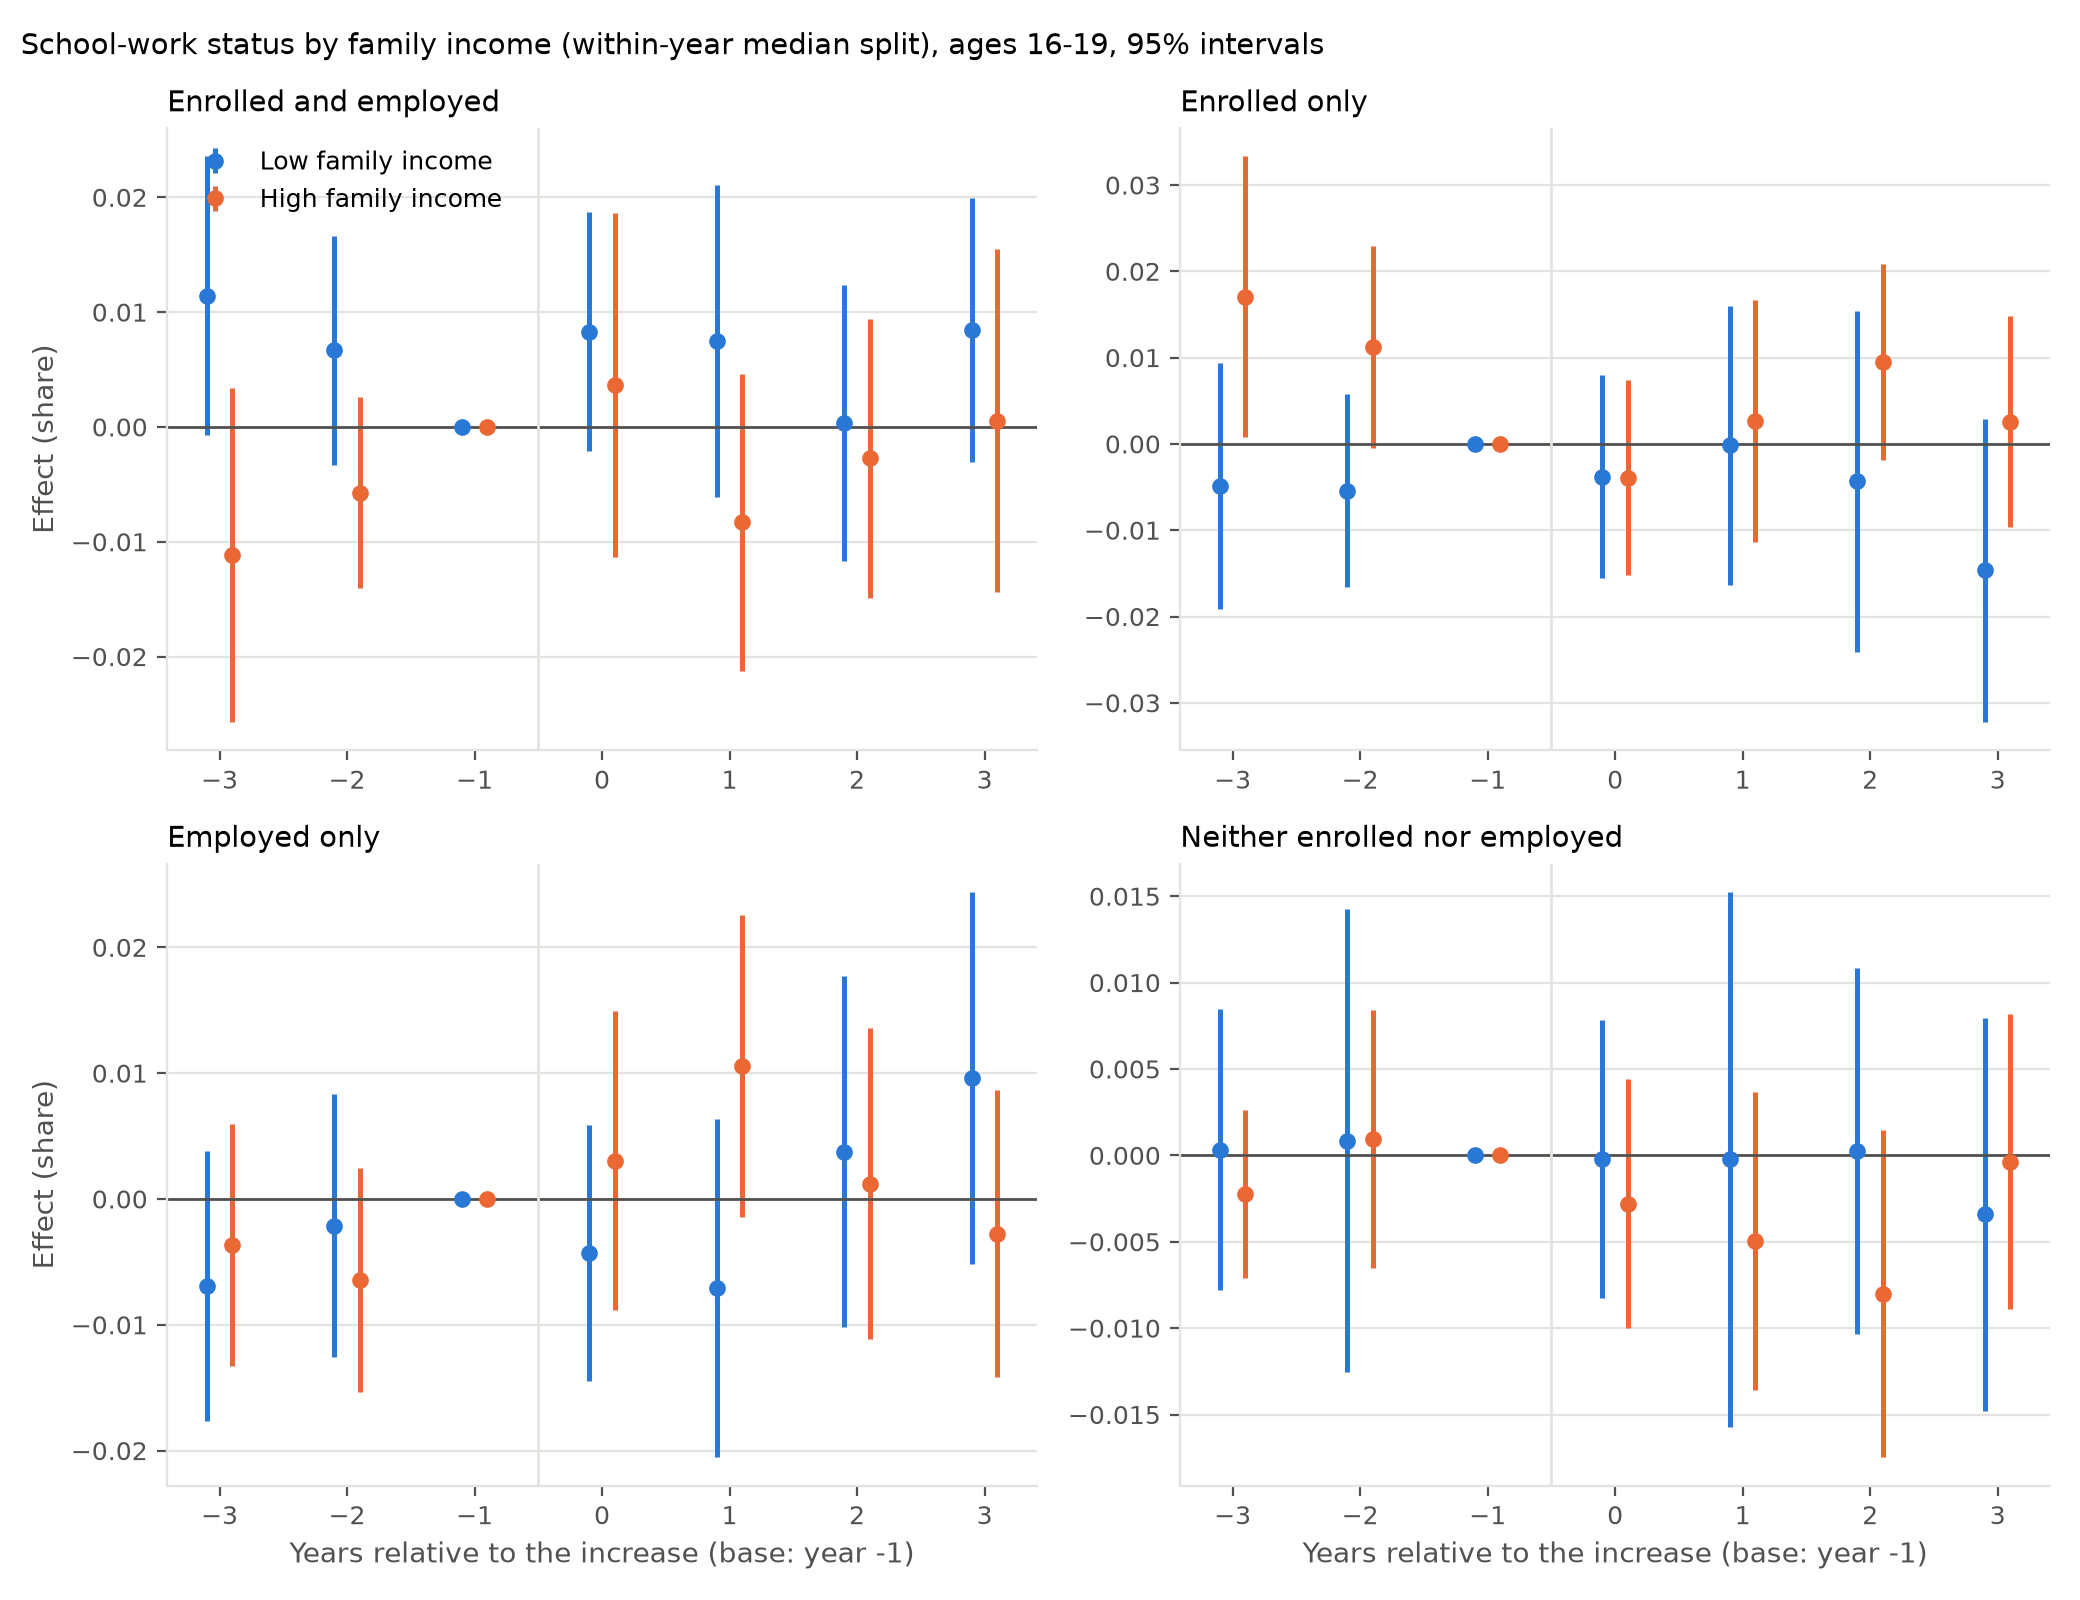
\includegraphics[width=\textwidth]{figures/figA_groups_sesrel.png}

\caption{Figure 14: Event-time effects on the four school--work shares by family income, within-year median split, ages 16--19}

\end{figure}


\section{E High school dropout}

Table 35 reports the effect on high school dropout, defined as in Smith (2021): not enrolled and without a diploma or GED. Because the basic monthly enrollment item records attendance last week, the measure is inflated in June, July and August (34 percent of 16--18 year olds against 6.4 percent in school months), so the table uses September to May, with the all-month estimate in the last column. Dropout does not fall. At ages 16--18, Smith's age range, the post-event average is $+0.5$ points (s.e.\ 0.4) on a base of 6.4 percent, with a pre-event average of $+0.3$; at 16--17 it is $+0.7$ (0.3) with a pre-event average of $+0.5$, and at 18--19 $+0.1$ (0.4). By family income the estimates are $+0.9$ (0.5) for low-income and $+0.6$ (0.4) for high-income 16--17 year olds, each with a pre-event average of about $+0.5$, and $-0.6$ (0.8) and $+0.2$ (0.4) at 18--19; the within-year median split gives the same. Net of the pre-event trend the post-event change is within a quarter of a point of zero in every cell. Smith's estimate, a 0.5 to 1.0 point fall in low-SES dropout per 10 percent rise in the minimum, implies a fall of 2 to 4 points for the increases studied here; the low-income intervals exclude a fall larger than about 0.5 points at 16--17 and 2 points at 18--19.

\begin{table}
\centering
\caption{Table 35: High school dropout (not enrolled, no diploma or GED): post-event averages, 73 events from 2010}

\small
\begin{tabular}{p{0.30\textwidth}p{0.113\textwidth}p{0.113\textwidth}p{0.113\textwidth}p{0.113\textwidth}p{0.113\textwidth}p{0.113\textwidth}}
\toprule
 & All & \multicolumn{2}{c}{Below / at or above \$50,000} & \multicolumn{2}{c}{Below / at or above median} & All months \\

 & Sept--May & Low & High & Low & High & \\
\midrule
Ages 16--17 & 0.007\textsuperscript{**} & 0.009\textsuperscript{*} & 0.006 & 0.008 & 0.006 & 0.004 \\
 & (0.003) & (0.005) & (0.004) & (0.005) & (0.004) & (0.005) \\
Ages 18--19 & 0.001 & -0.006 & 0.002 & -0.004 & 0.003 & -0.000 \\
 & (0.004) & (0.008) & (0.004) & (0.007) & (0.004) & (0.004) \\
Ages 16--18 & 0.004 & 0.005 & 0.005 & 0.004 & 0.005\textsuperscript{*} & 0.002 \\
 & (0.003) & (0.006) & (0.003) & (0.006) & (0.003) & (0.004) \\
Ages 16--19 & 0.004 & 0.002 & 0.004 & 0.003 & 0.005\textsuperscript{**} & 0.002 \\
 & (0.002) & (0.004) & (0.003) & (0.005) & (0.002) & (0.003) \\
\bottomrule
\end{tabular}



\noindent\small Notes: School months are September to May; the last column uses all months, in which summer non-attendance inflates the measure. Family income splits as in the main text and Appendix D. Block-bootstrap standard errors in parentheses.

\end{table}

\end{document}
